%!TEX root = ../template.tex
%%%%%%%%%%%%%%%%%%%%%%%%%%%%%%%%%%%%%%%%%%%%%%%%%%%%%%%%%%%%%%%%%%%%
%% chapter5.tex
%% NOVA thesis document file
%%
%% Chapter with lots of dummy text
%%%%%%%%%%%%%%%%%%%%%%%%%%%%%%%%%%%%%%%%%%%%%%%%%%%%%%%%%%%%%%%%%%%%

\typeout{NT FILE chapter5.tex}%

\chapter{Validation and Experimental Evaluation}\label{cha:validation}

In this chapter, we present the validation and experimental evaluation of the proposed solution. We start by discussing the evaluation criteria used to assess the quality of the present work, such as the used metrics to perform such measurements and the test benches employed. Then, we present the performance observations and results according to such criteria. 
Finally, we discuss the unobservability evaluation, and the formal validation of the proposed solution.

\section{Evaluation Criteria}\label{sec:evaluation_criteria}
To assess the quality of several aspects of the proposed solution, we defined a set of evaluation criteria as well as their importance to the overall system validation and evaluation. Tor is designed to protect users' privacy and anonymity, especially while web browsing, therefore is also important to evaluate the impact on performance. Tor already maintains a set of performance metrics and continuous evaluation, shared through Tor Metrics\footnote{\url{https://metrics.torproject.org/}}. Among several metrics and data collected by this project, we selected the most relevant and simple ones to compare our solution. Regarding performance, we used the standardized activity to evaluate the performance: \textit{download a file}. Tor Metrics uses 3 different file sizes to evaluate Tor: 50 KiB, 1 MiB and 5 MiB. Given this, we also tested our solution by downloading files of these sizes and compared the results regarding the throughput, the total time to download such files and the circuit round-trip latencies of circuits. 

Also, given the solution's goal to enhance Tor users' privacy and anonymity guarantees, we also considered the impact on the unobservability of the traffic. To evaluate the resistance of the solution, especially against attacks targeting website fingerprinting, such as the ones pointed out throughout this work as those carried by our adversaries, we conducted fingerprinting resistance tests. This tests allowed for a better understanding of the impact of the proposed solution on the unobservability of the traffic, and therefore on the anonymity guarantees. 

Finally, to demonstrate Differential Privacy benefits, we also performed a formal validation of the proposed solution, to express the privacy guarantees provided by the solution, using mathematical formalism and Different Privacy theorems.

\subsection{Test Benches}\label{sec:testbenches}

To conduct the before-mentioned tests, we design a couple of test benches to enlarge the scope of validation and evaluation of the solution. The testing environment for all test benches was design to be as close as possible to a real world scenario and to grant easy replication and deployability of such tests and results, by deploying two types of Tor networks:
\paragraph{Local Simulated Network} This tests bench focused on validating the solutions' extension of Tor, by simulating a minimal Tor network, with 4 relays (directory authority, 2 non-exit relays and 1 exit relay) and Tor client on a Docker Composed system on a single machine. Even though this scenario does not replicate the exact conditions of a real Tor network, this was an important stage to learn and test how to create and deploy a private minimal Tor network, as well as to test and validate the solution's intended behavior. This test bench was performed on a single 2 vCores OVH\footnote{\url{https://www.ovhcloud.com/pt/}} Virtual Private Server (VPS) with 4 GB of RAM, configured with Ubuntu 24.10.
\paragraph{Distributed Network} This test bench aimed to evaluate our solution in a more realistic scenario, by emulating a small private distributed Tor network, with 4 relays and a Tor client, each deployed on a separate OVH VPS using Docker Swarm. On the tests. This test bench allowed us to evaluate the performance and unobservability of our solution in a more realistic environment, with network latencies and conditions closer to those of the real Tor network. This test bench was performed using 5 OVH VPSs, each with 2 vCores and 4 GB of RAM, configured with Ubuntu 24.10. These machines were dispersed through France, Germany, Poland and the United Kingdom.

\subsection{Experimental Observations}\label{sec:experimental_observations}

Our solution produced results for both performance and unobservability evaluations. The performance observations were performed using the \texttt{curl} command to download files of different sizes. The files were generated by a simple \textit{Python} web server hosted by our private network as a container, present in the directory authority machine, in case of the distributed test bench. The used command was:

\begin{lstlisting}[language=bash]
  $  curl --socks5 <tor_proxy> -H 'Cache-Control: no-cache' \
        -w 'Code: %{response_code}\n
           Time to first byte: %{time_starttransfer}s\n
           Total time: %{time_total}s\n
           Download speed: %{speed_download} bytes/sec\n' \
        -o /dev/null \
        <file_server_ip>:<file_server_port>/bytes/<file_size_in_bytes>
\end{lstlisting}

The \texttt{`socks5'} flag is required to route the traffic through the Tor network, therefore the \texttt{<tor\_proxy>} must be a tor client node. As mentioned before in~\autoref{subsec:deployment_for_validation_and_testing}, we recommend this request to be performed in the client node's machine and to assing the value \textit{`127.0.0.1:9000'} to \texttt{<tor\_proxy>}. The \texttt{file\_server\_ip} and \texttt{file\_server\_port} refer to the web server and, as the name suggests, the \texttt{file\_size\_in\_bytes} refers to the size of the file to be downloaded, in bytes. The used sizes were $51200$ bytes, $1 048 576$ bytes 5 242 880 bytes, respectively the files used by Tor Metrics. The \texttt{-H 'Cache-Control: no-cache'} flag is used to prevent caching of the file, ensuring that each download request retrieves the file from the server rather than a cached version. The \texttt{-w} flag is used to format the output of the command, displaying the HTTP response code, for debugging purposes, time to first byte, to capture the latency, total time taken for the download, and download speed in bytes per second, referred onwards as throughput.

To collect data for the unobservability evaluation, we used the previous work of~\citeauthor{MIRACE}\cite{MIRACE}, by capturing traffic using \texttt{tcpdump} to \textit{pcap} files and then using the captured traces to trains and evaluate machine learning models to simulate website fingerprinting attacks. 

\section{Performance Evaluation}\label{sec:performance_evaluation}

To evaluate the performance of our solution, we conducted a series of experiments to measure the impact of the implemented features alone and in combination. In this section, we present the performance evaluation results, focusing on each metric. Firstly, we address the throughput results, followed by the total time taken to download files of different sizes, and finally, we analyze the latency results and the effect of the PPC feature on false cells and TLS packets count. 

The experiments were performed with variable configurations for both features. The Packet Padding Cells feature was tested with different $\epsilon$ values, ranging from 0 to 5, with more collections between 0 and 1, variable onwards referred as $\epsilon_d$. On the other hand, the Schedulers feature was also tested with different $\epsilon$ values, also ranging from 0 to 5, with more collections between 0 and 1, variable onwards referred as $\epsilon_j$. Additionally, when individually testing the Schedulers, we used different mathematical distributions to generate jitter: \textit{Poisson} and \textit{Exponential}. We also tested both features together, with variable $\epsilon_d$ and $\epsilon_j$ values, using the \textit{Poisson} distribution for jitter generation, due to time limitations of this work. These results are represented by heatmaps, with each $\epsilon$ as an axis, as the heat as the value of the metric.

In addition, we also present some results regarding the number of Packet Padding Cells generated during the experiments, compared with the TLS packets and total cells.

As mentioned earlier, the Tor Metrics project provides a continuous evaluation of the Tor network, including performance metrics such as throughput, total time to download files, and latency. In this chapter, we present our results and compare to the most recent results on Tor Metrics. The project provides results for 6 types of sources, but we focus on those which do not include the Conflux network, represented as mean of all medians. Conflux is a traffic splitting feature that Tor leverages to improve performance but, considering that our tests were conducted in a controlled and minimal network of relay, this features had no effect and must not be considered for results comparison. 

All experiments were conducted in the environments described in~\autoref{sec:evaluation_criteria} and compared with control tests performed without the implemented features, for baseline performance measurement, and with the Tor Metrics measures at the time of writing. The values presented in the following sections were obtained by performing a download 100 times for each configuration and calculating the median, 10th and 90th percentiles.

\subsection{Throughput}
Throughput is the unit of measurement that represents the amount of data flowing throw a certain point in the network. In our case, the throughput of the network is retrieved by downloading a file and measuring the download speed, in bytes per second. This is an important metric to evaluate the performance of our solution, as it directly impacts the user experience when browsing the web.

Below we share the throughput results obtained from our experiments and according to the above-mentioned test benches. We present the results for the local simulated environment in~\autoref{fig:local_throughput} and the distributed environment in~\autoref{fig:dist_throughput}. Each contains the corresponding results for each feature alone and both features combined, with the median represented as a thick line, together with a shaded area representing the first and third quartiles.

\begin{figure}[htbp]
    \centering
    \begin{subcaptionbox}{Only Packet Padding Cells Feature}[0.45\textwidth]
        {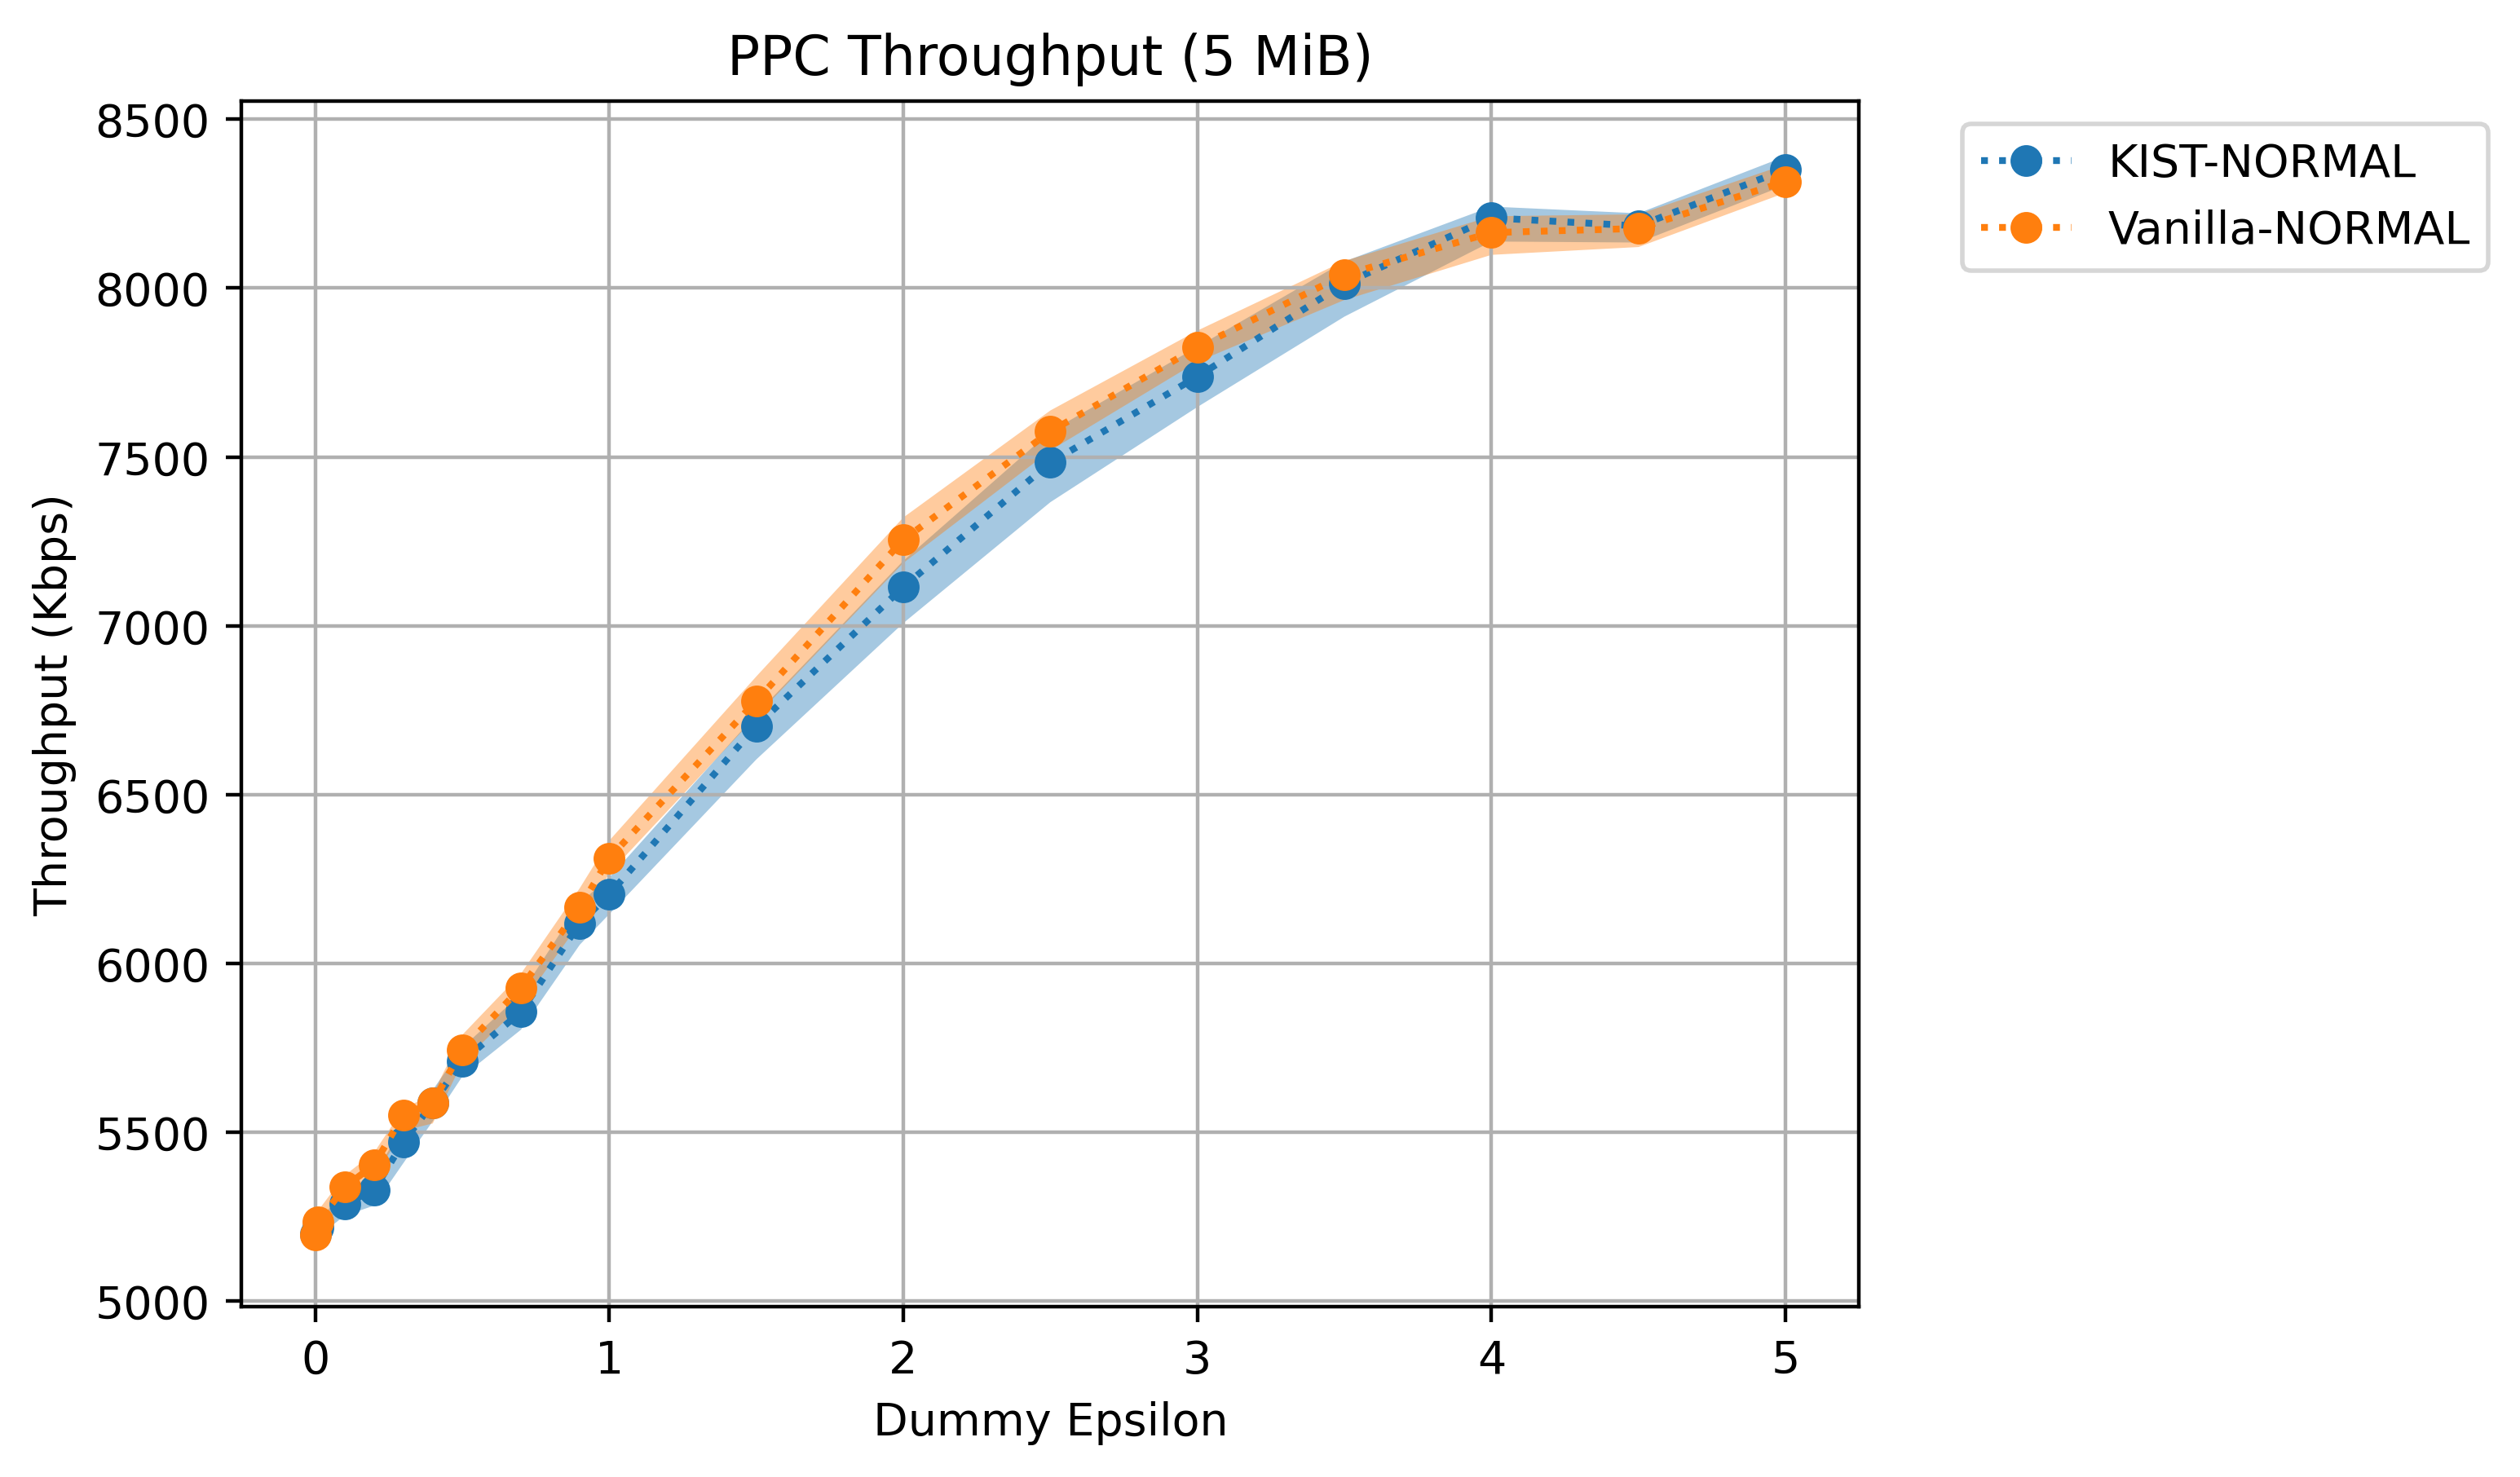
\includegraphics[width=\linewidth]{Chapters/Figures/Plots/local_throughput_50_PPC_5mib.png}\label{fig:local_ppc_throughput}}
    \end{subcaptionbox}
    \hfill
    \begin{subcaptionbox}{Only Jitter Injection Schedulers Feature\label{fig:local_jitter_throughput}}[0.45\textwidth]
        {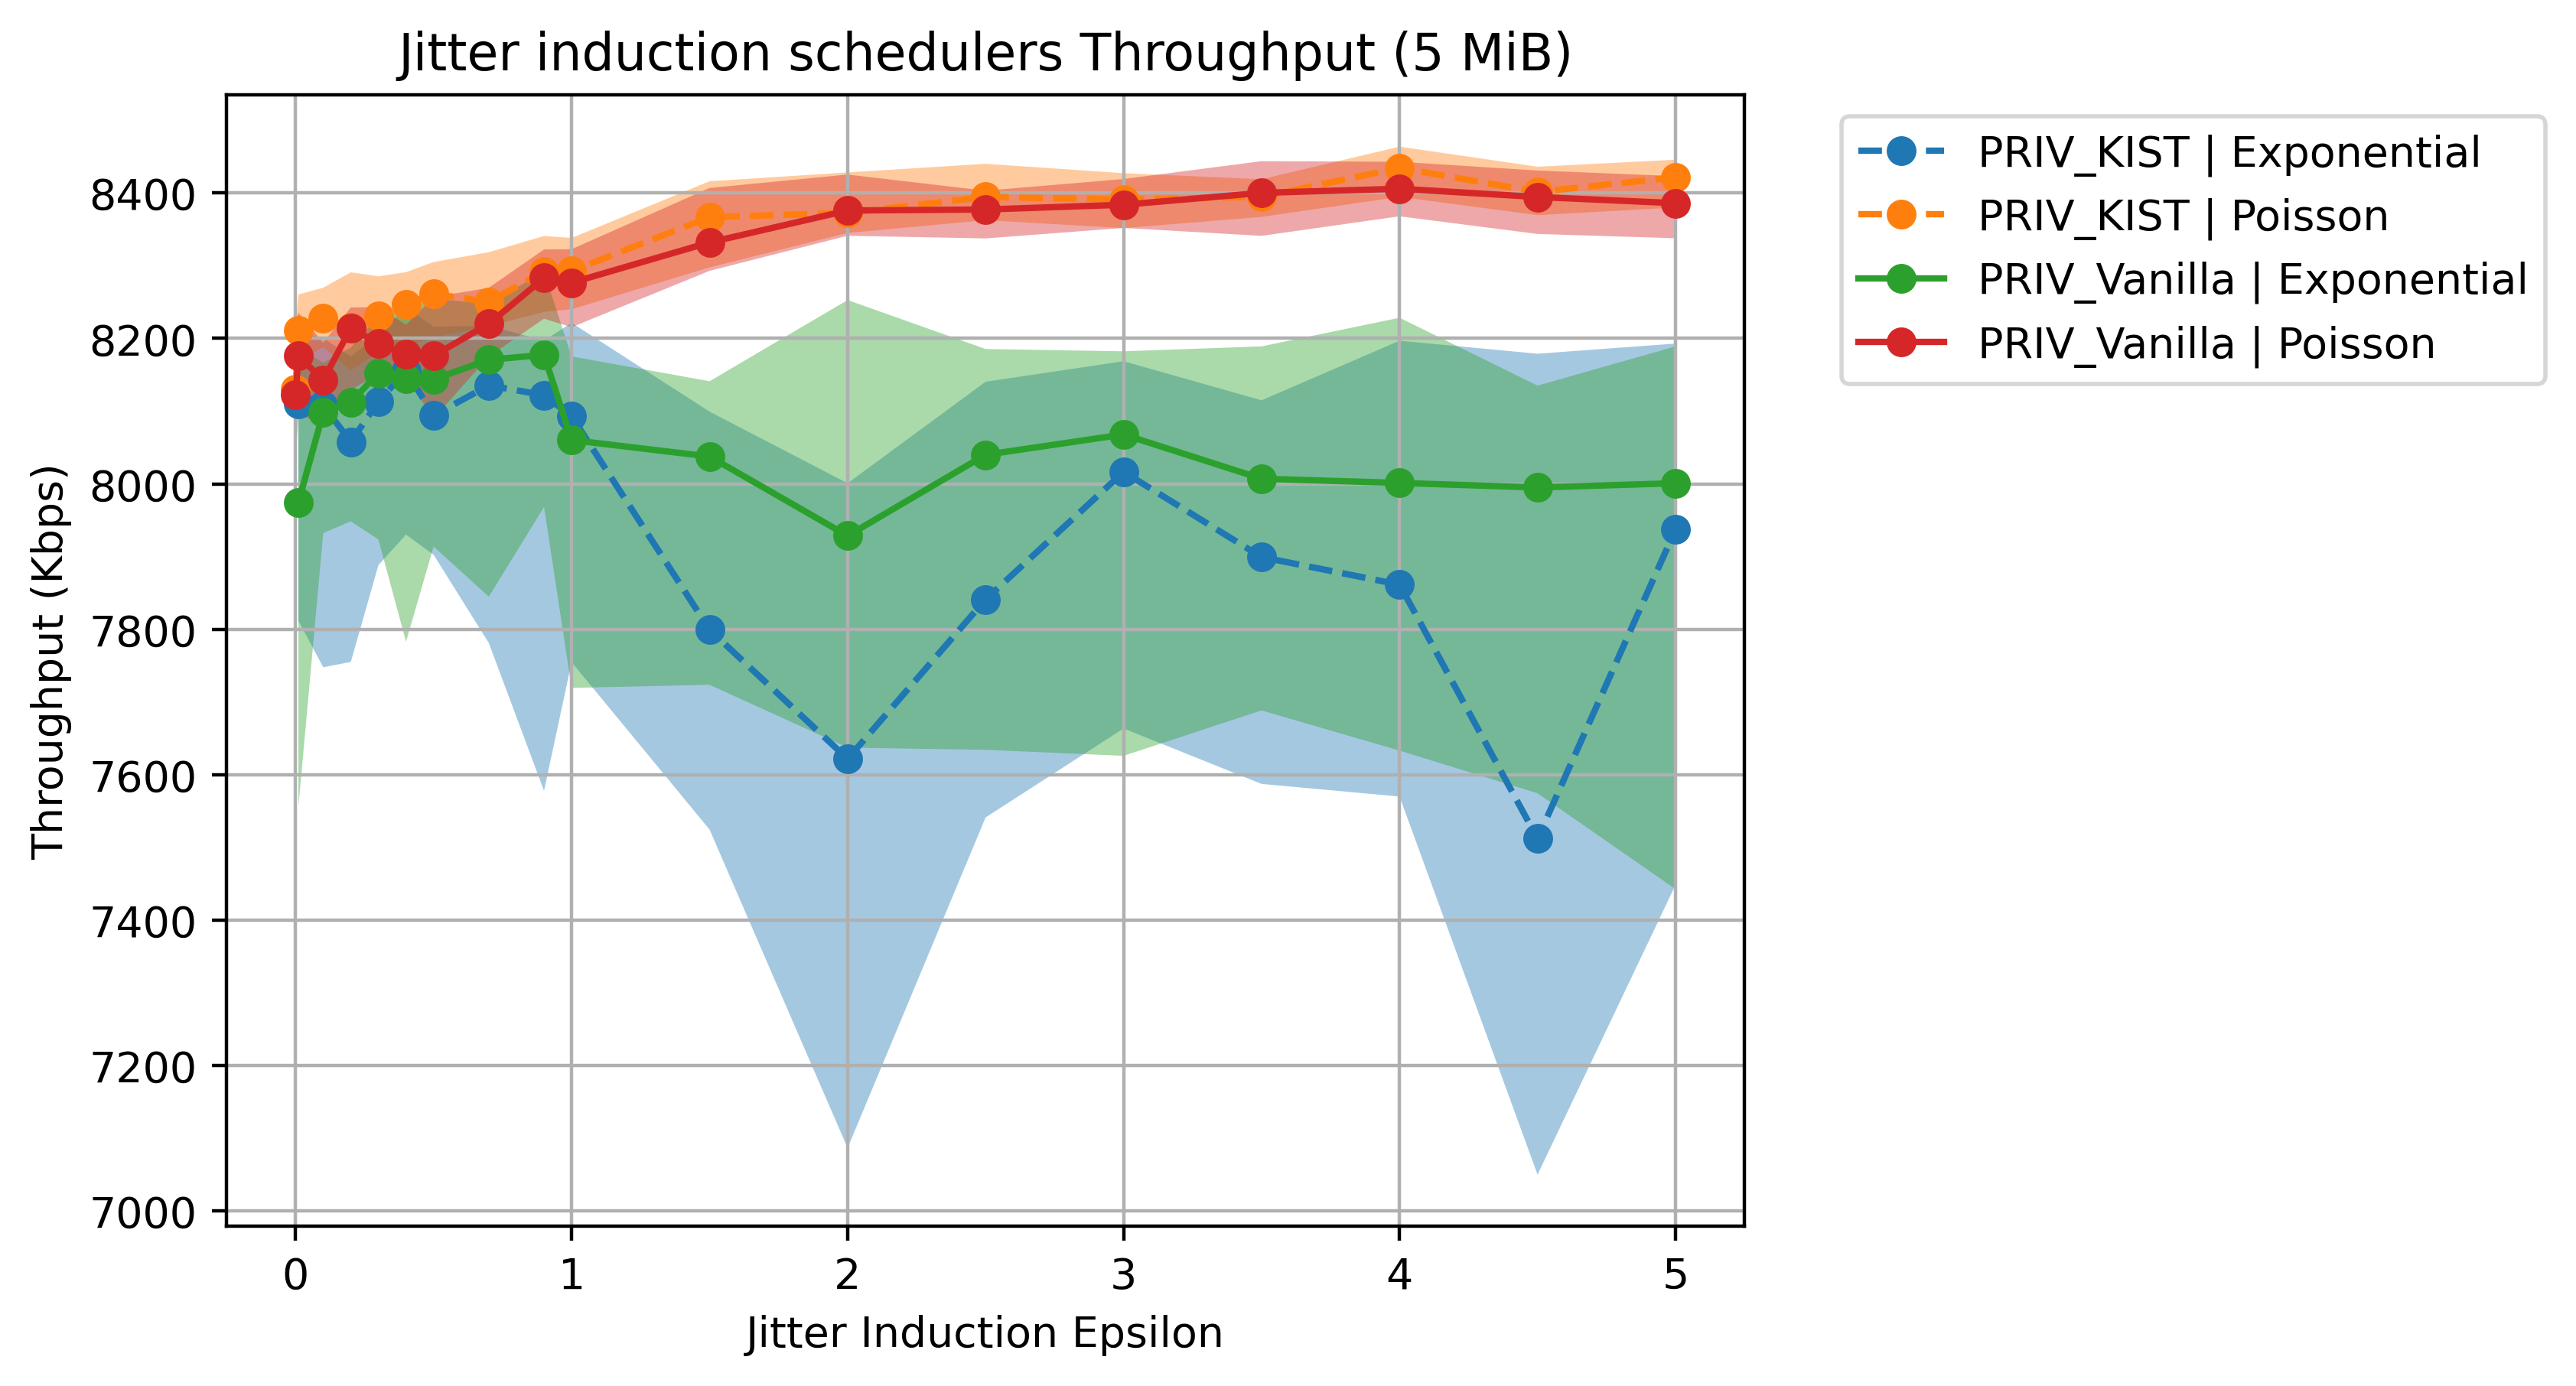
\includegraphics[width=\linewidth]{Chapters/Figures/Plots/local_throughput_50_jitter_5mib.png}}
    \end{subcaptionbox}
    \vfill
    \begin{subcaptionbox}{Both Features\label{fig:local_both_throughput}}[0.65\textwidth]
        {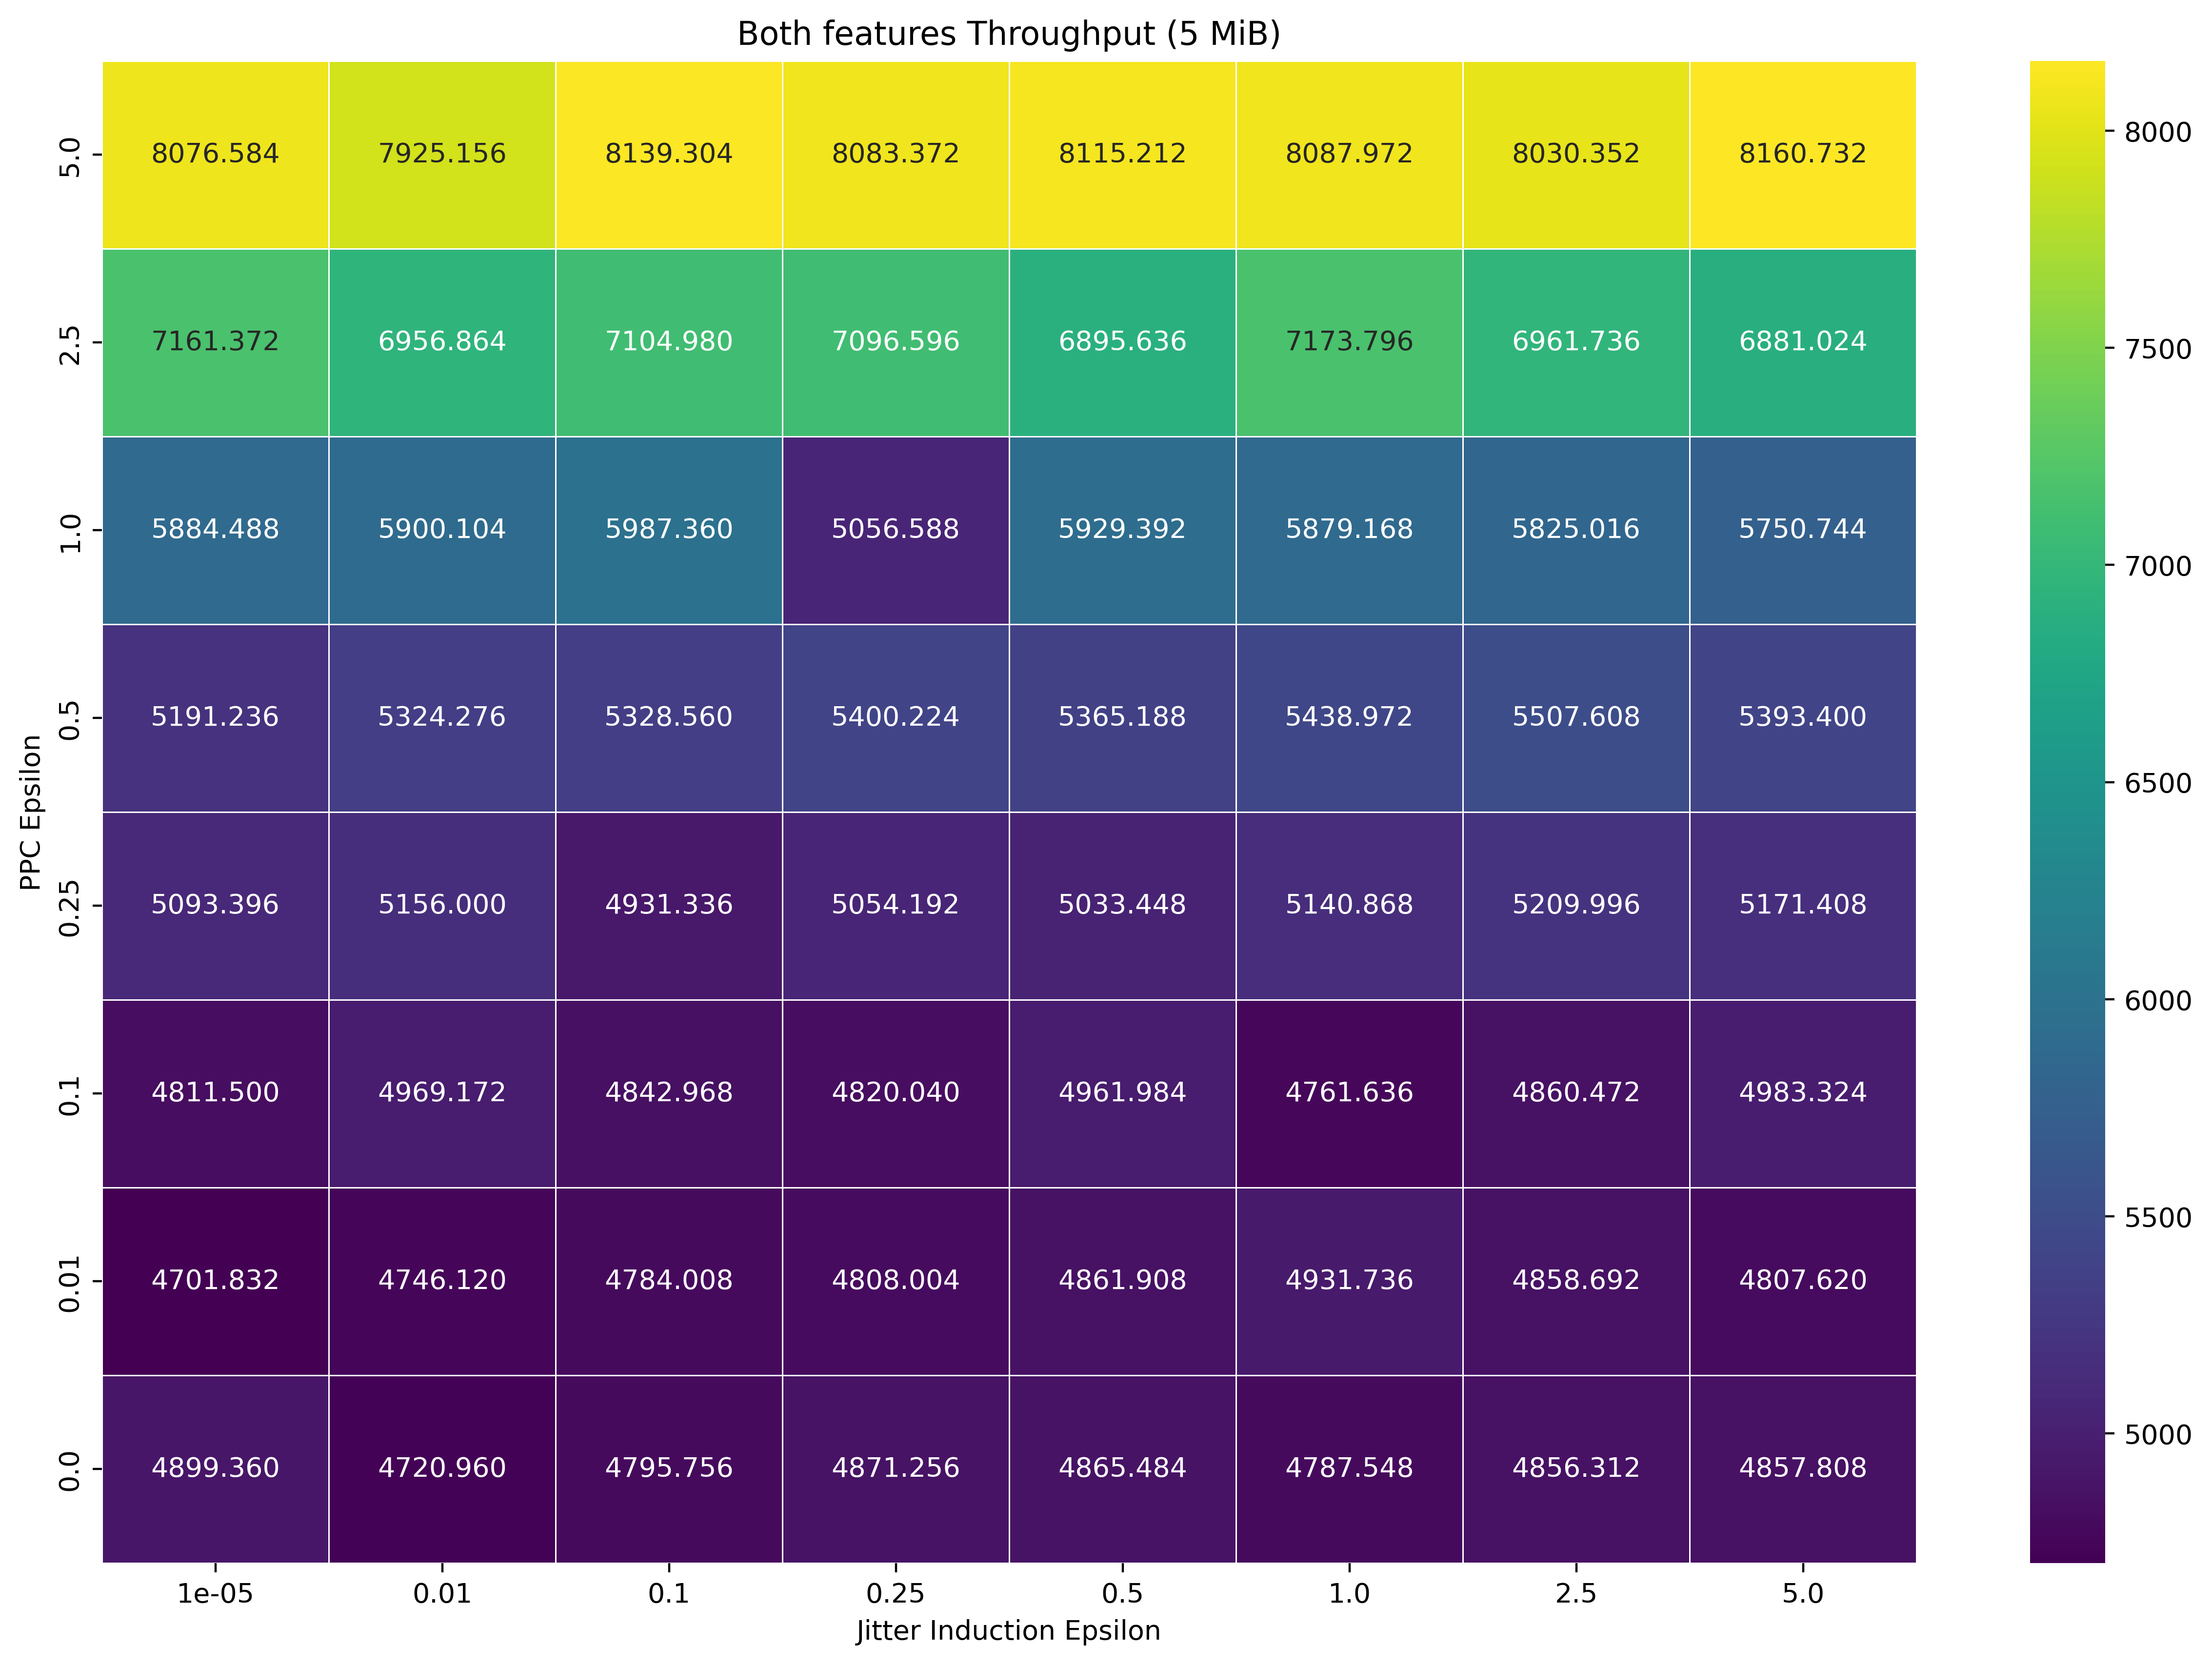
\includegraphics[width=\linewidth]{Chapters/Figures/Plots/local_throughput_50_heatmap_5mib.png}}
    \end{subcaptionbox}
    \caption{Throughput Results on Local Simulated Environment}\label{fig:local_throughput}
\end{figure}

\begin{figure}[htbp]
    \centering
    \caption{Throughput Results on Distributed Environment}\label{fig:dist_throughput}
    \begin{subcaptionbox}{Only Packet Padding Cells Feature\label{fig:dist_ppc_throughput}}[0.45\textwidth]
        {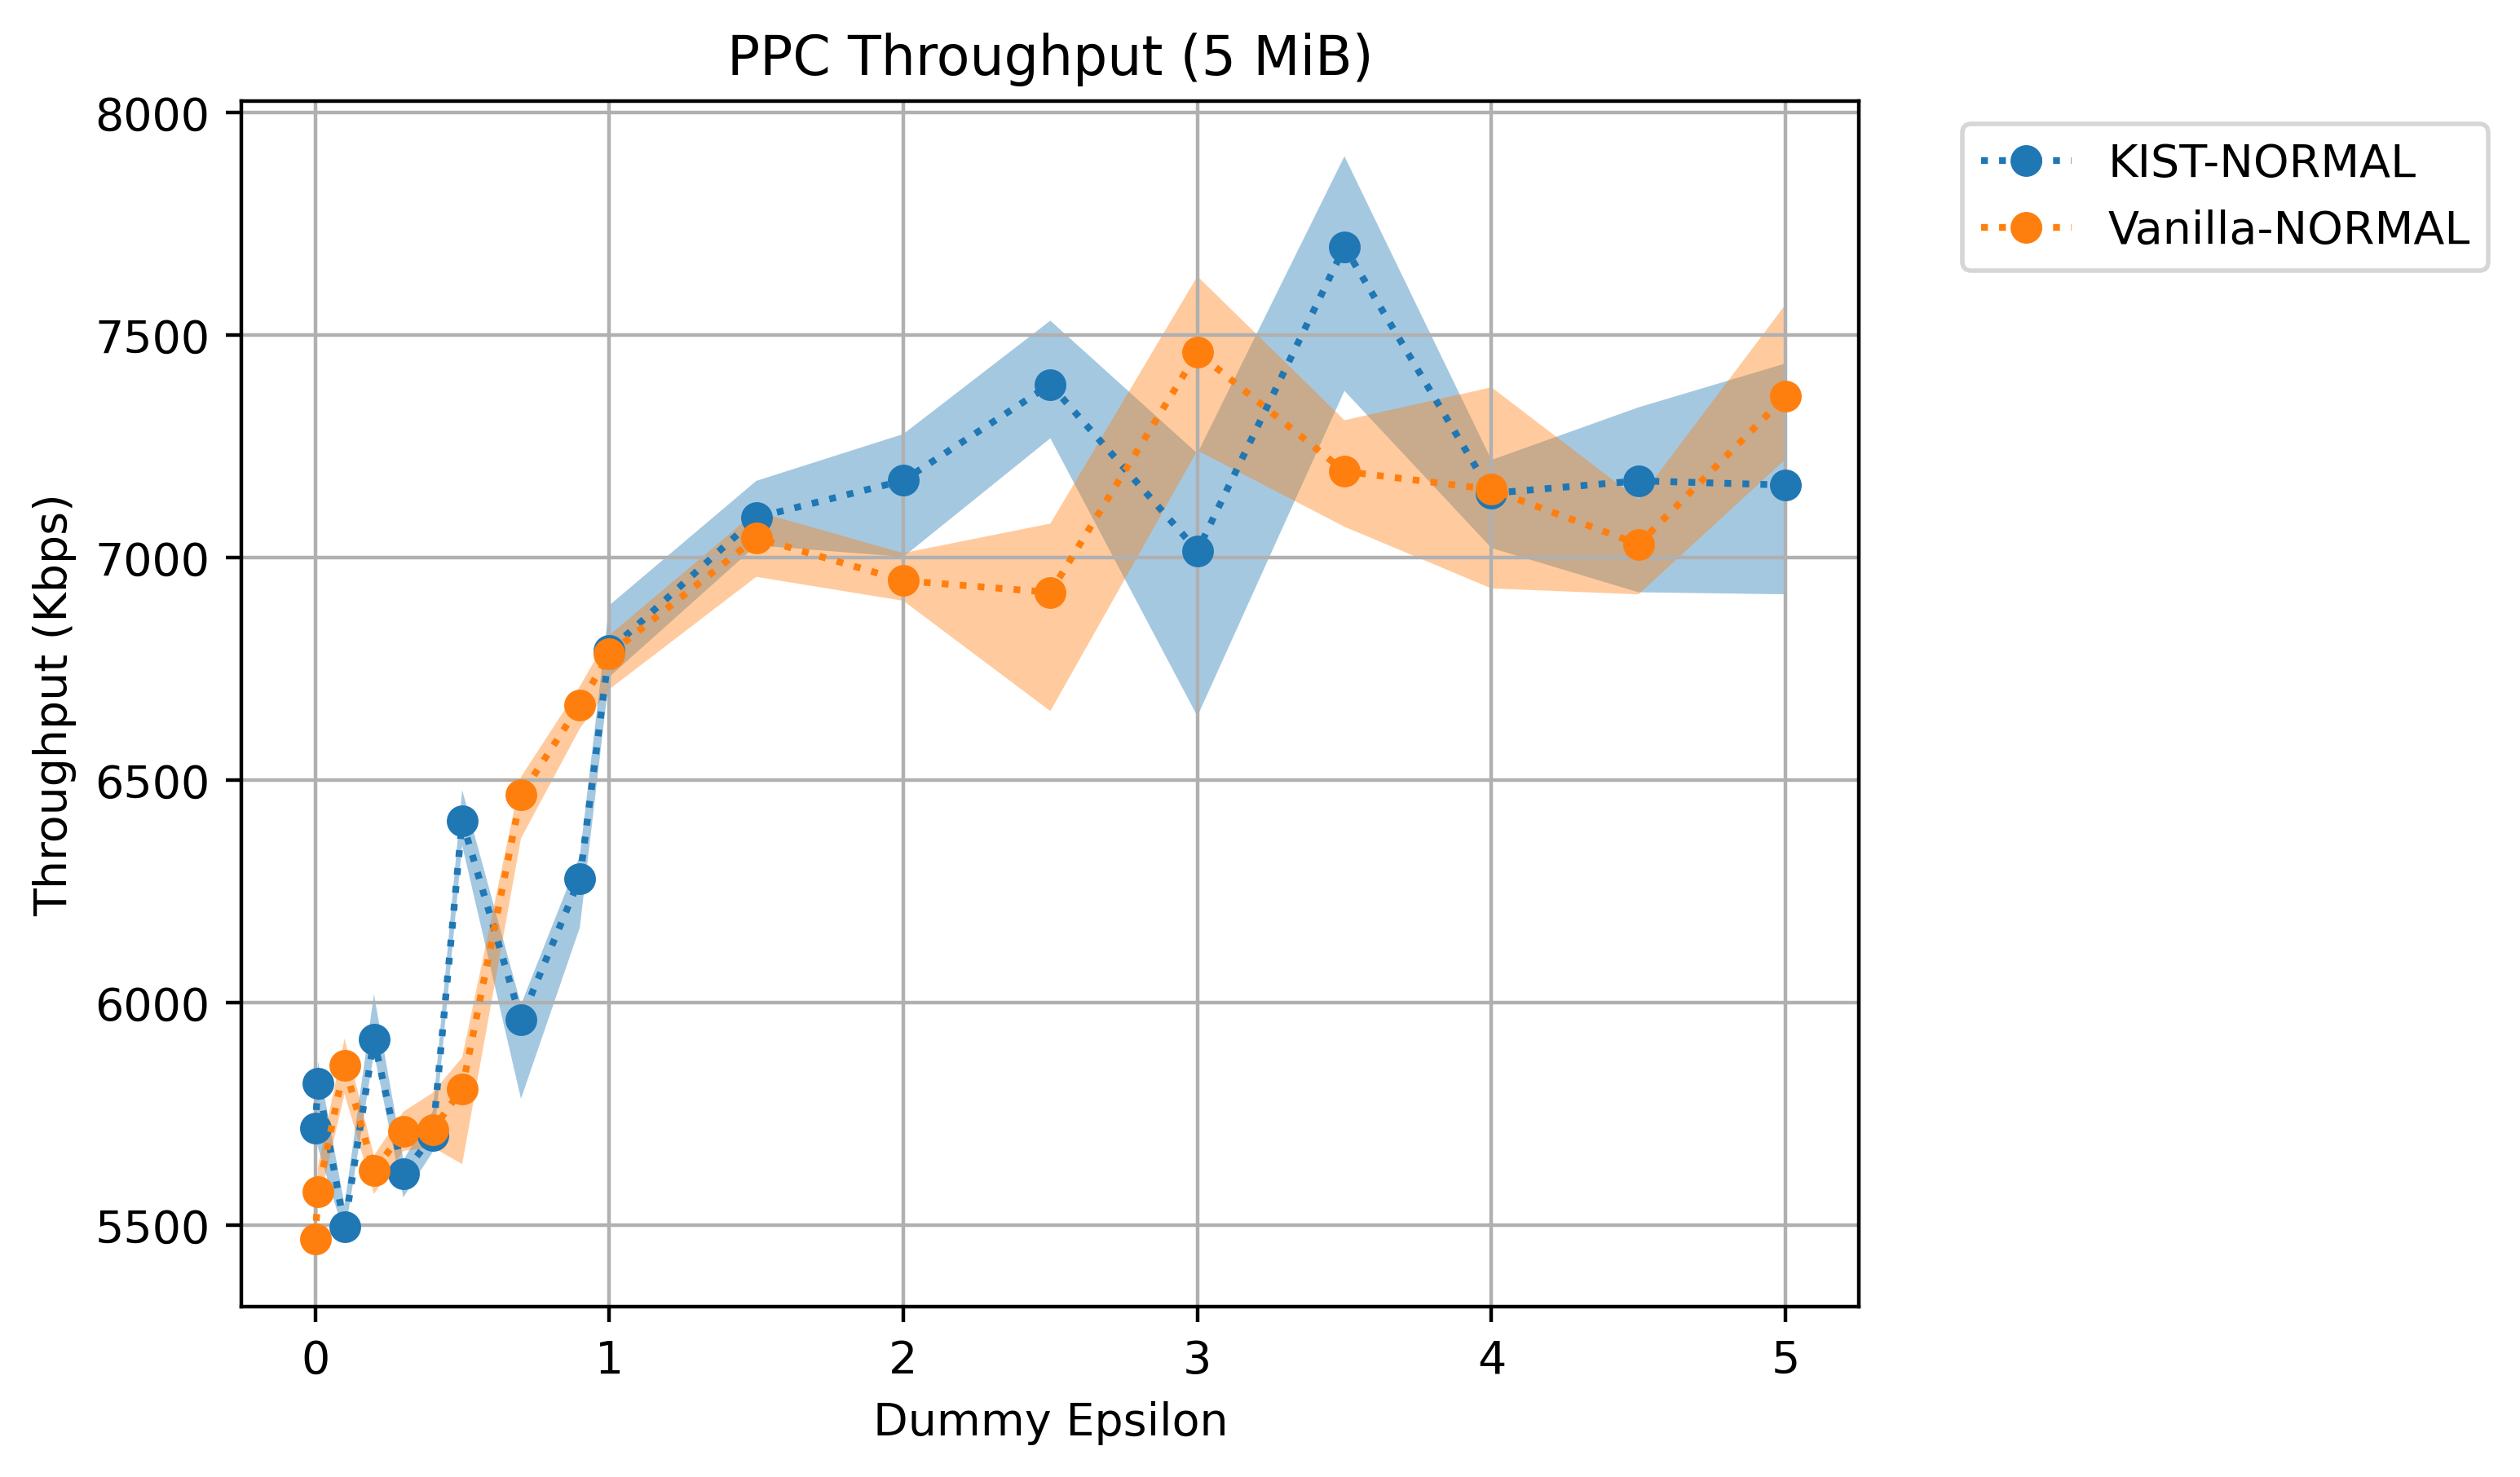
\includegraphics[width=\linewidth]{Chapters/Figures/Plots/dist_throughput_50_PPC_5mib.png}}
    \end{subcaptionbox}
    \hfill
    \begin{subcaptionbox}{Only Jitter Injection Schedulers Feature\label{fig:dist_jitter_throughput}}[0.45\textwidth]
        {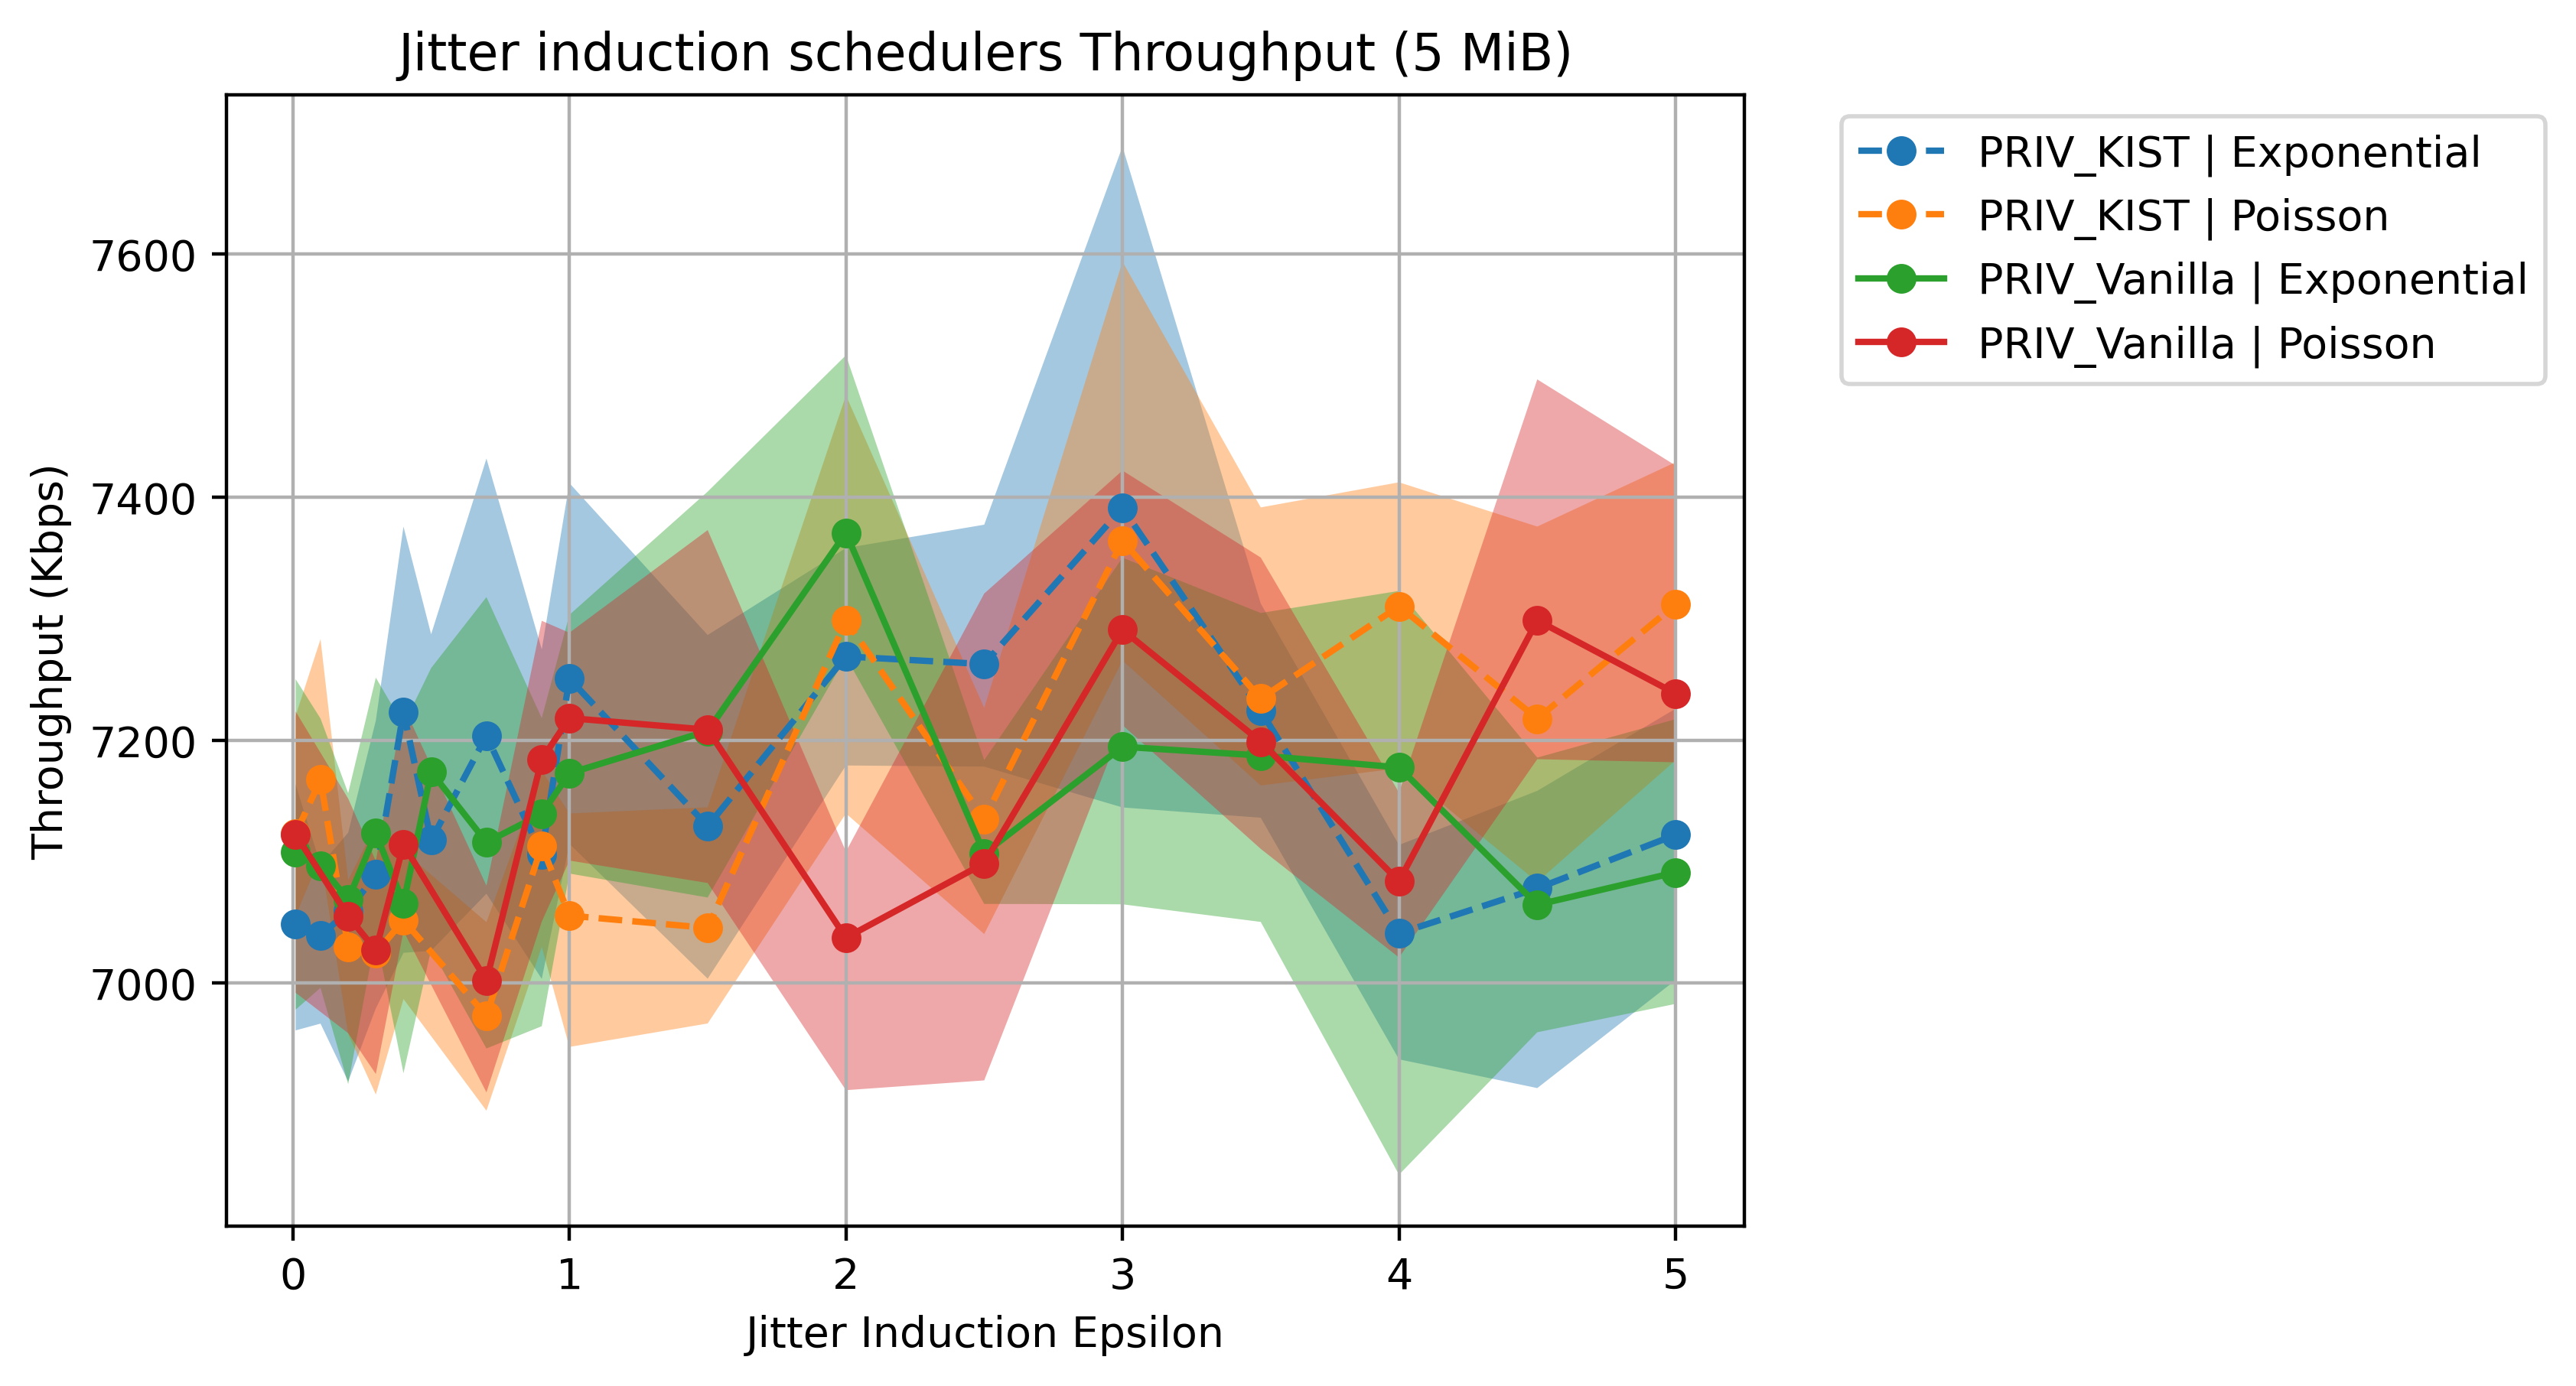
\includegraphics[width=\linewidth]{Chapters/Figures/Plots/dist_throughput_50_jitter_5mib.png}}
    \end{subcaptionbox}
    \vfill
    \begin{subcaptionbox}{Both Features\label{fig:dist_both_throughput}}[0.65\textwidth]
        {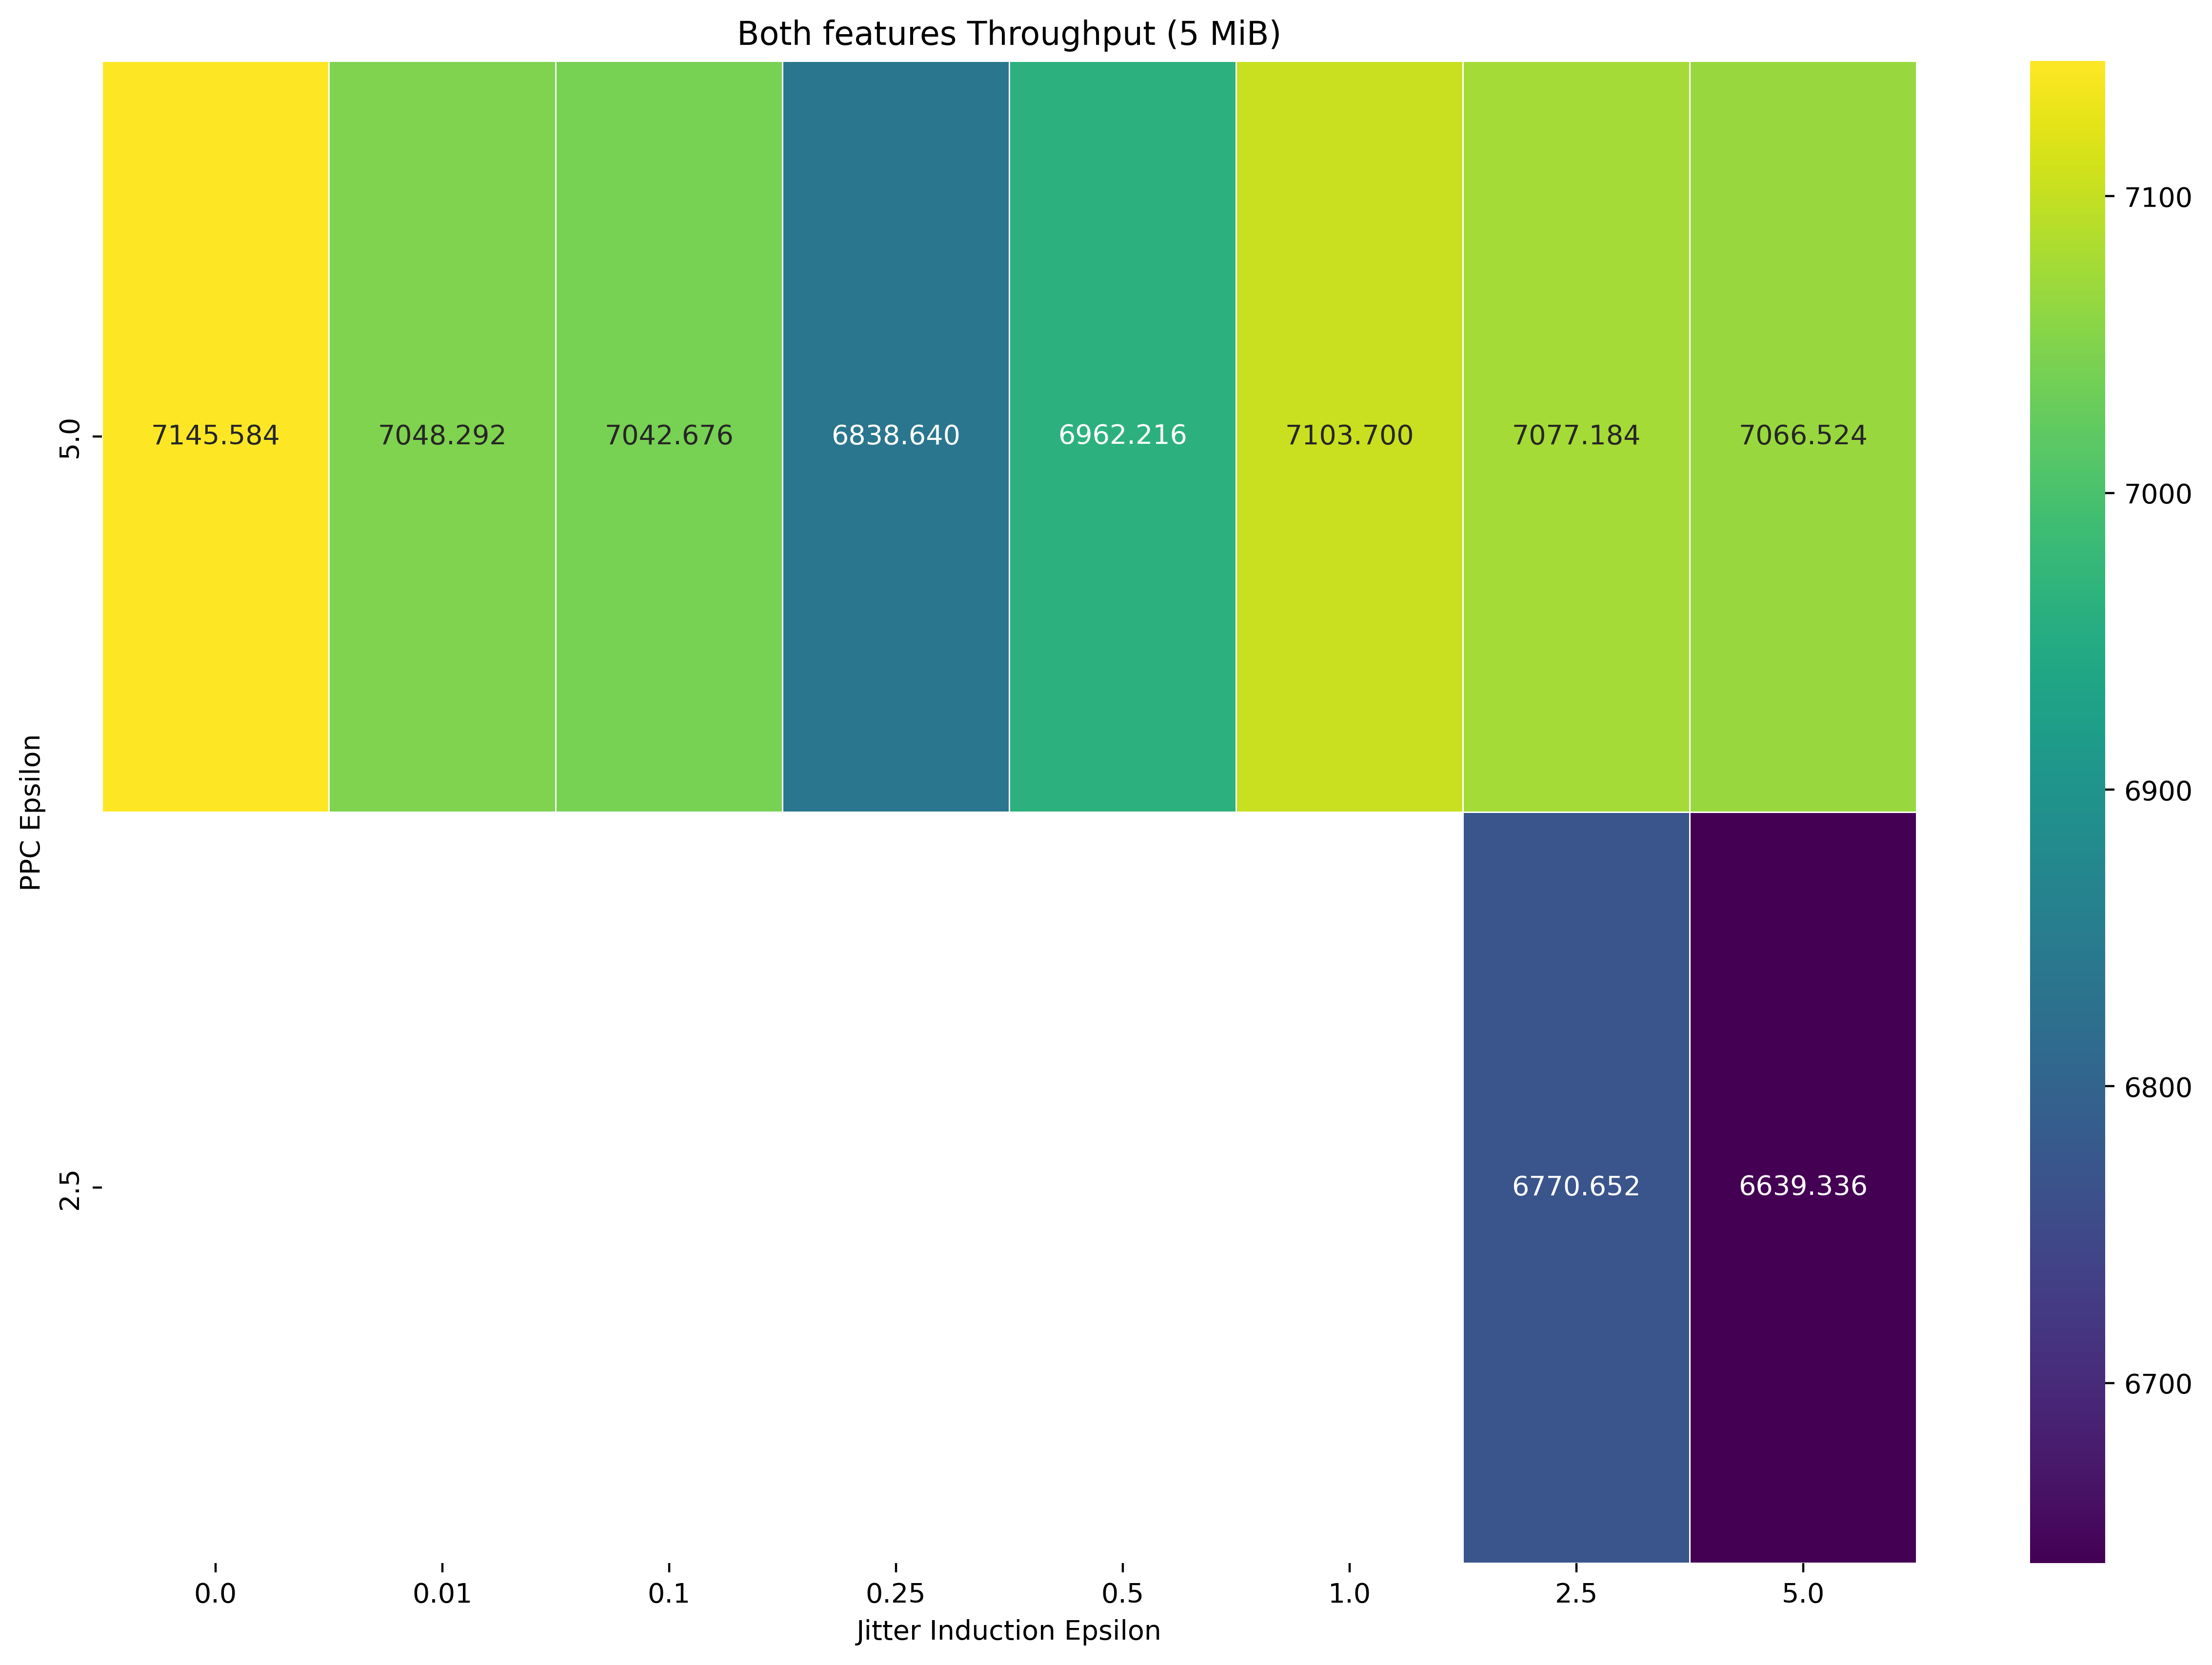
\includegraphics[width=\linewidth]{Chapters/Figures/Plots/dist_throughput_50_heatmap_5mib.png}}
    \end{subcaptionbox}
\end{figure}

As shown in~\autoref{fig:local_throughput} and~\autoref{fig:dist_throughput}, the PPC feature has a more significant impact on throughput than the Schedulers feature. 
This impact has greater impact as $\epsilon_{PPC}$ decrease, reaches a plateau when $\epsilon_{PPC}$ is greater than 4. The distributed test bench showed more unstable results, but the overall trend is similar. The Schedulers feature has a smaller impact on throughput, with a slight decrease for $\epsilon_{J}$ values closer to 0. Unexpectably, in the Local Emulated test bench, the Exponential distribution increases its variance on tests with $\epsilon_{J}$ greater than 1, but the throughput get slightly worse. 
In all experiments, all types schedulers behaved similarly.
For the experiments with both features enabled, the results emphasized the greater impact of the PPC feature on throughput. The heatmap clearly shows that the throughput only oscillate vertically, but remain consistent across different $\epsilon_{J}$ values.

As time of writing, Tor Metrics reports a median throughput value of 18 236 Mbps for files downloaded over the Tor network. Although, is important to note that these values are sampled from downloads of different files and only measure the throughput value between 4 MiB and 5 MiB of such files. In our case, we compare this value with the throughput values obtained from downloading files of 5 MiB.
%TODO: MUST TEST COMBINATIONS ON DISTRIBUTED TO GET BETTER ANALYSIS ON WORSE/BETTER TEST BENCH AND CONFIGURATION

\begin{table}[htbp]
    \centering
    \begin{tabular}{|c|c|c|}
    \hline
    \textbf{Configuration} & \textbf{Local} & \textbf{Distributed} \\
    \hline
    Tor Metrics& \multicolumn{2}{c|}{11 587} \\ 
    \hline
    \multirow{2}{*}{Control} & 8 240 & 7 045\\ 
    & 8 235 & 7 298\\
    \hline
    Only PPC & 5 197 – 8 351 & 5 469 – 7 699\\
    \hline
    Only Jitter & 7 512 – 8 435 & 6 973 – 7 391\\
    \hline
    PPC \& Jitter & 4 721 – 8 161 & 6 639 – 7 146\\
    \hline
    \end{tabular}
    \caption{Throughput Results Summary (Mbps)}\label{tab:throughput_summary}
\end{table}

\FloatBarrier
\subsection{Total Time}

Evaluating the total time necessary to download a file is also important to understand the effects of our solution on user experience and performance. Therefore, we present the total time results obtained from our experiments in~\autoref{fig:local_total_time} for the local simulated environment and~\autoref{fig:dist_total_time} for the distributed environment. We followed the Tor Metrics directives and also present the results as a thick line which represents the median value, together with a shaded area representing the first and third quartiles.

\begin{figure}[htbp]
    \centering
    \begin{subcaptionbox}{Only Packet Padding Cells Feature\label{fig:local_ppc_total_time}}[0.45\textwidth]
        {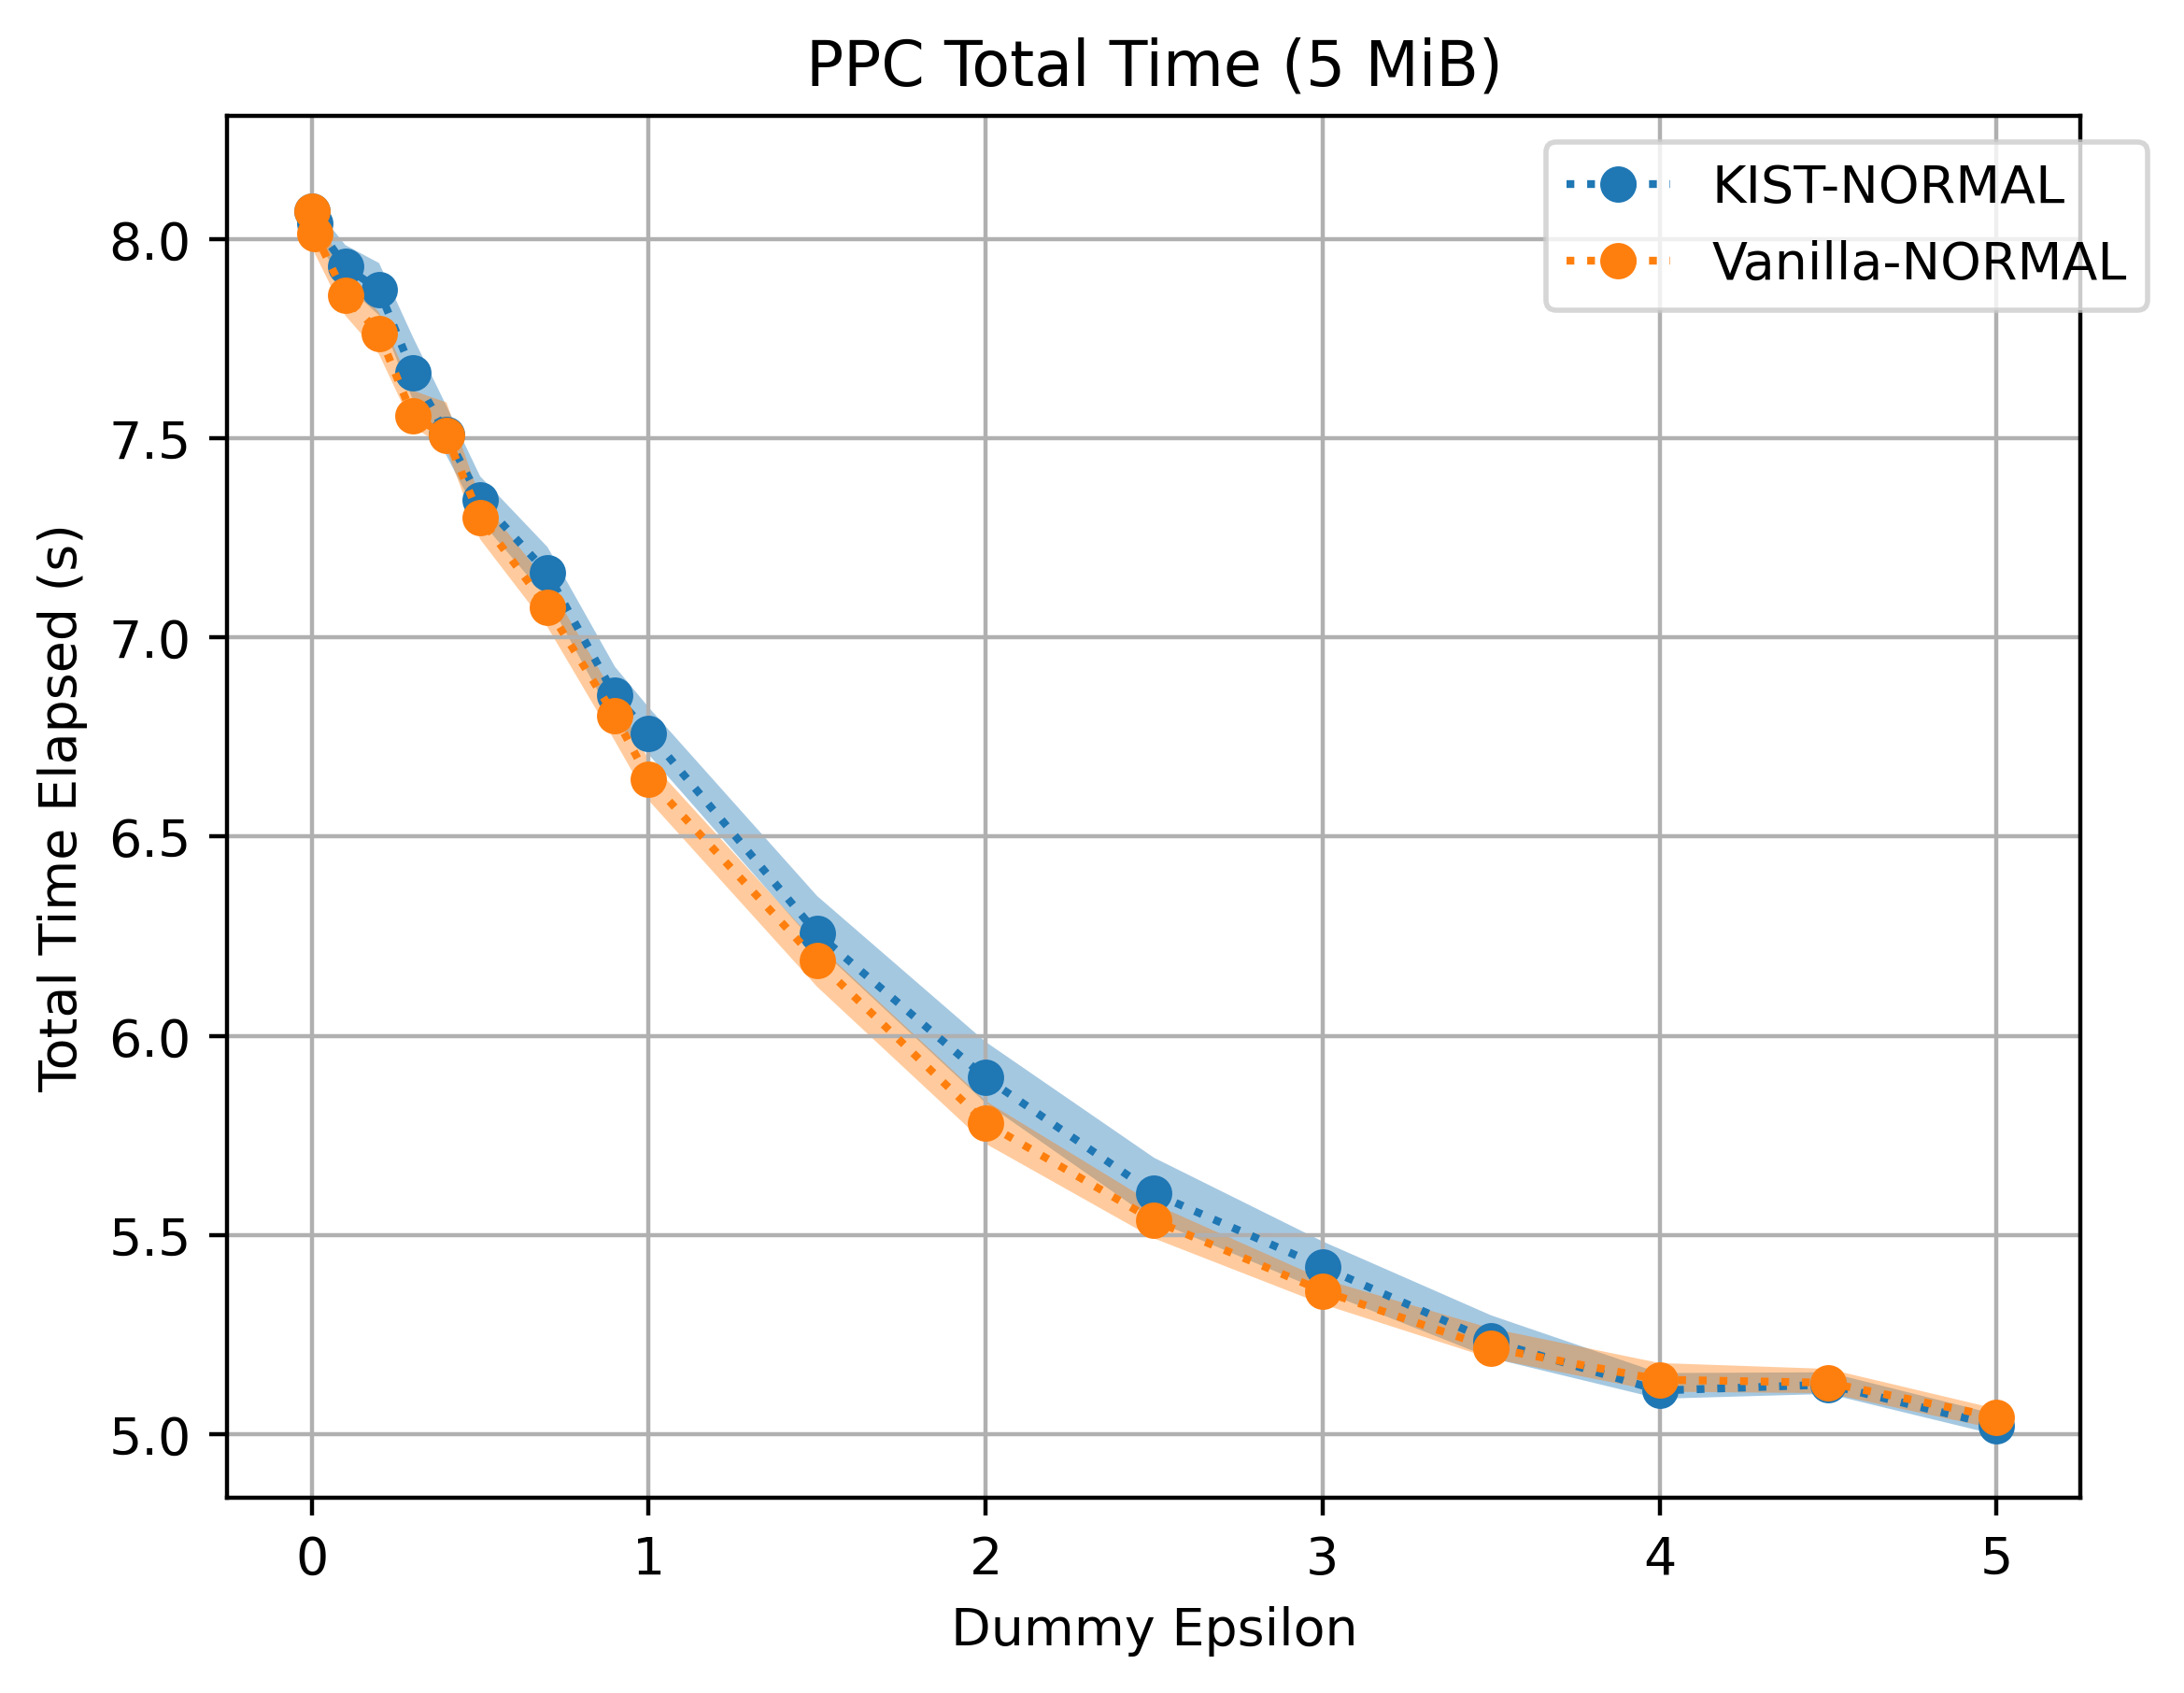
\includegraphics[width=\linewidth]{Chapters/Figures/Plots/local_total_time_50_PPC_5mib.png}}
    \end{subcaptionbox}
    \hfill
    \begin{subcaptionbox}{Only Jitter Injection Schedulers Feature\label{fig:local_jitter_total_time}}[0.45\textwidth]
        {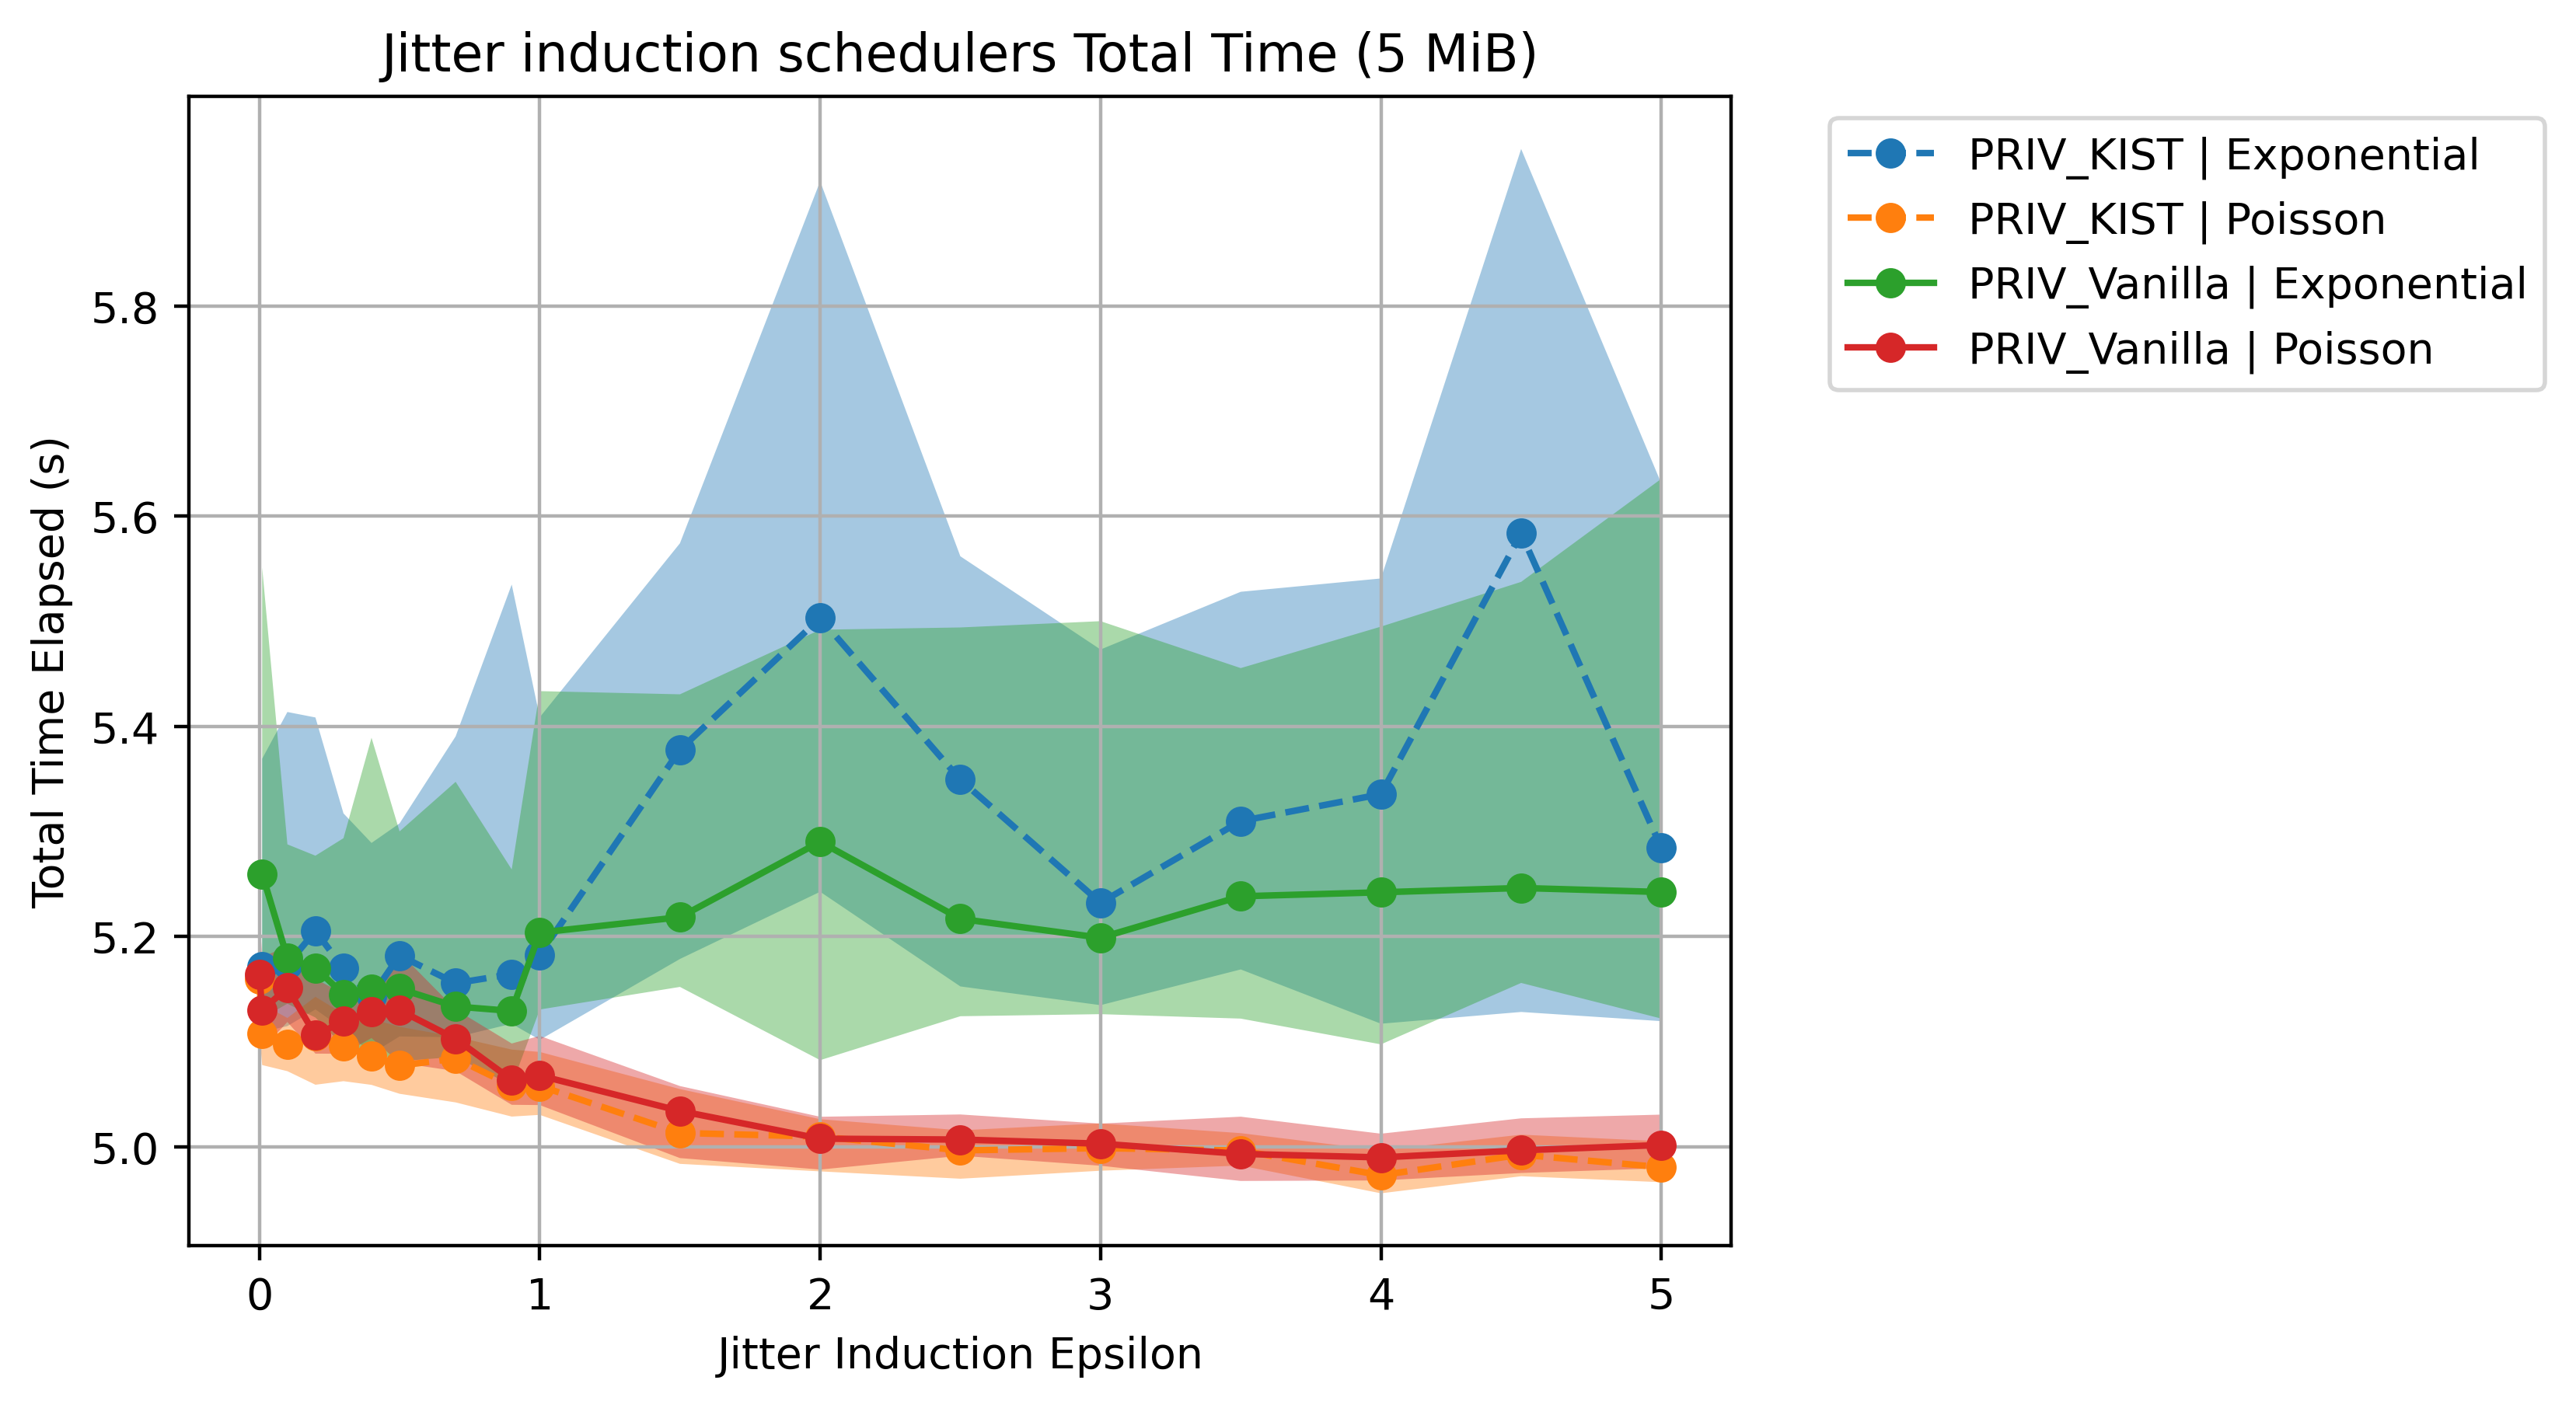
\includegraphics[width=\linewidth]{Chapters/Figures/Plots/local_total_time_50_jitter_5mib.png}}
    \end{subcaptionbox}
    \vfill
    \begin{subcaptionbox}{Both Features\label{fig:local_both_total_time}}[0.70\textwidth]
        {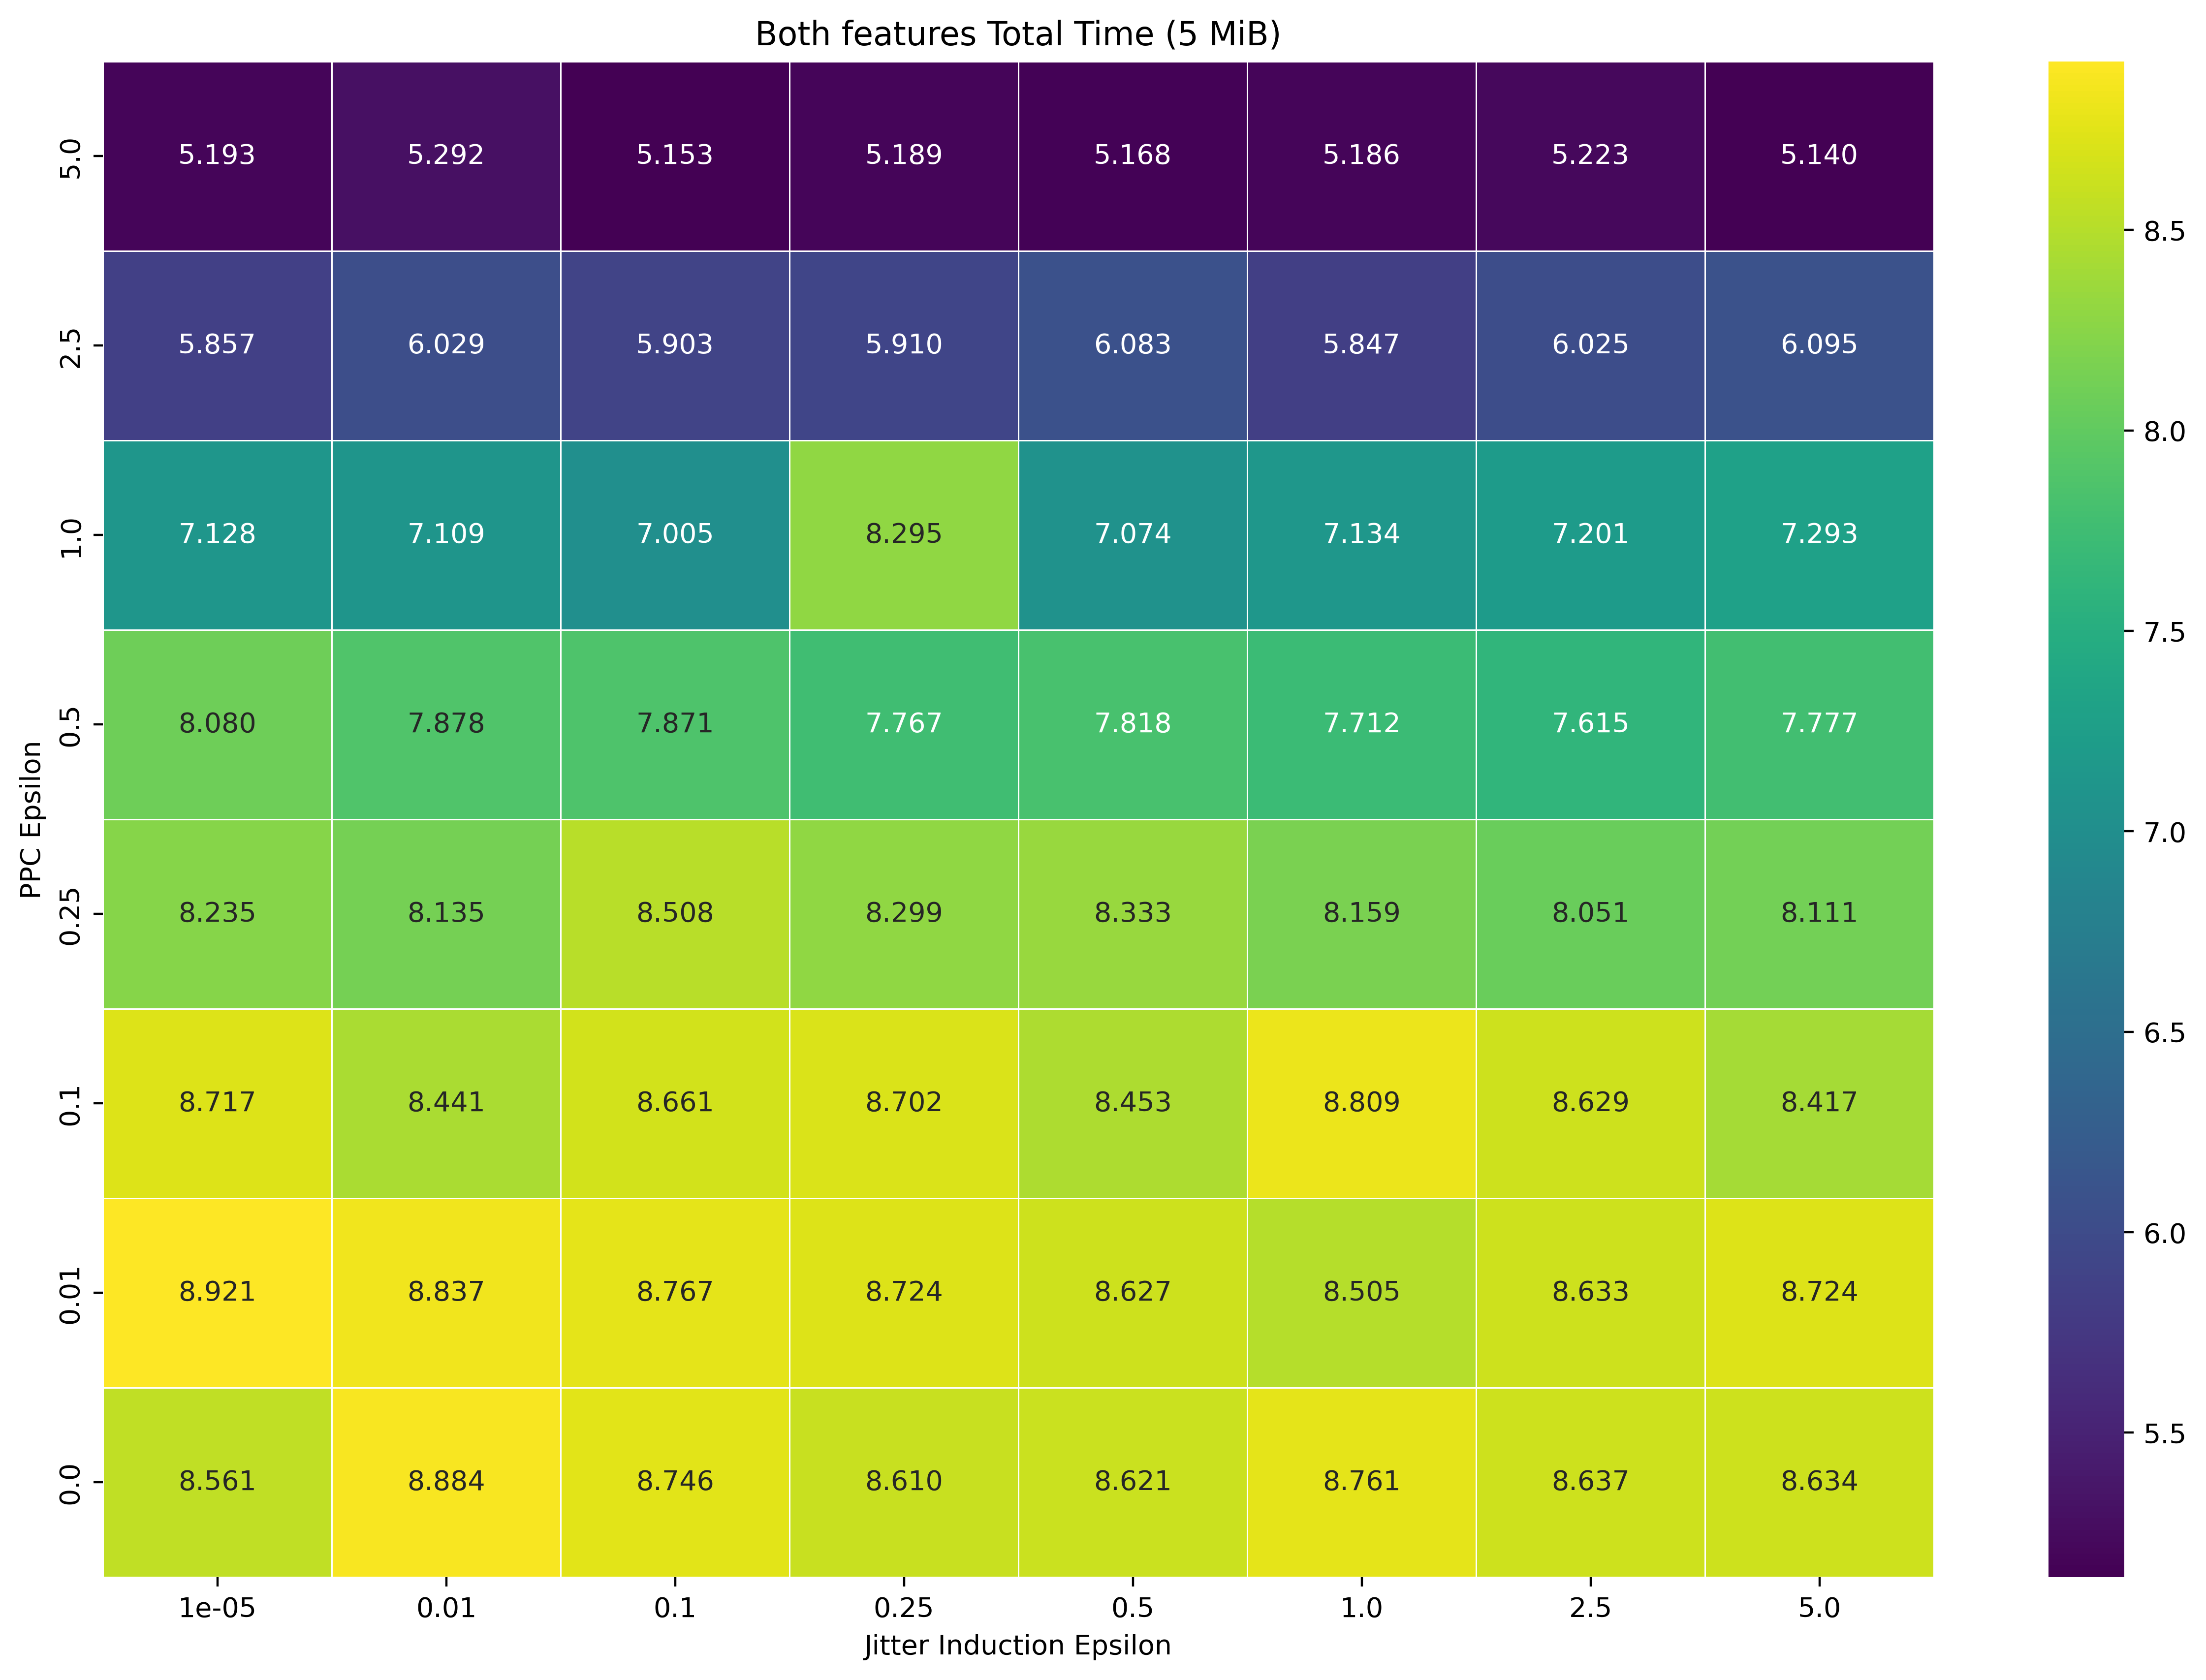
\includegraphics[width=\linewidth]{Chapters/Figures/Plots/local_total_time_50_heatmap_5mib.png}}
    \end{subcaptionbox}
    \caption{Total Time Results on Local Simulated Environment}\label{fig:local_total_time}
\end{figure}

\begin{figure}[htbp]
    \centering
    \begin{subcaptionbox}{Only Packet Padding Cells Feature\label{fig:dist_ppc_total_time}}[0.45\textwidth]
        {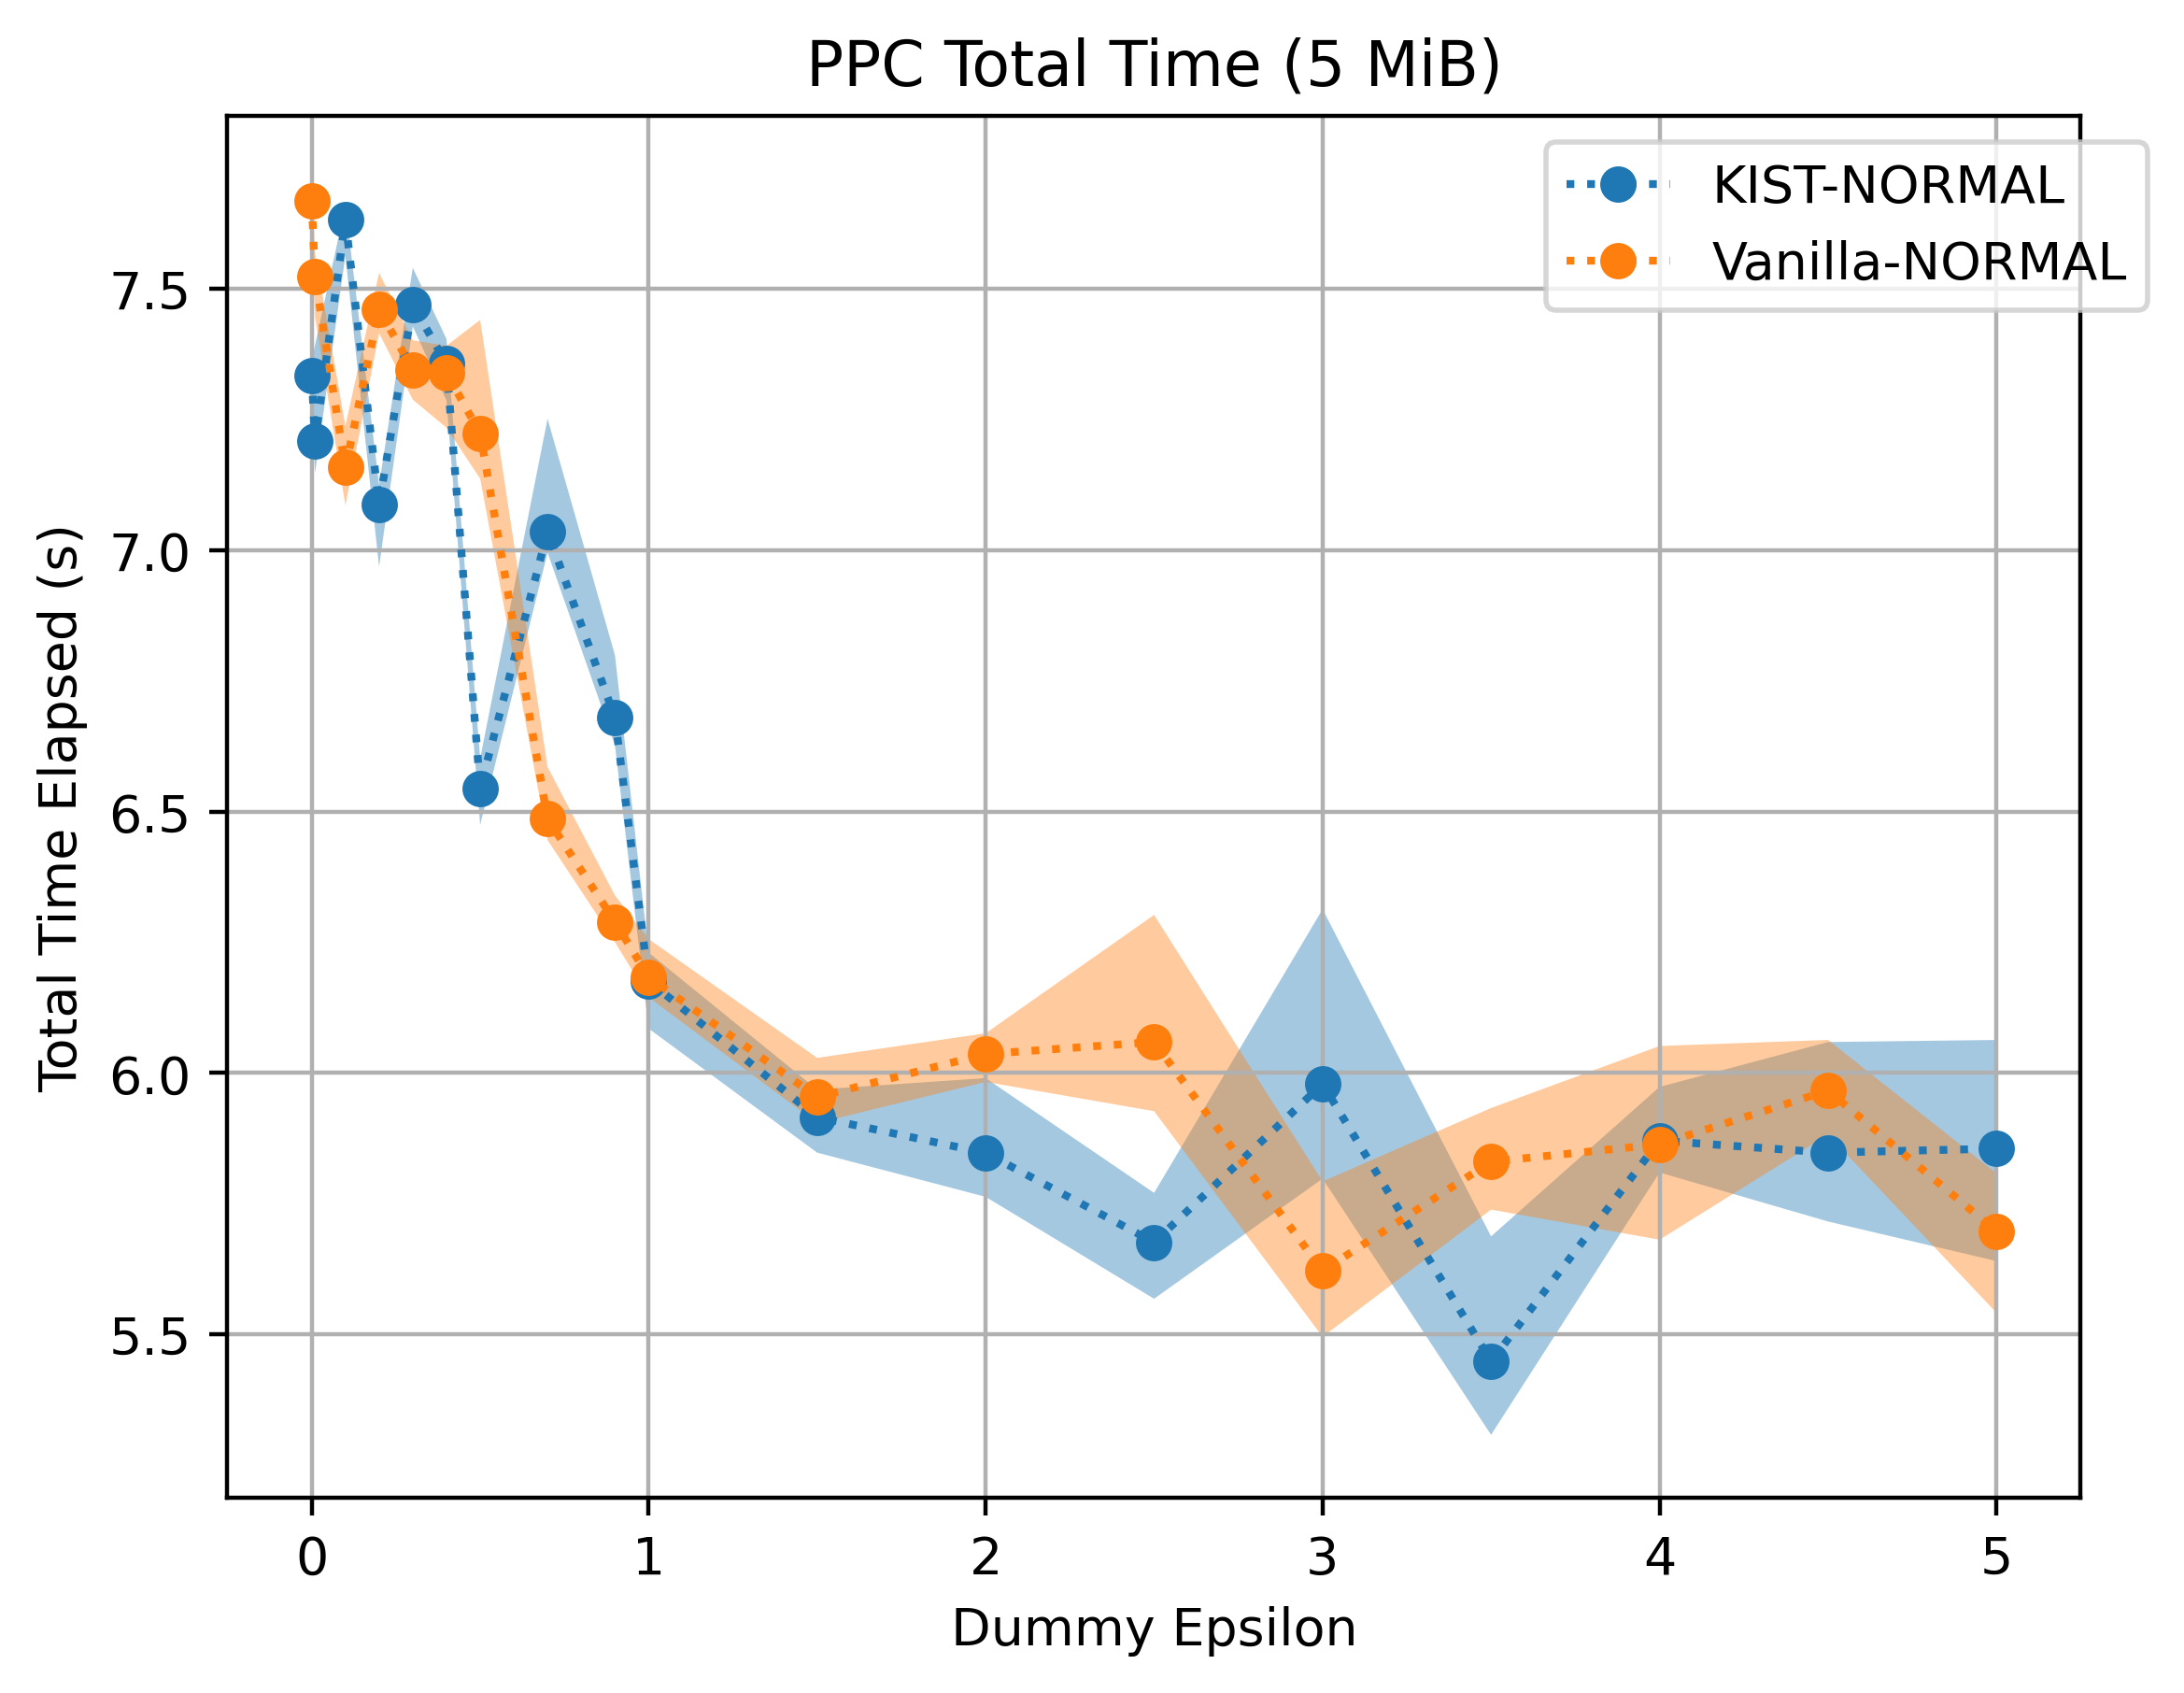
\includegraphics[width=\linewidth]{Chapters/Figures/Plots/dist_total_time_50_PPC_5mib.png}}
    \end{subcaptionbox}
    \hfill
    \begin{subcaptionbox}{Only Jitter Injection Schedulers Feature\label{fig:dist_jitter_total_time}}[0.45\textwidth]
        {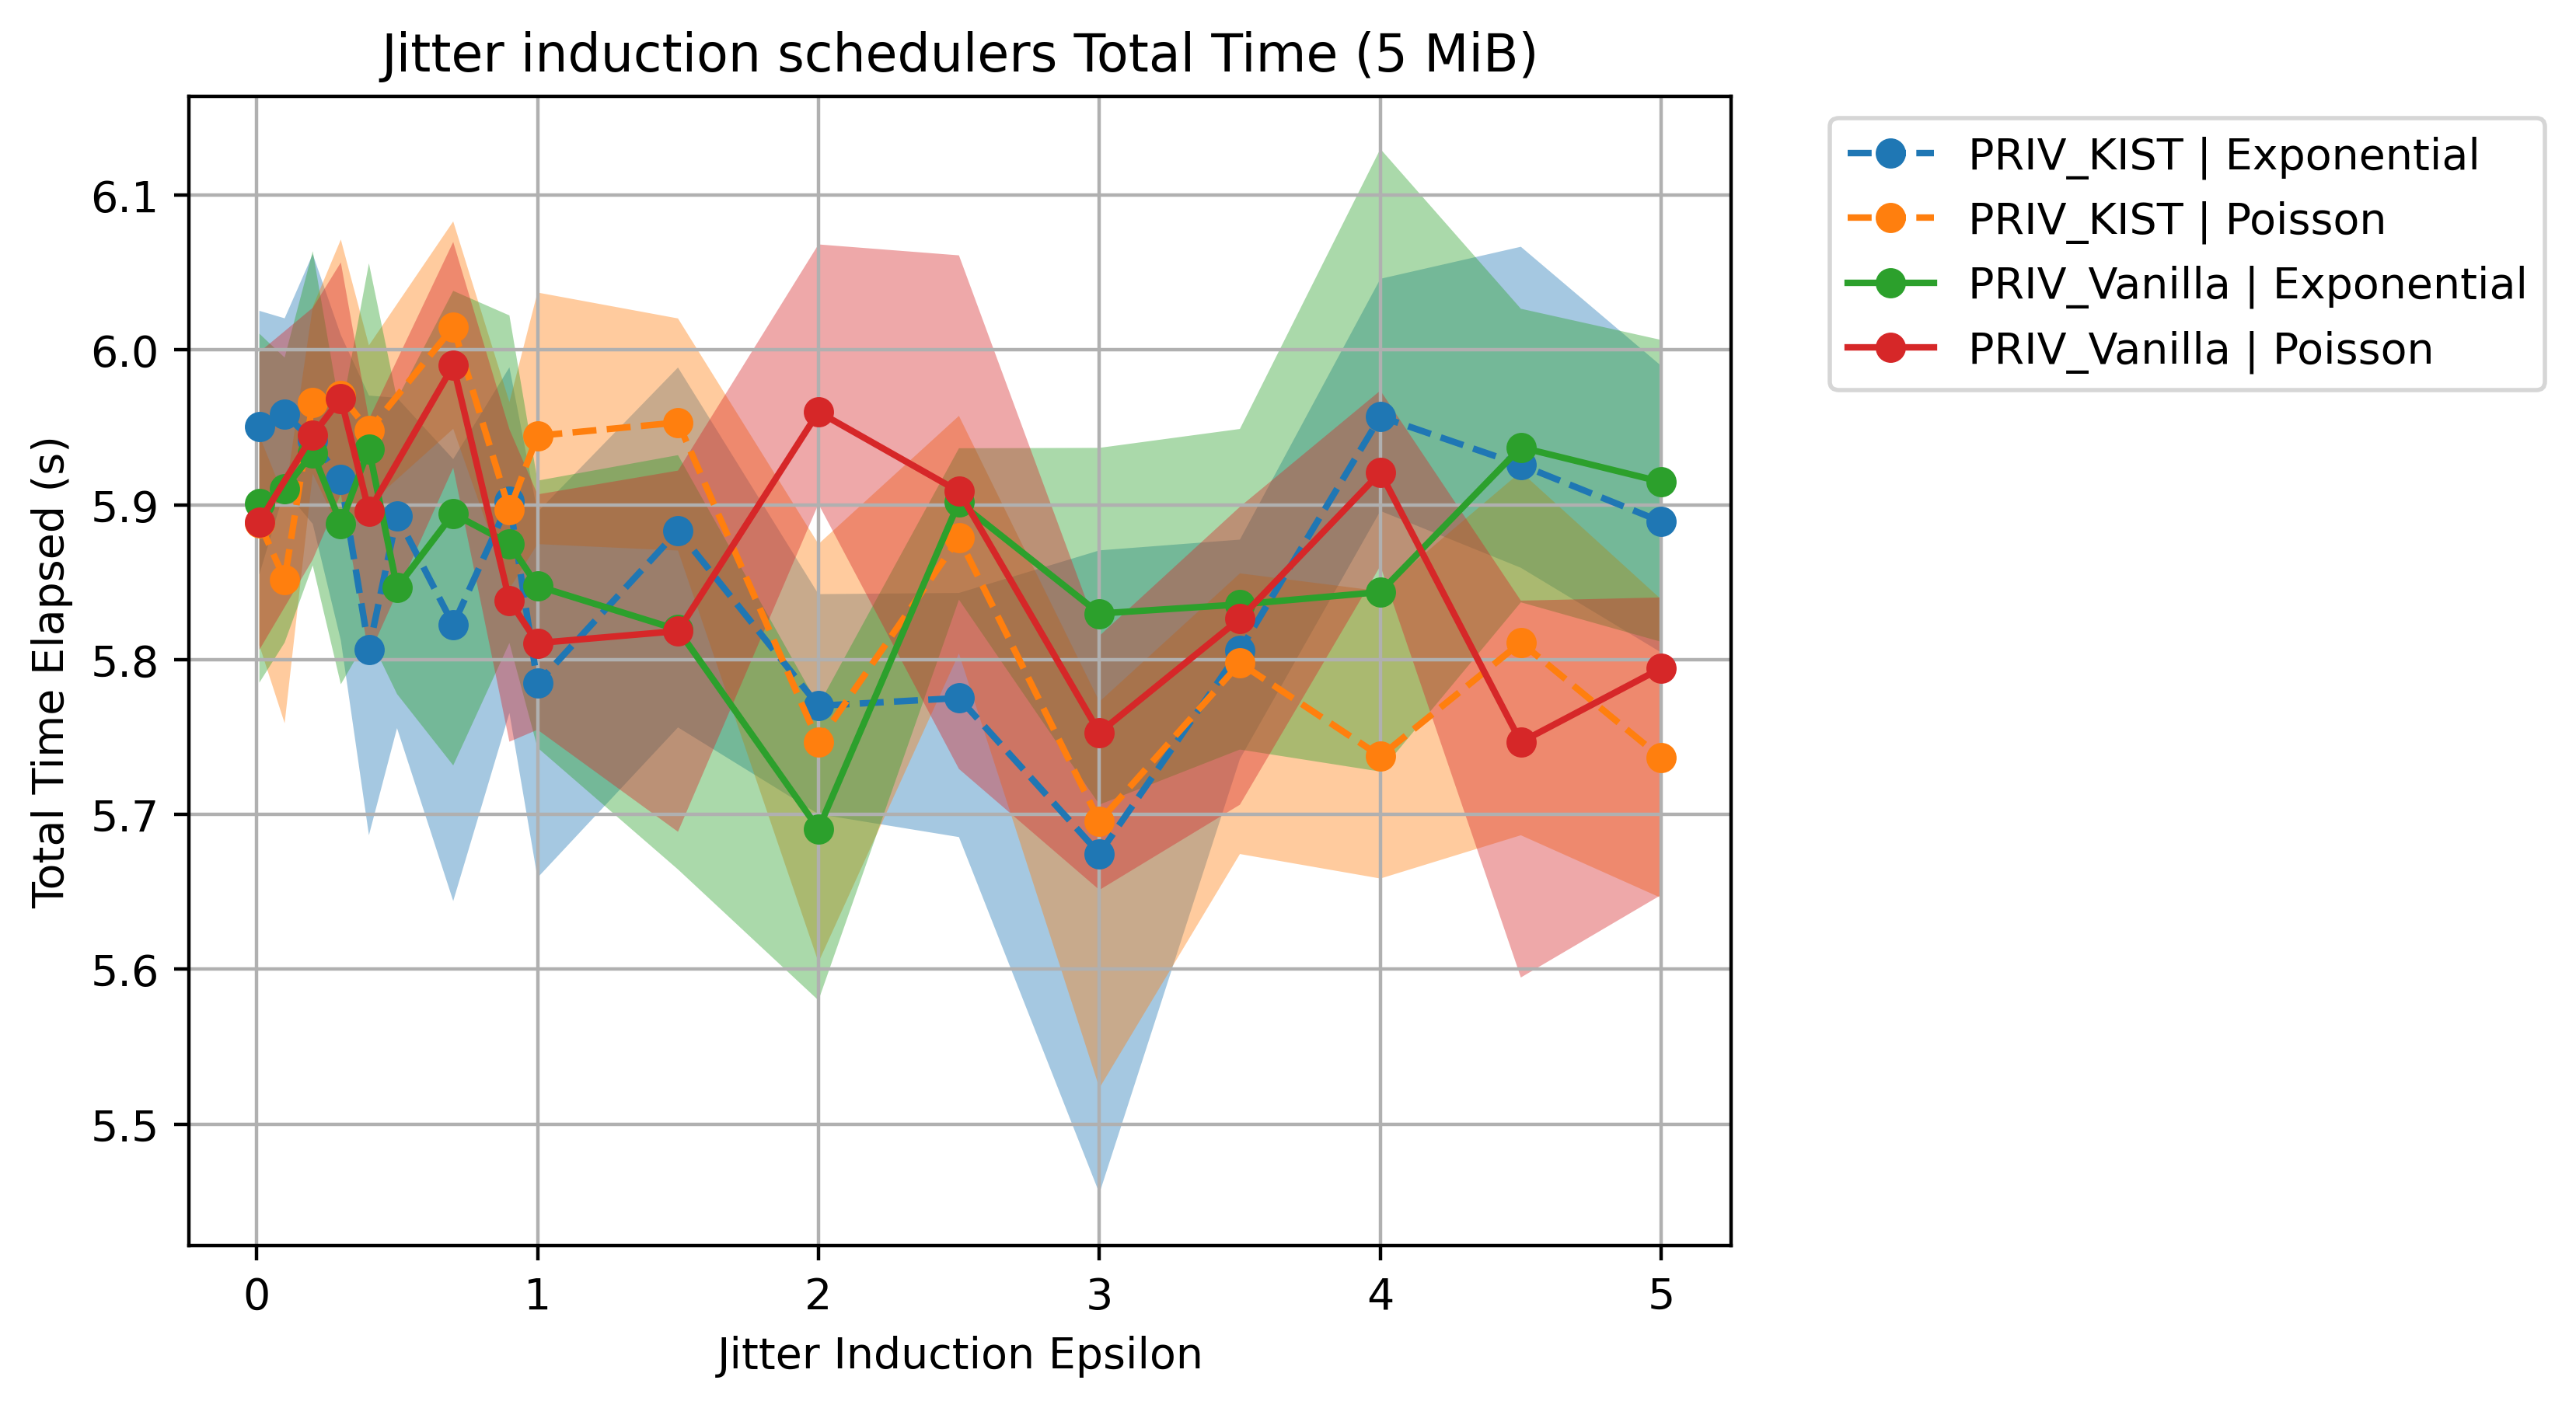
\includegraphics[width=\linewidth]{Chapters/Figures/Plots/dist_total_time_50_jitter_5mib.png}}
    \end{subcaptionbox}
    \vfill
    \begin{subcaptionbox}{Both Features\label{fig:dist_both_total_time}}[0.70\textwidth]
        {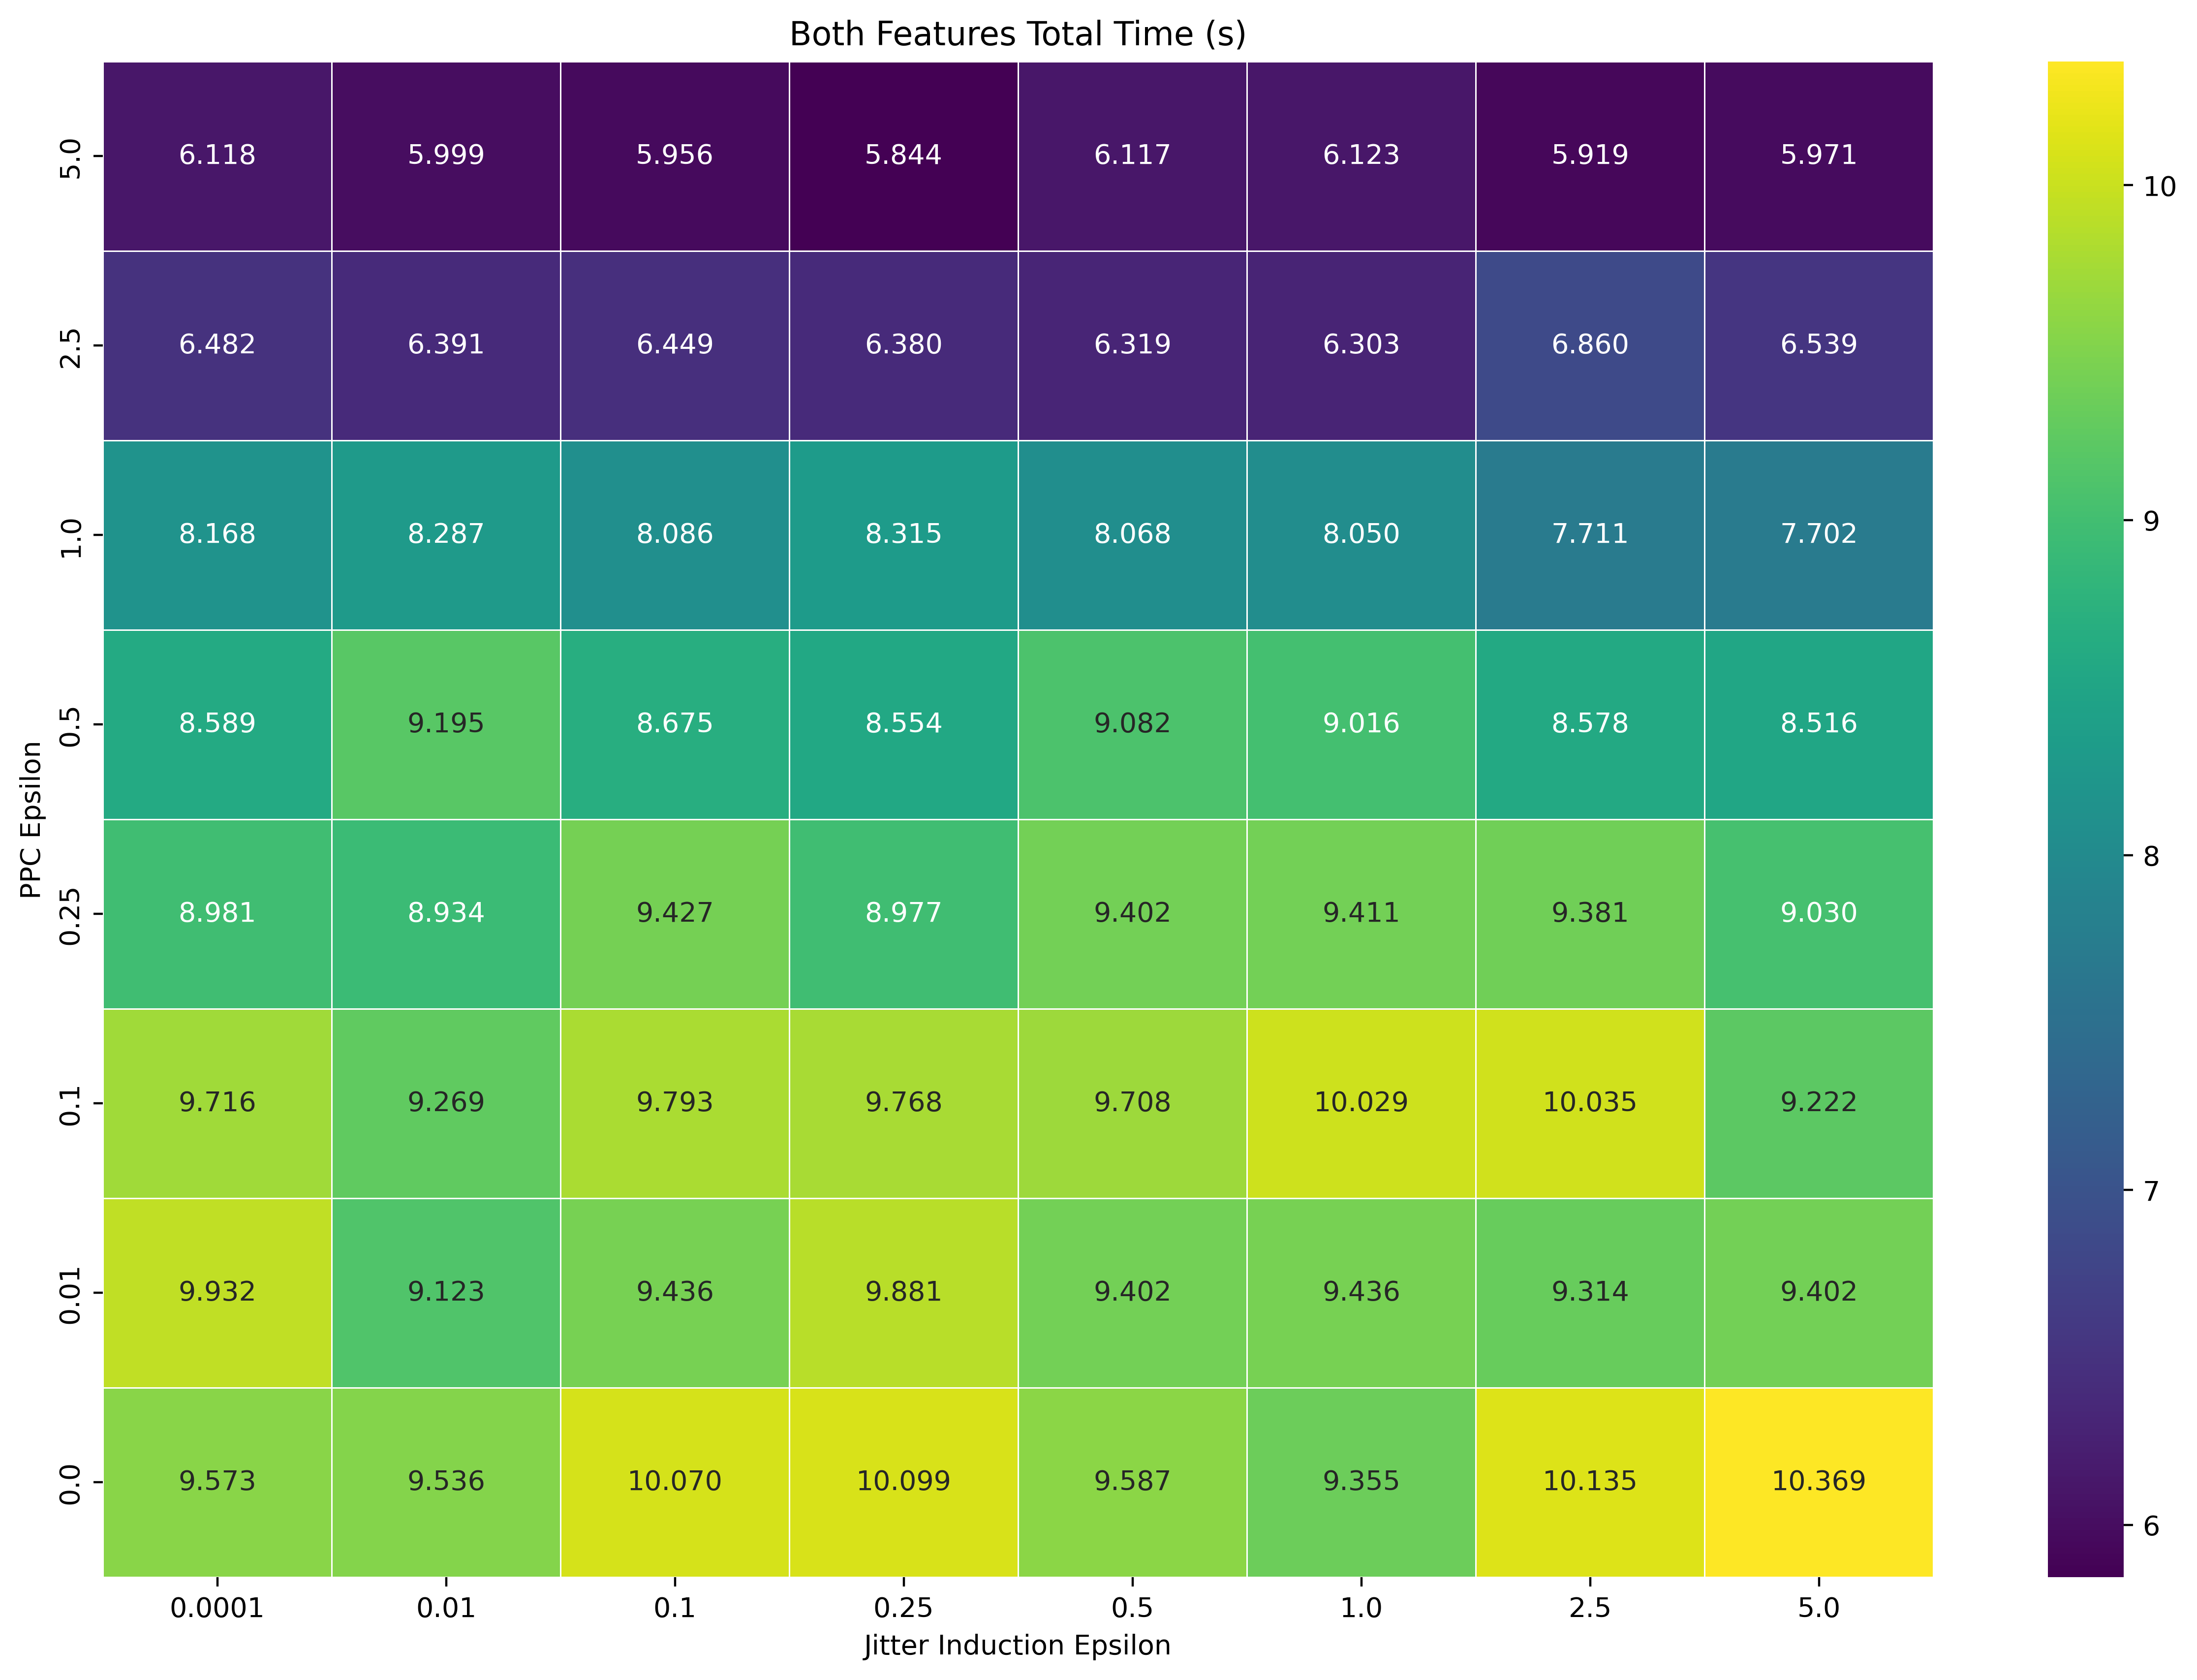
\includegraphics[width=\linewidth]{Chapters/Figures/Plots/dist_total_time_50_heatmap_5mib.png}}
    \end{subcaptionbox}
    \caption{Total Time Results on Distributed Environment}\label{fig:dist_total_time}
\end{figure}

As demonstrated in~\autoref{fig:local_total_time} and~\autoref{fig:dist_total_time}, the total time to download a file got results proportional to the throughput results, meaning that the PPC feature significantly influenced the total time to download. Regarding the Packet Padding Cells feature, the total time experienced is significantly lower as $\epsilon_{PPC}$ decreases. The same can be said about the Schedulers feature, although the impact is smaller. Additionally, the Exponential distribution showed a higher variance in the local test bench, and the median results unexpectably increased 0.1 seconds. This situation got normalized in the distributed test bench.   
Both schedulers behaved similarly in all experiments, thus we used the KIST variant and the Poisson distribution to test both features together. The results of the combined features also emphasized the greater impact of the PPC feature on the total time to download a file. Alike the throughput results, the total time heatmap proves that the schedulers feature has a negligible impact on the total time, when compared with the PPC.\@
%TODO: MUST TEST COMBINATIONS ON DISTRIBUTED TO GET BETTER ANALYSIS ON WORSE/BETTER TEST BENCH AND CONFIGURATION
\begin{table}[htbp]
    \centering
    \begin{tabular}{|c|c|c|}
    \hline
    \textbf{Configuration} & \textbf{Local} & \textbf{Distributed} \\
    \hline
    Tor Metrics &  \multicolumn{2}{c|}{4.825} \\ 
    \hline
    \multirow{2}{*}{Control} & 5.09 & 5.95\\ 
    & 5.09 & 5.75\\
    \hline
    Only PPC & 5.02 – 8.07 & 5.45 – 7.67\\
    \hline
    Only Jitter & 5.58 – 4.97 & 5.67 – 6.01\\
    \hline
    PPC \& Jitter & 5.13 – 8.88 & 5.87 – 6.32\\
    \hline
    \end{tabular}
    \caption{Total Time Results Summary (s)}\label{tab:total_time_summary}
\end{table}

\FloatBarrier
\subsection{Latency}

Tor Metrics defines their circuit round-trip latencies as the time between the HTTP request and the first byte of the HTTP response's header. This way, we obtained the latency results based on the time to the first byte of the HTTP response's header. This metric also represents a key aspect of a communication system such as Tor because it allows to understand the maximum rate information may be transmitted. 

Similarly to the previous metrics, we present the latency results obtained from our experiments in~\autoref{fig:local_latency} for the local simulated environment and~\autoref{fig:dist_latency} for the distributed environment. We followed the Tor Metrics directives and also present the results as a thick line which represents the median value, together with a shaded area representing the first and third quartiles.

\begin{figure}[htbp]
    \centering
    \begin{subcaptionbox}{Only Packet Padding Cells Feature\label{fig:local_ppc_latency}}[0.45\textwidth]
        {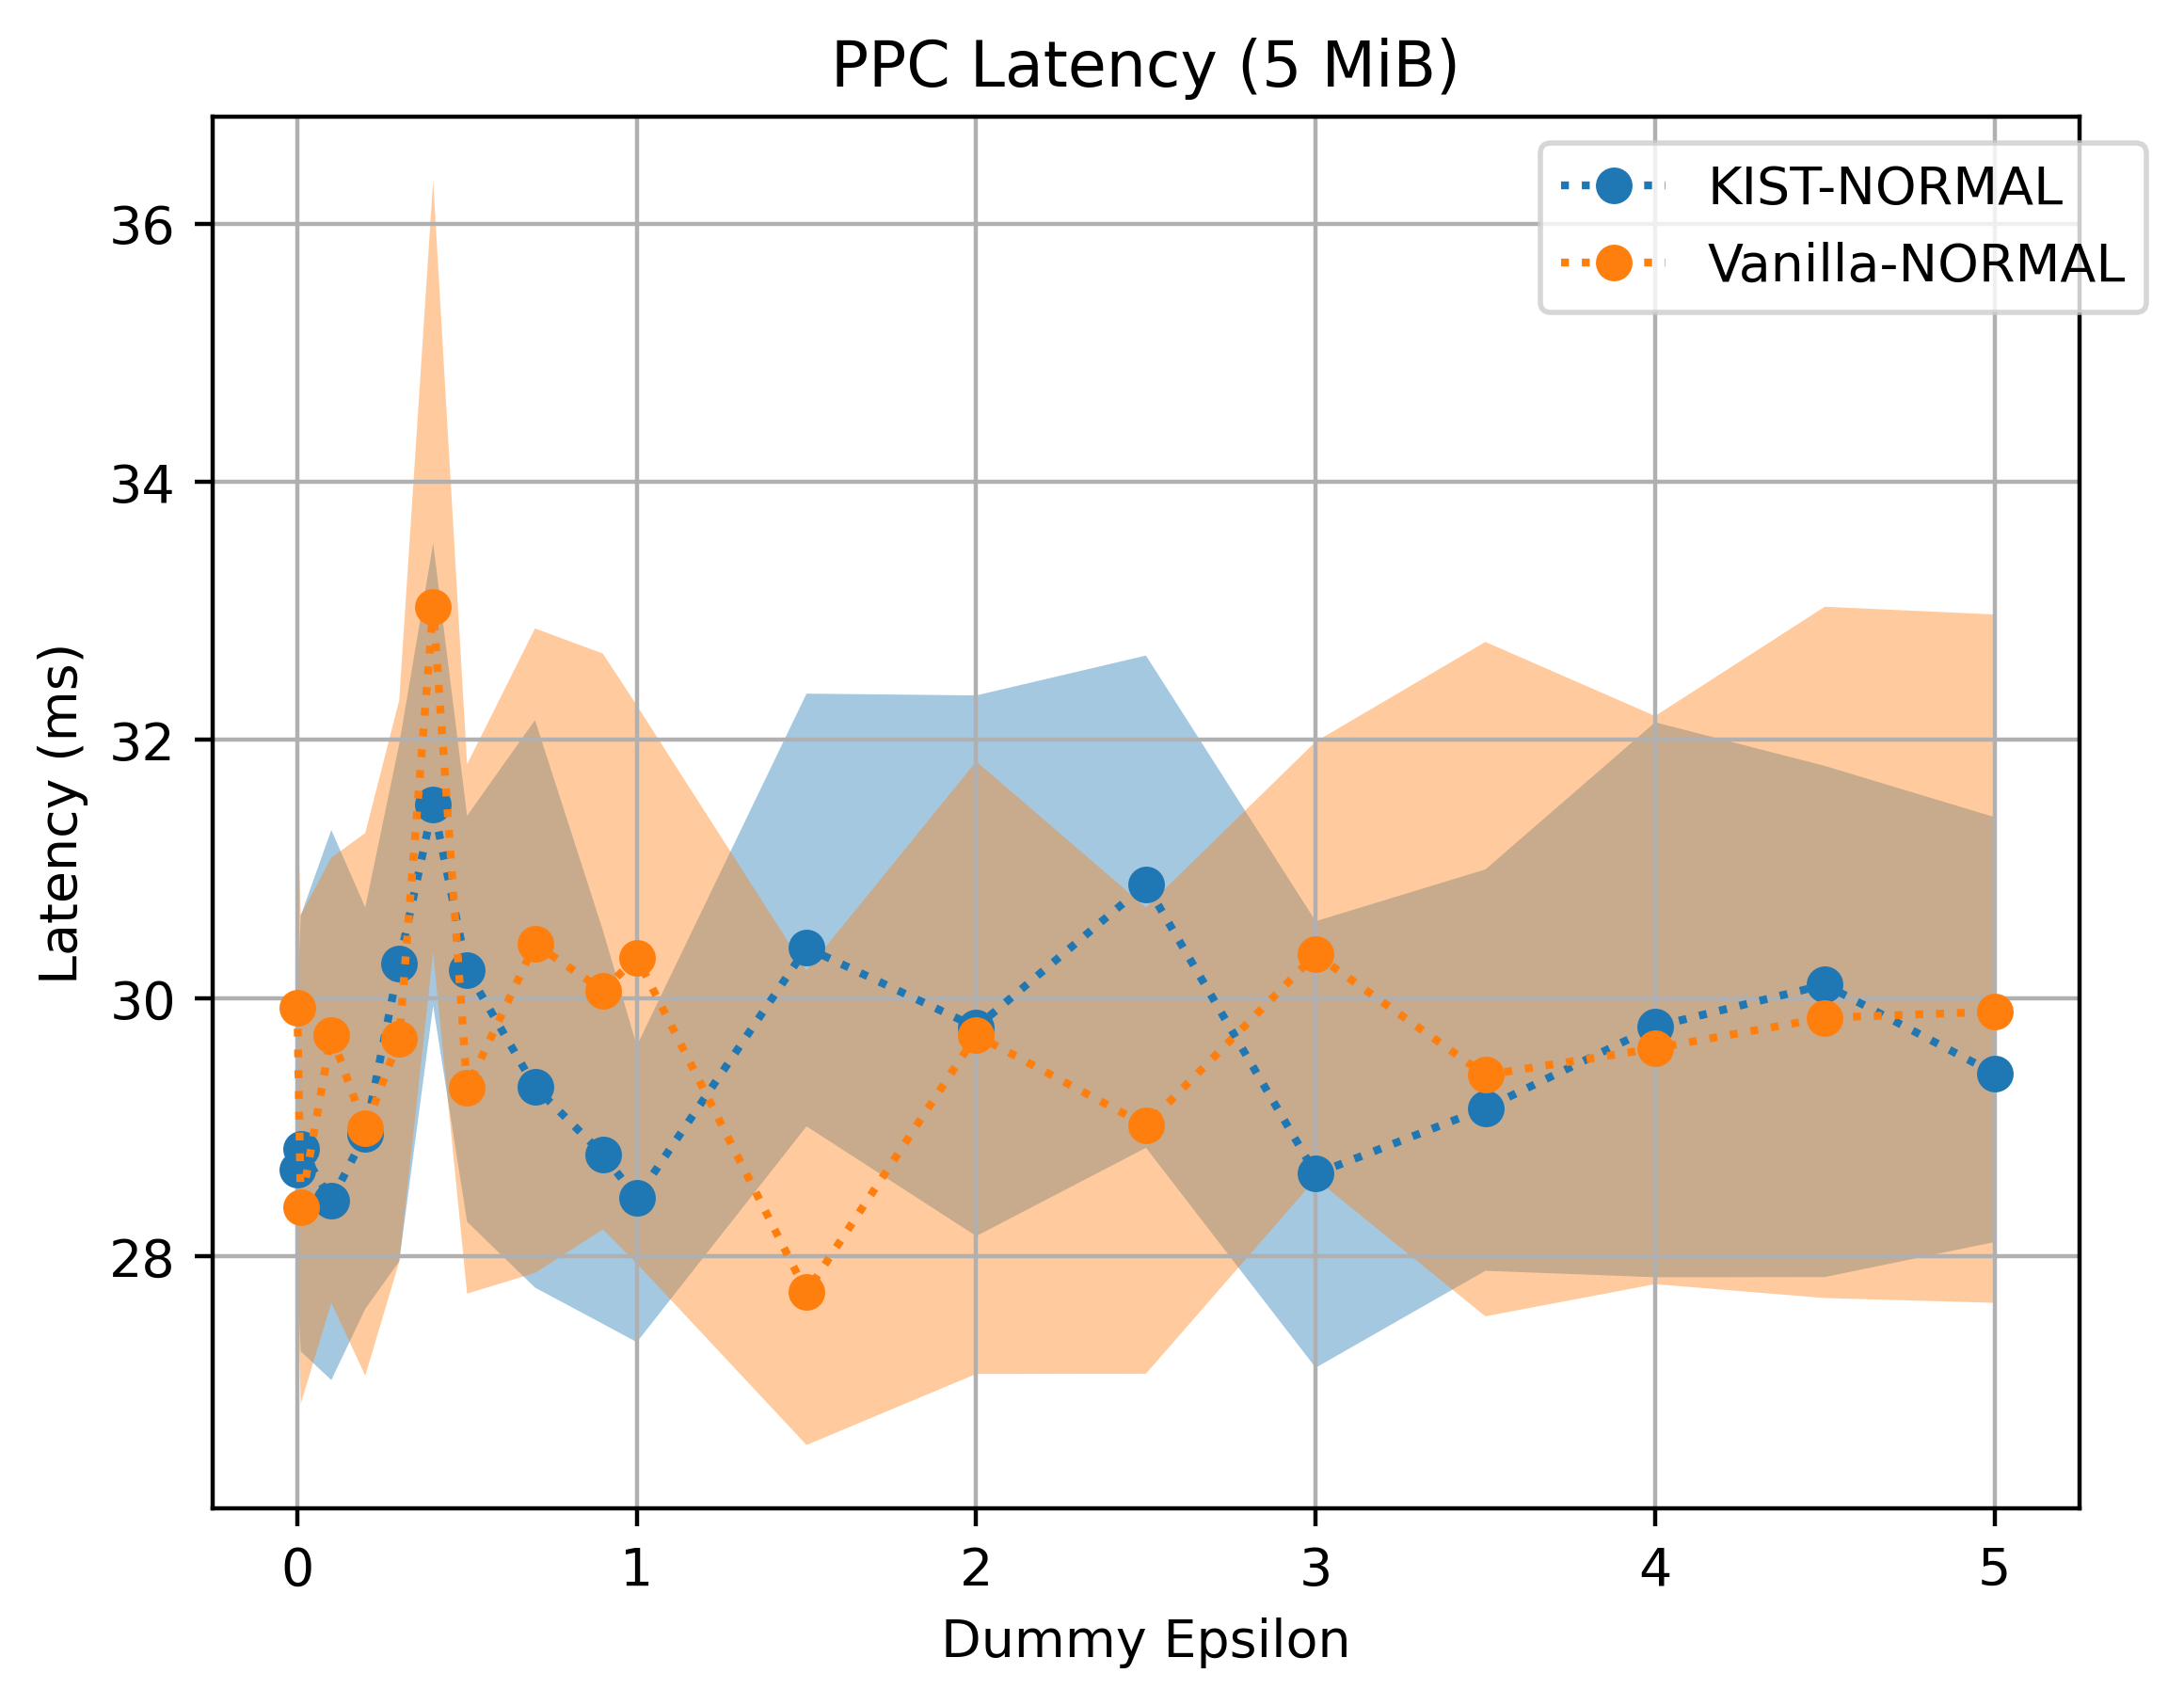
\includegraphics[width=\linewidth]{Chapters/Figures/Plots/local_latency_50_PPC_5mib.png}}
    \end{subcaptionbox}
    \hfill
    \begin{subcaptionbox}{Only Jitter Injection Schedulers Feature\label{fig:local_jitter_latency}}[0.45\textwidth]
        {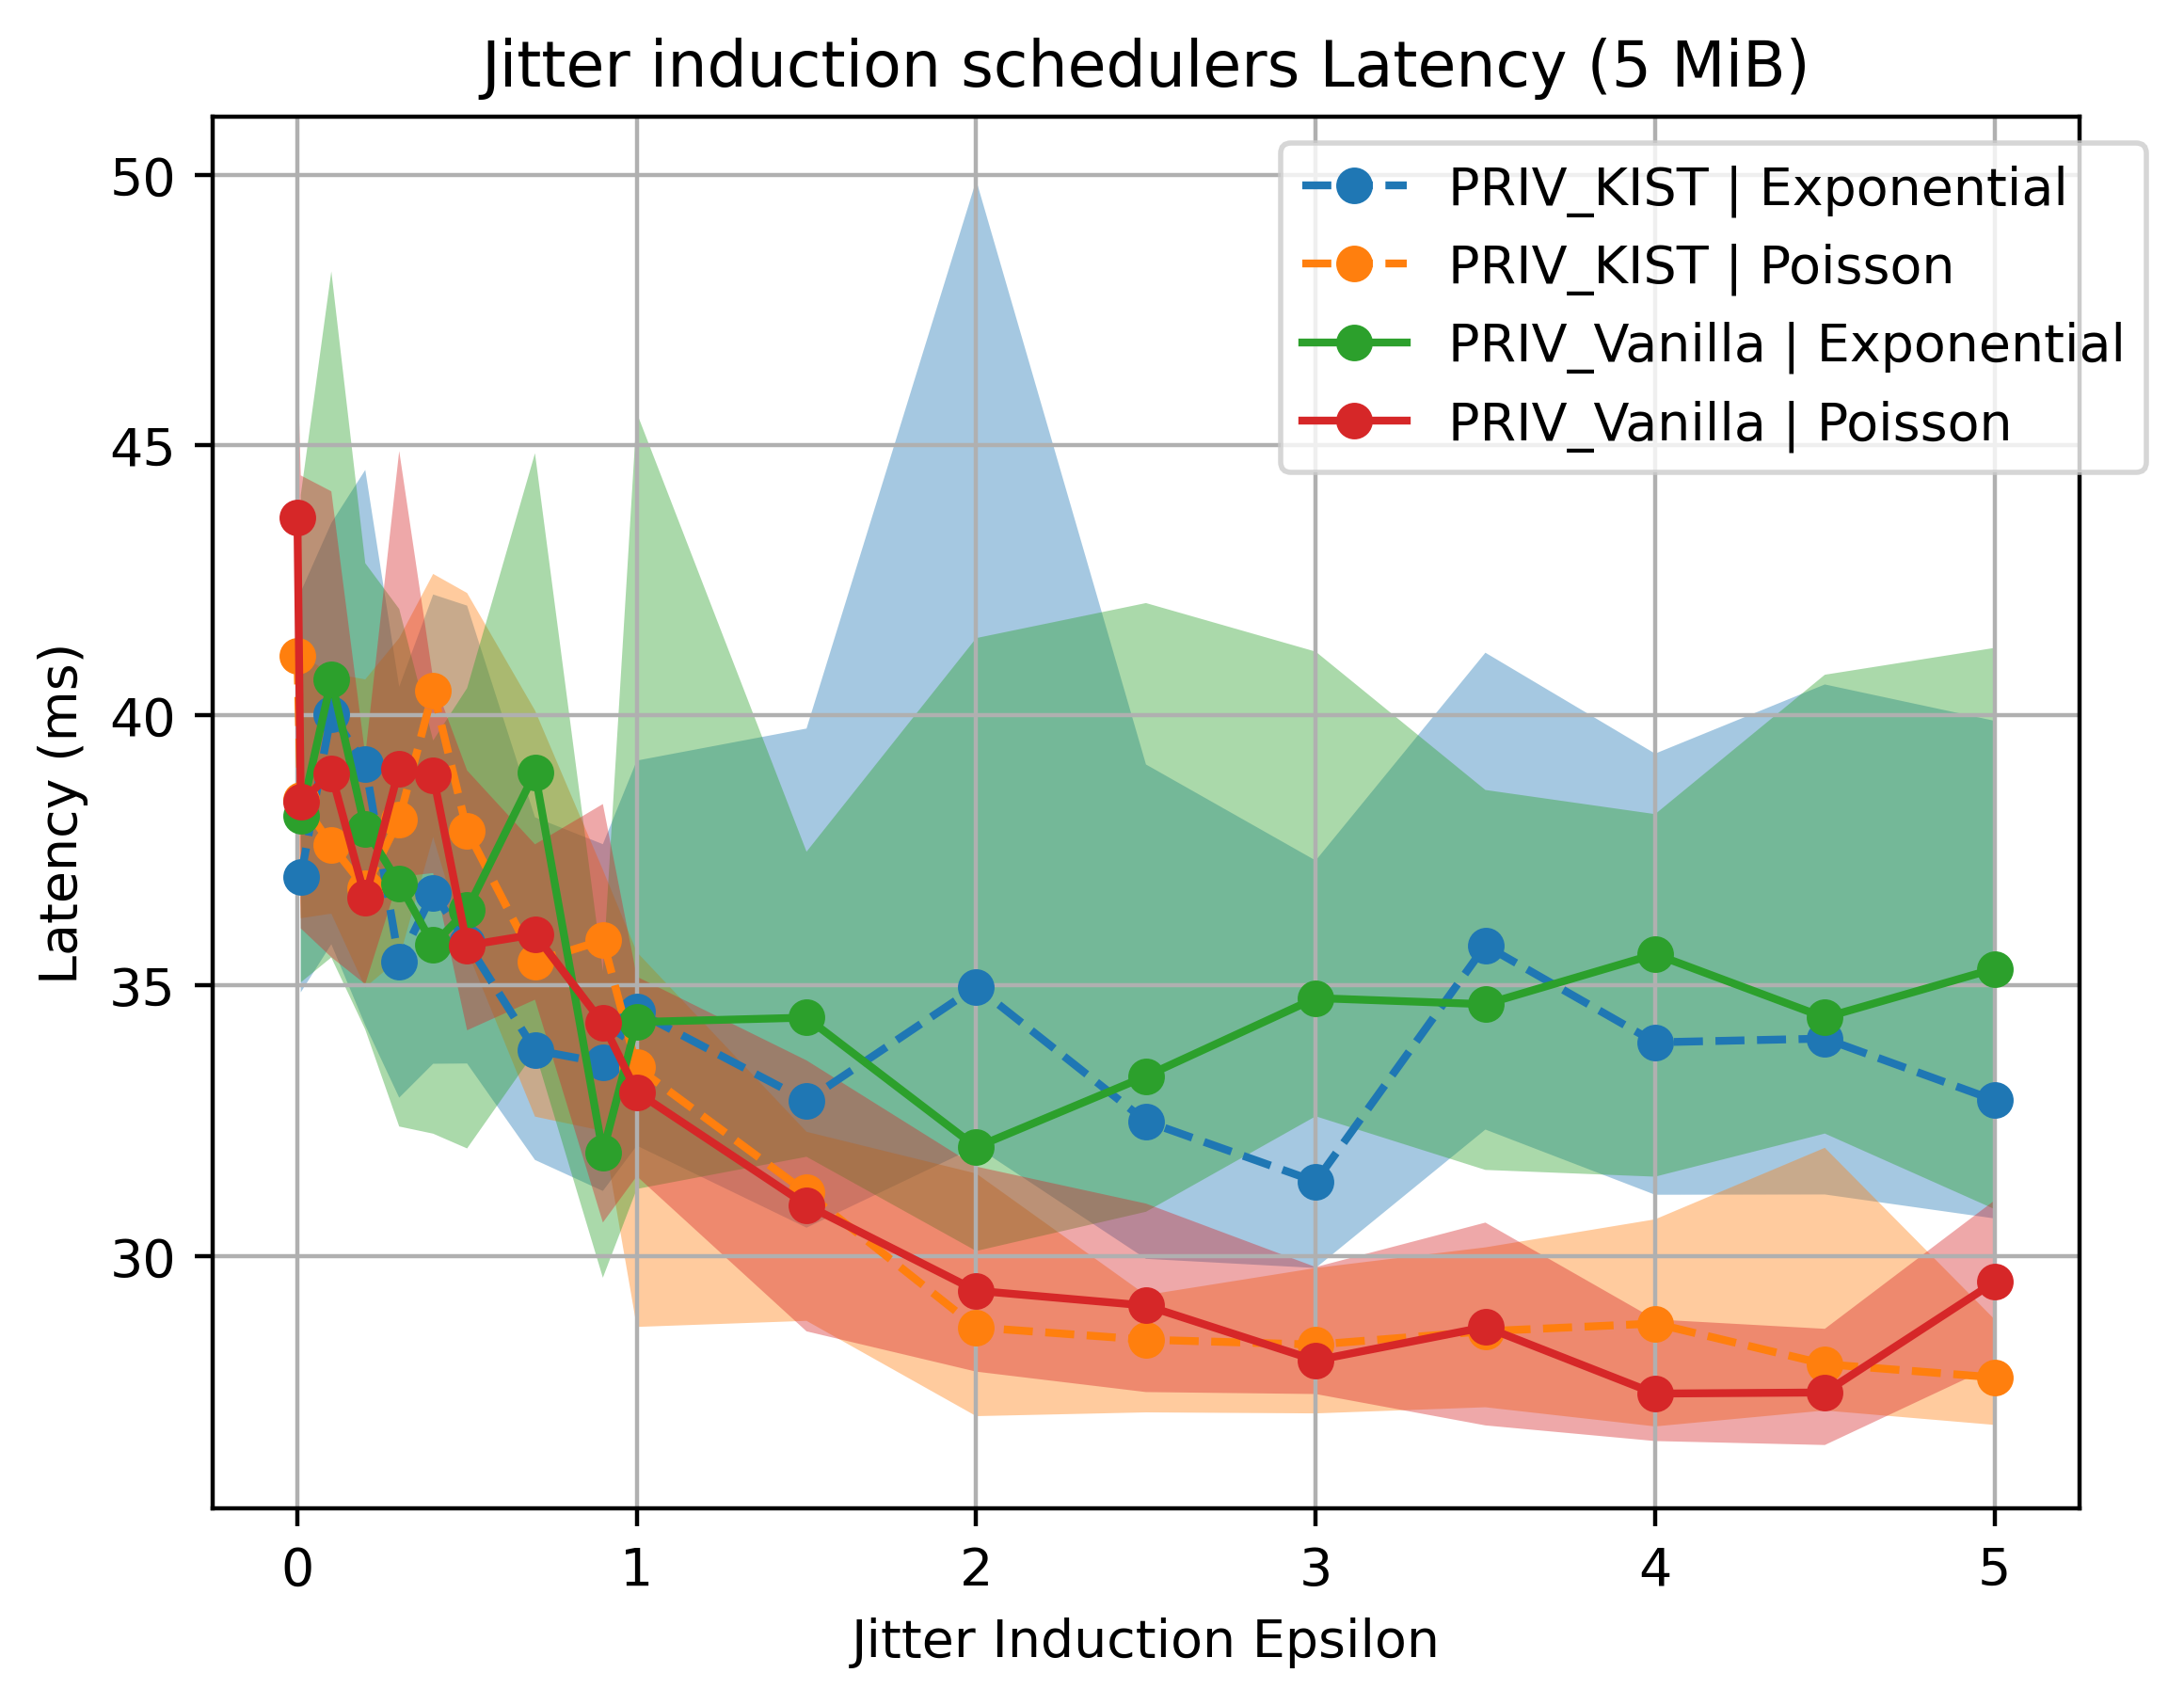
\includegraphics[width=\linewidth]{Chapters/Figures/Plots/local_latency_50_jitter_5mib.png}}
    \end{subcaptionbox}
    \vfill
    \begin{subcaptionbox}{Both Features\label{fig:local_both_latency}}[0.70\textwidth]
        {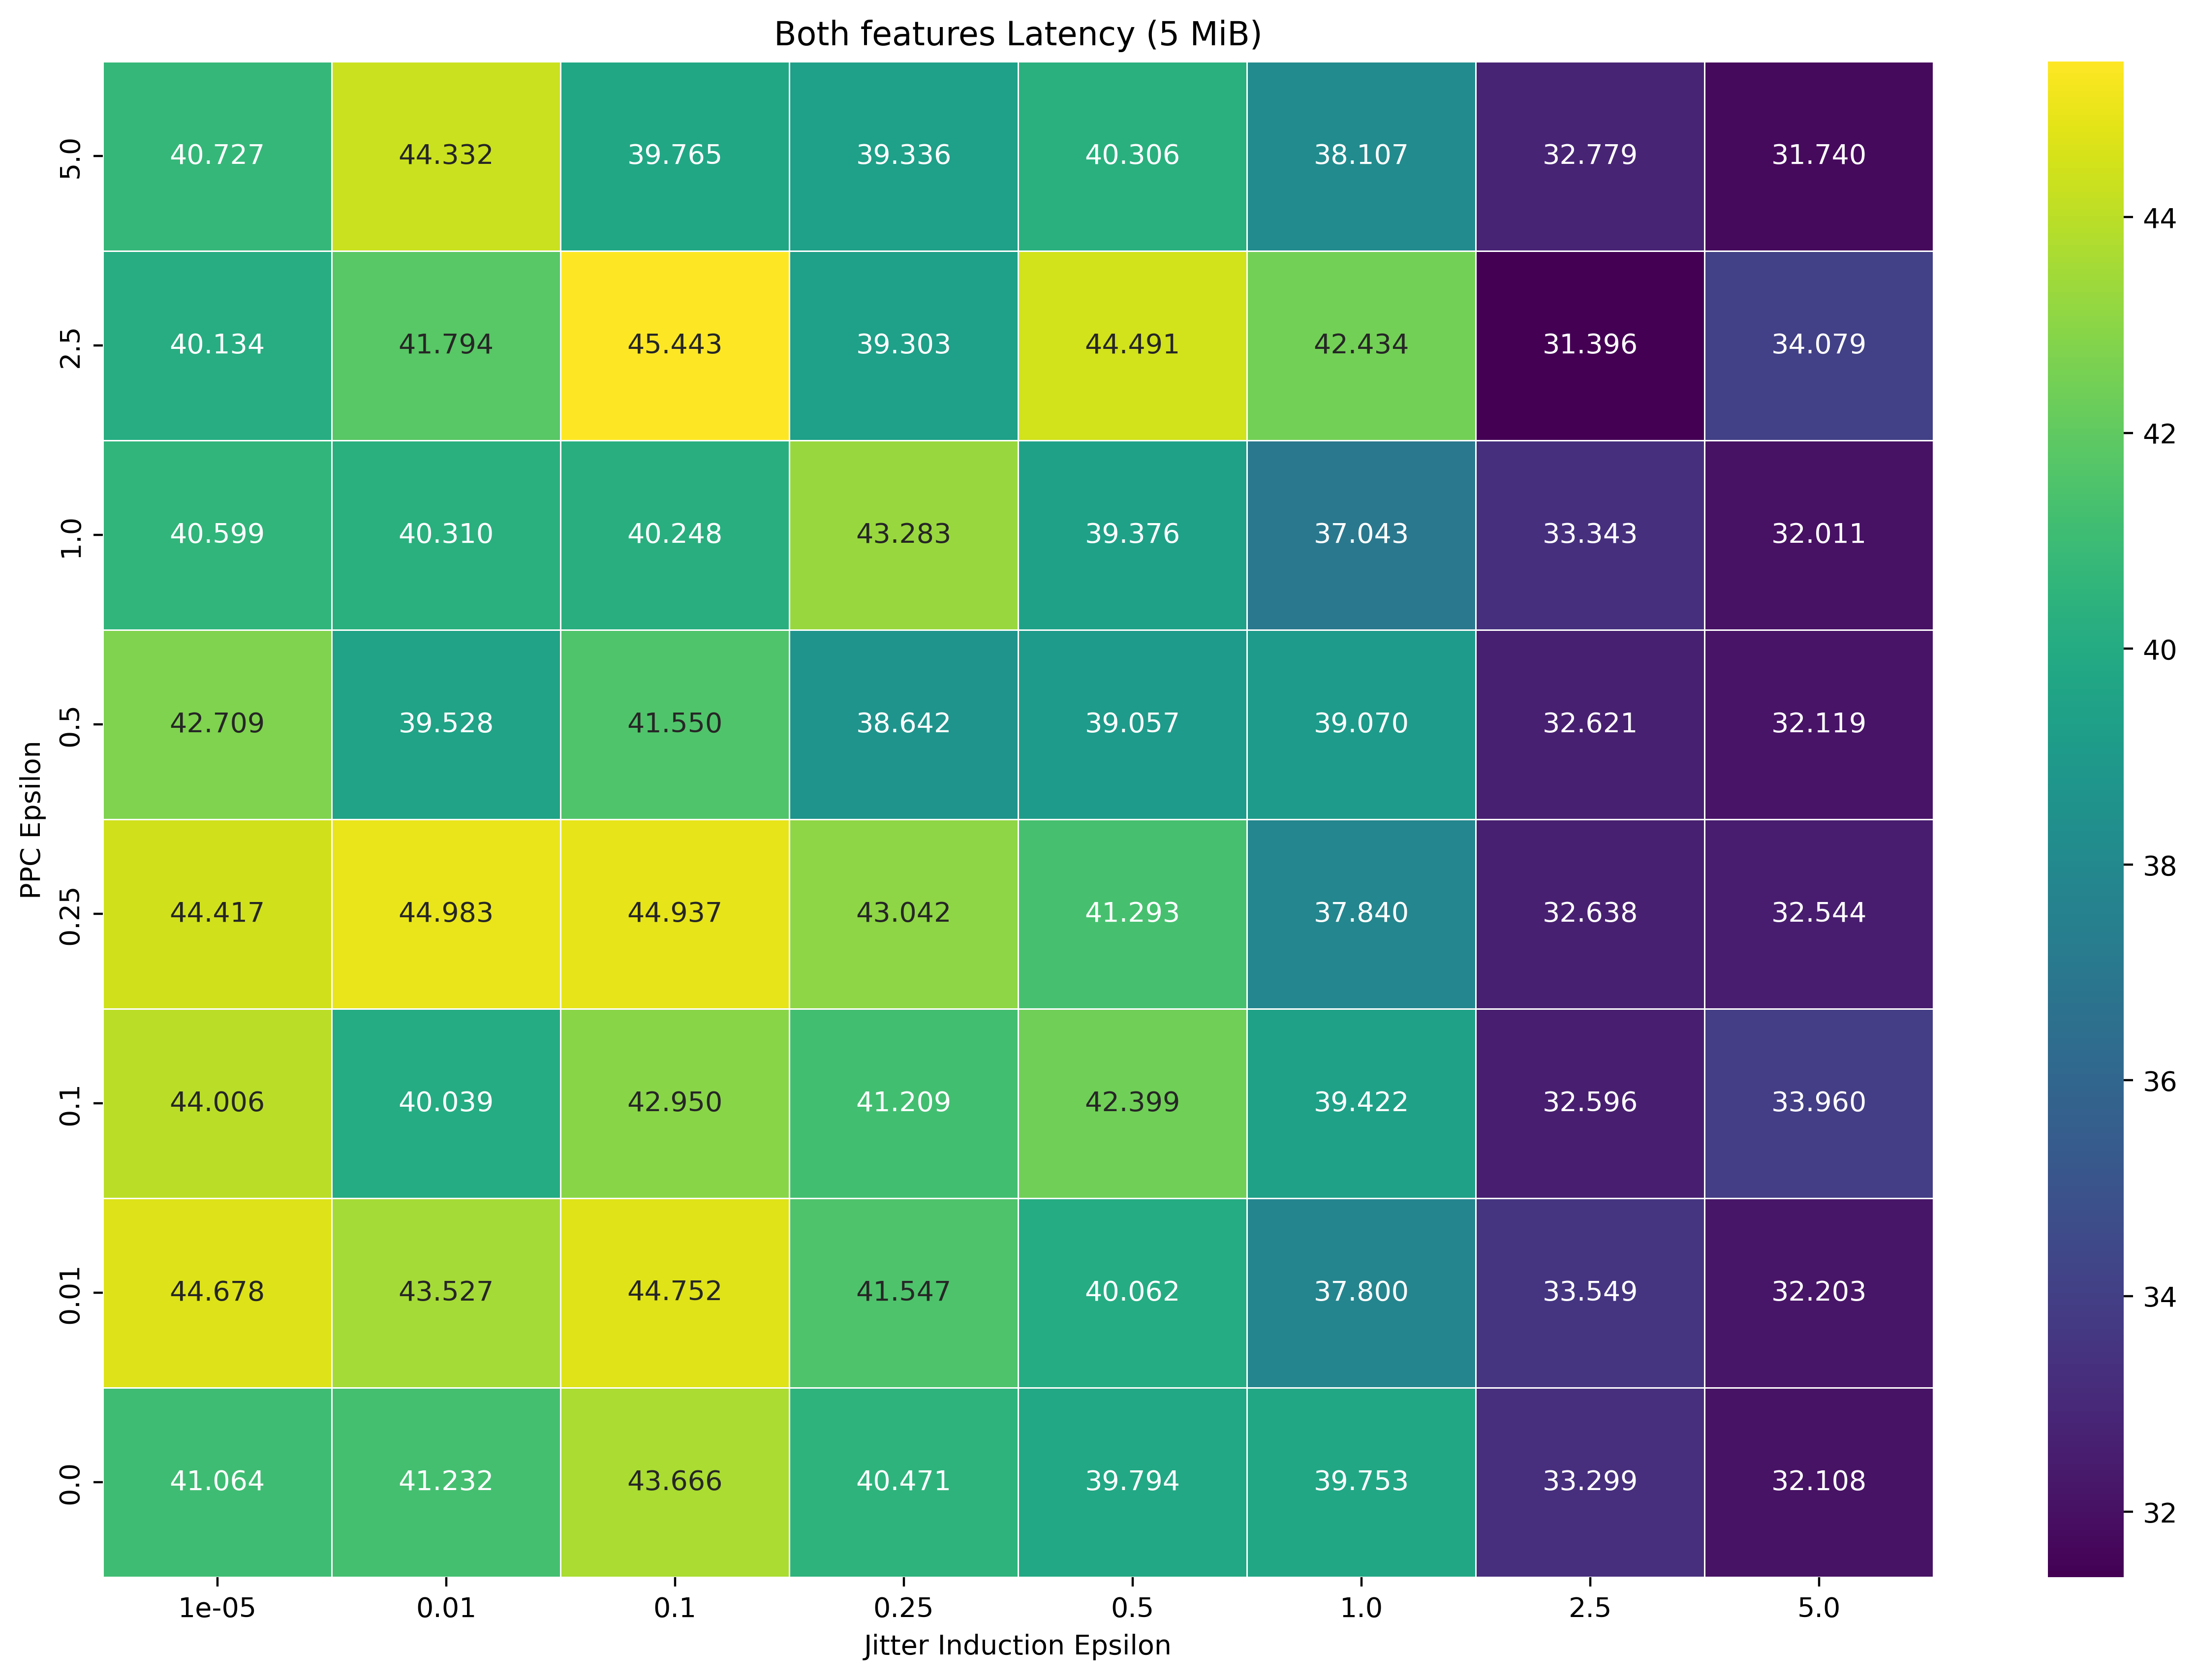
\includegraphics[width=\linewidth]{Chapters/Figures/Plots/local_latency_50_heatmap_5mib.png}}
    \end{subcaptionbox}
    \caption{Latency Results on Local Simulated Environment}\label{fig:local_latency}
\end{figure}

\begin{figure}[htbp]
    \centering
    \begin{subcaptionbox}{Only Packet Padding Cells Feature\label{fig:dist_ppc_latency}}[0.45\textwidth]
        {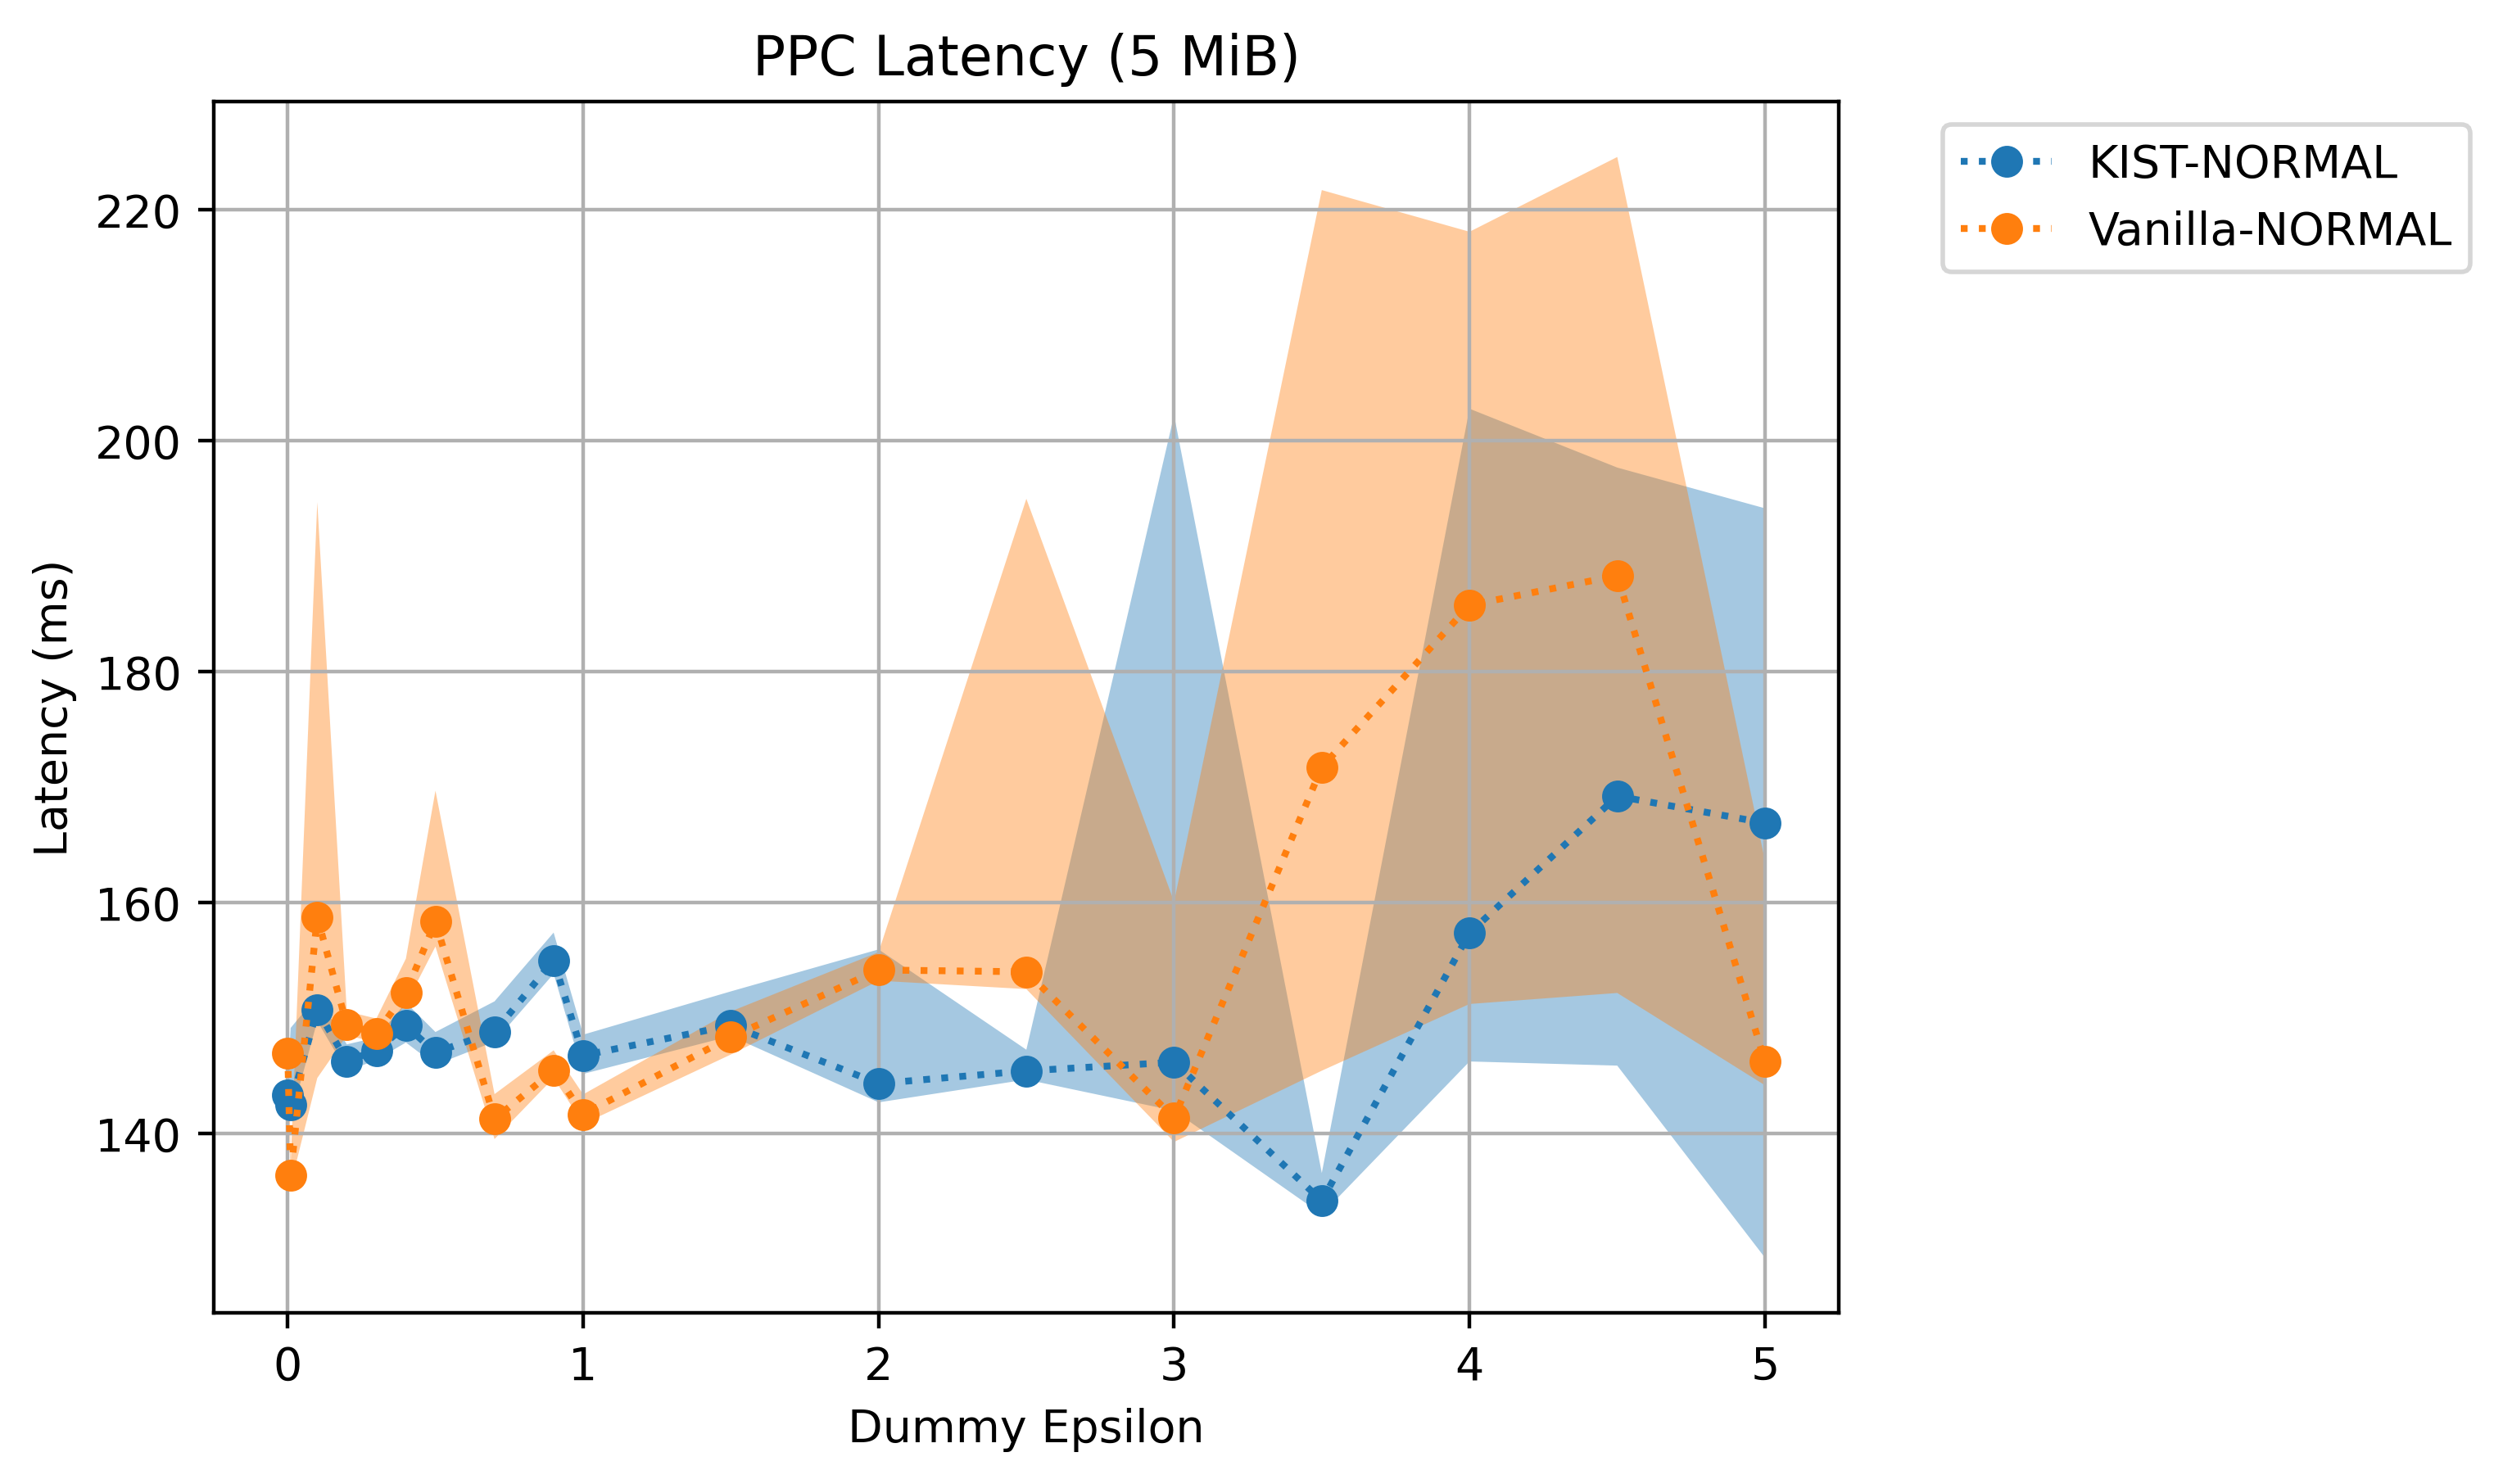
\includegraphics[width=\linewidth]{Chapters/Figures/Plots/dist_latency_50_PPC_5mib.png}}
    \end{subcaptionbox}
    \hfill
    \begin{subcaptionbox}{Only Jitter Injection Schedulers Feature\label{fig:dist_jitter_latency}}[0.45\textwidth]
        {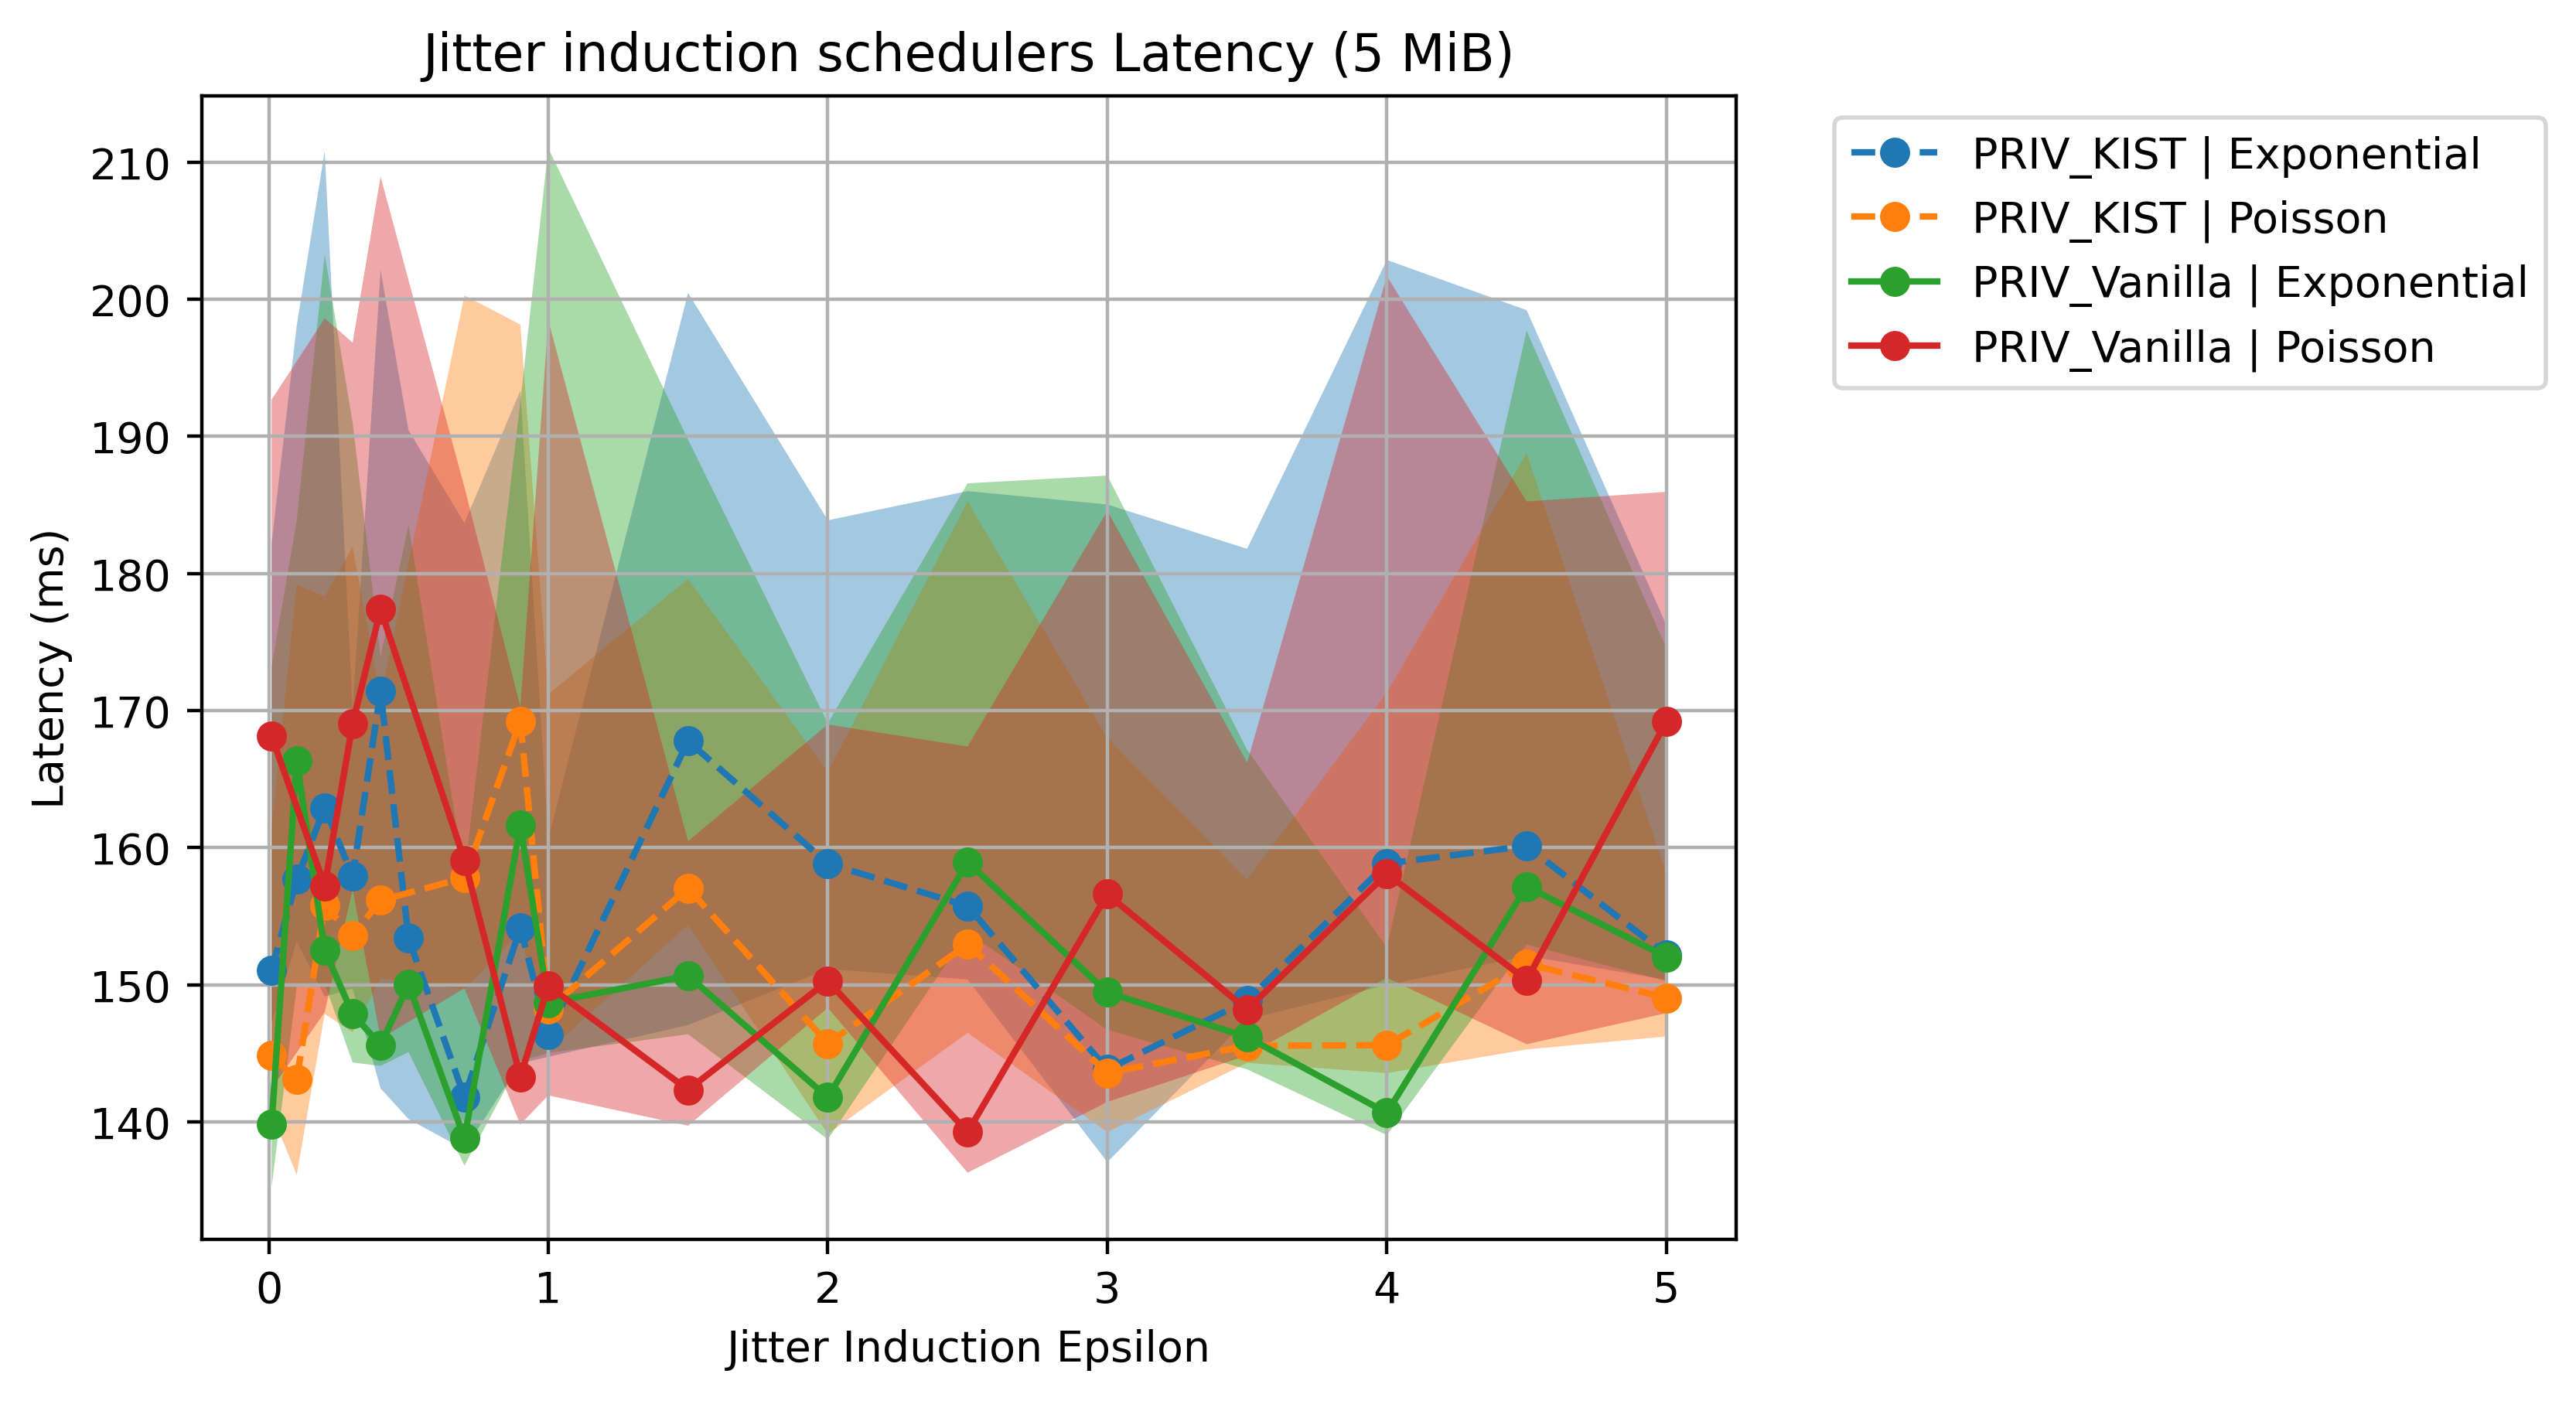
\includegraphics[width=\linewidth]{Chapters/Figures/Plots/dist_latency_50_jitter_5mib.png}}
    \end{subcaptionbox}
    \vfill
    \begin{subcaptionbox}{Both Features\label{fig:dist_both_latency}}[0.70\textwidth]
        {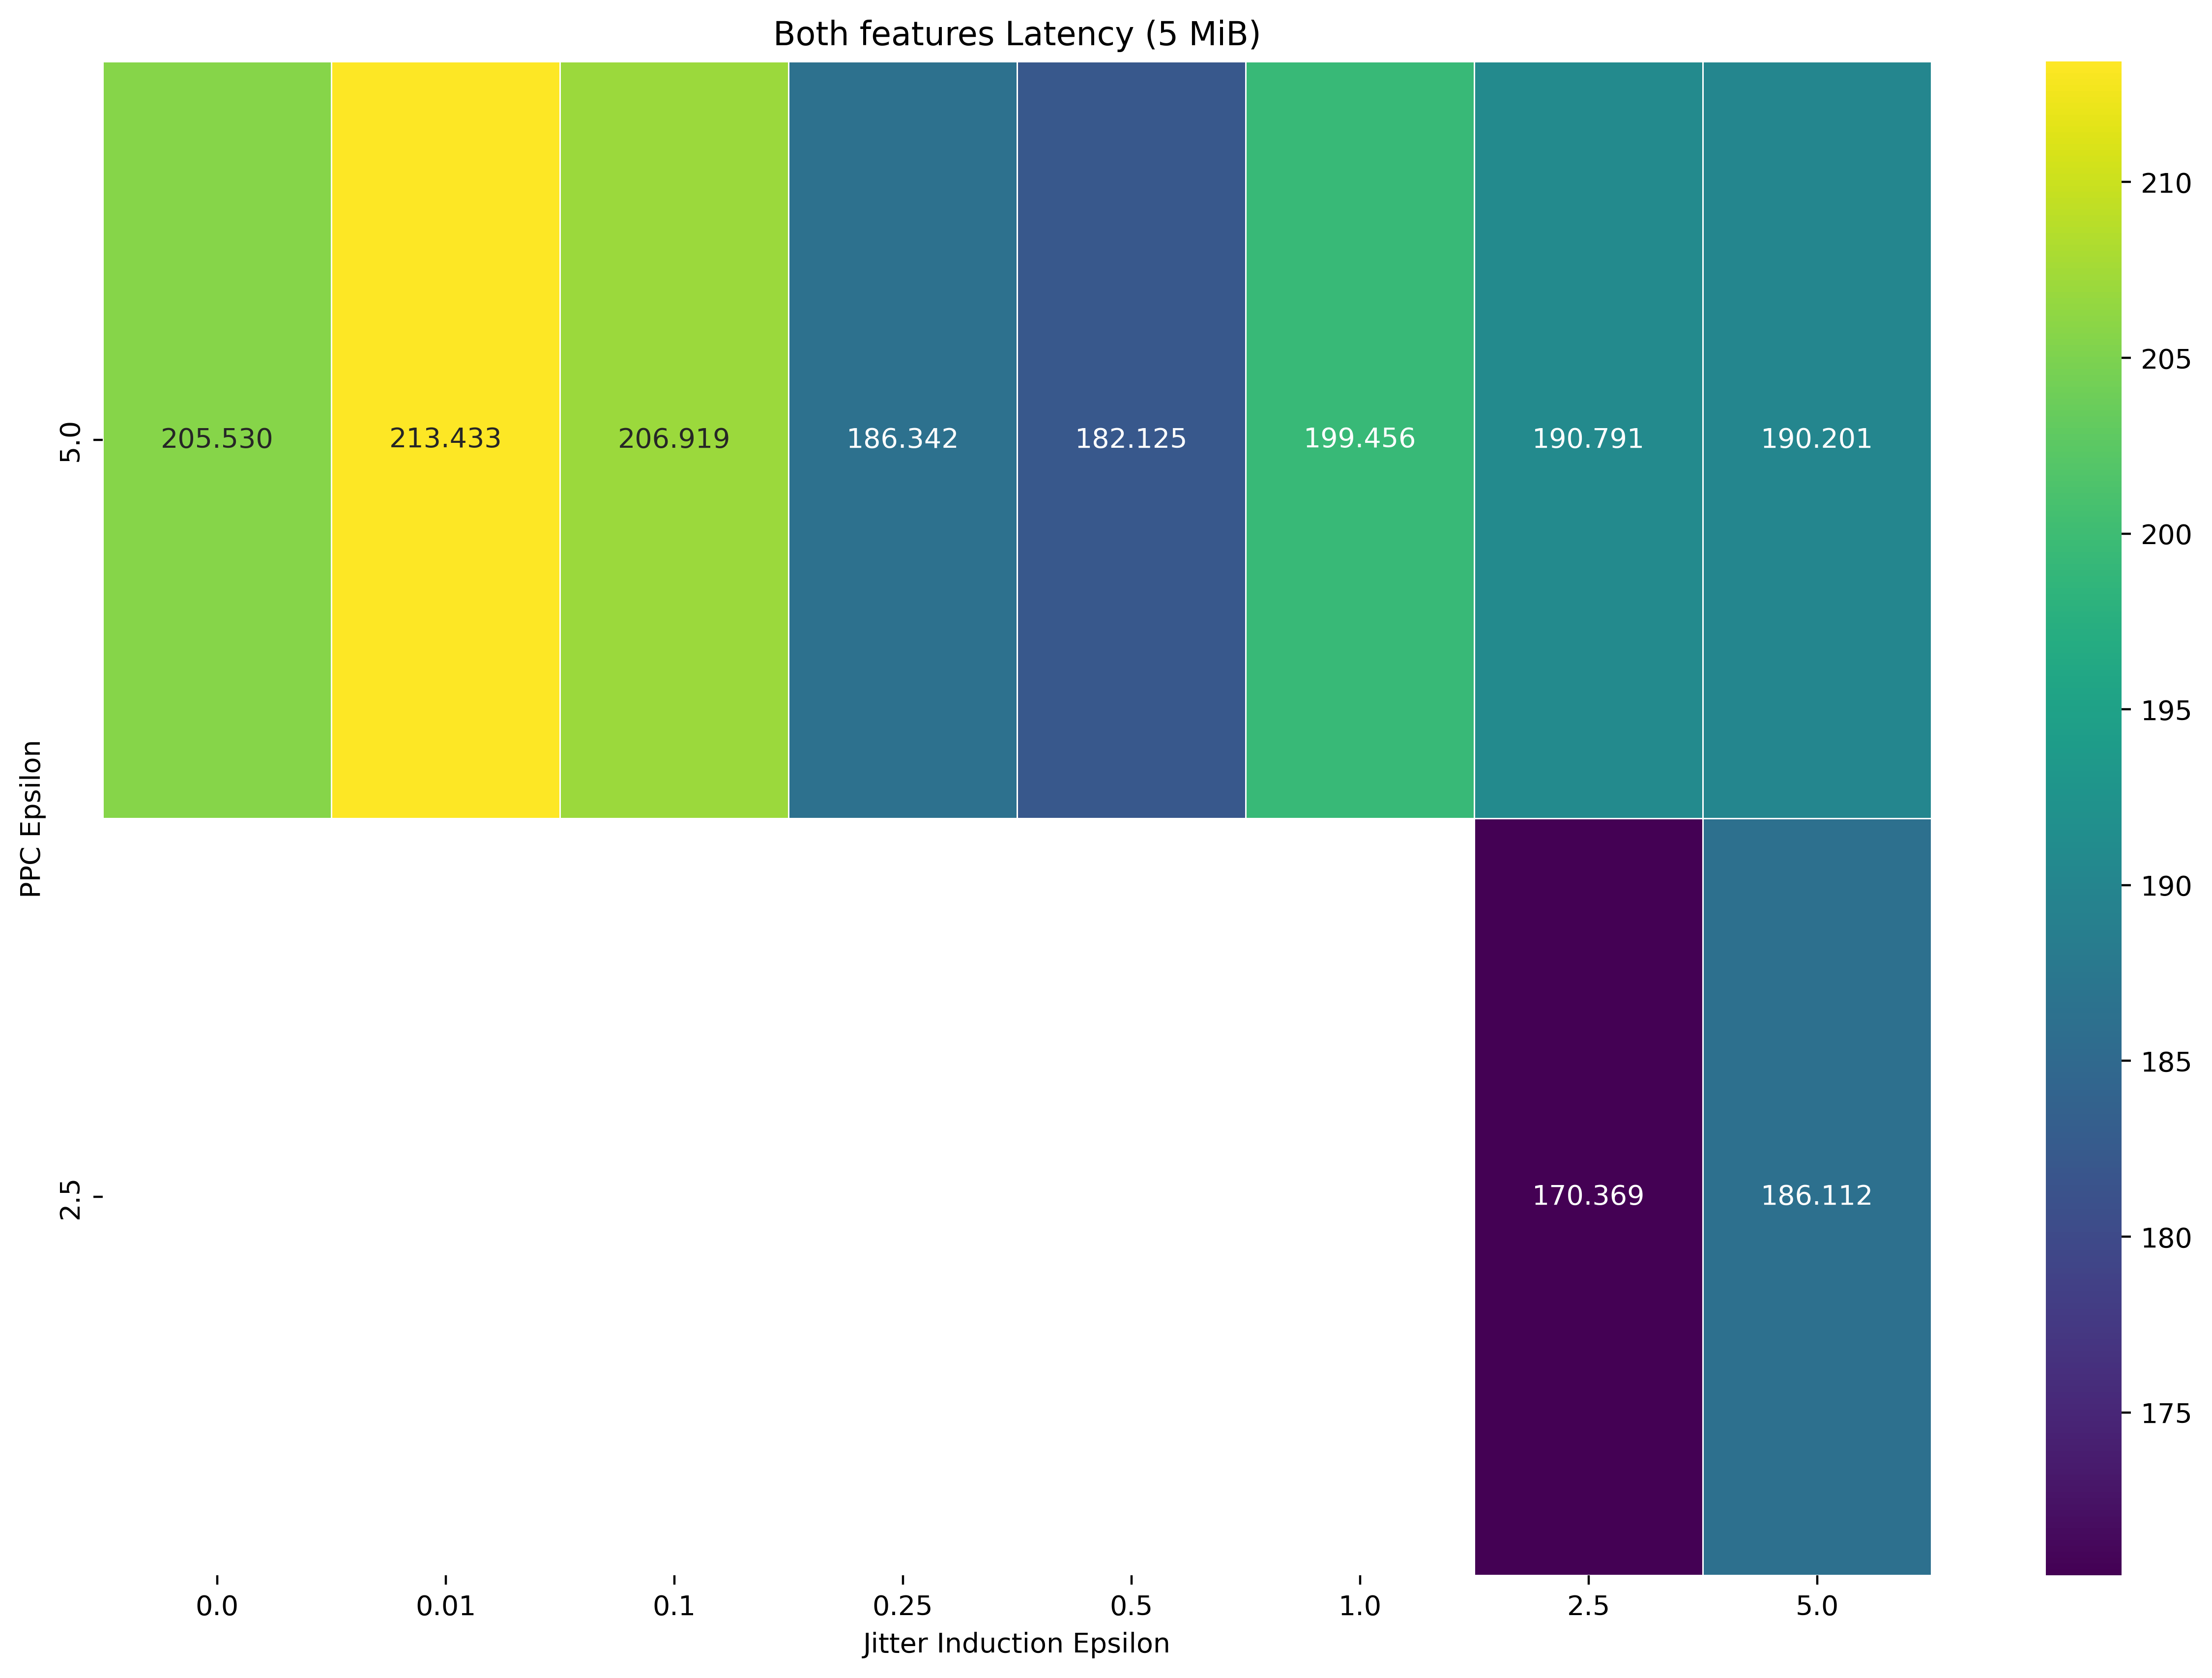
\includegraphics[width=\linewidth]{Chapters/Figures/Plots/dist_latency_50_heatmap_5mib.png}}
    \end{subcaptionbox}
    \caption{Latency Results on Distributed Environment}\label{fig:dist_latency}
\end{figure}

Unlike the previous metrics, the latency results are more sensitive to the schedulers jitter than to the PPC feature. As presented in~\autoref{fig:local_jitter_latency} and~\autoref{fig:dist_jitter_latency}, the Packet Padding Cells feature does not significantly impact the latency results, maintaining a relatively stable latency throughout the experiments. On the other hand, the Schedulers feature shows a more pronounced effect on latency, with noticeable increase when $\epsilon_{J}$ gets closer to 0, and reaching a minimum when $\epsilon_{J}$ is greater than 2. In the distributed environment, the latency results had a higher variance and a less noticeable increase in latency, as described before.
As the time of conduction this evaluation, Tor Metrics reported a median latency of 280 ms. As reported in~\autoref{tab:latency_summary}, the worse latency experience by our evaluation was 213.43 ms, with both features. This table also clearly shows that the impact of both features on latency are less apart as the impact differences produced in throughput and total time evaluations. 
%TODO: MUST TEST COMBINATIONS ON DISTRIBUTED TO GET BETTER ANALYSIS ON WORSE/BETTER TEST BENCH AND CONFIGURATION
\begin{table}[htbp]
    \centering
    \begin{tabular}{|c|c|c|}
    \hline
    \textbf{Configuration} & \textbf{Local} & \textbf{Distributed}\\
    \hline
    Tor Metrics & \multicolumn{2}{c|}{280}  \\ 
    \hline
    \multirow{2}{*}{Control} & 30.59 & 181.36 \\ 
    & 30.53 & 192.54\\
    \hline
    Only PPC & 27.45 – 33.03 & 134.16 – 188.30\\
    \hline
    Only Jitter & 27.45 – 40.66 & 138.81 – 181.95 \\
    \hline
    PPC \& Jitter & 31.40 – 45.44 & 170.37 – 213.43\\
    \hline
    \end{tabular}
    \caption{Latency Results Summary (ms)}\label{tab:latency_summary}
\end{table}

\FloatBarrier
\subsection{TLS Packets and Cells Analysis}

Finally, we present the results of our analysis on the number of false cells, the ratio of false cells, and the total number of TLS packets. These results are not directly comparable to the previous metrics, nor are addressed by Tor Metrics, but we consider relevant to demonstrate and validate the Packet Padding Cells generation and its direct influence in traffic shaping.

\begin{figure}[htbp]
    \centering
    \begin{subcaptionbox}{Number of False Cells\label{fig:local_dummy_count}}[0.45\textwidth]
        {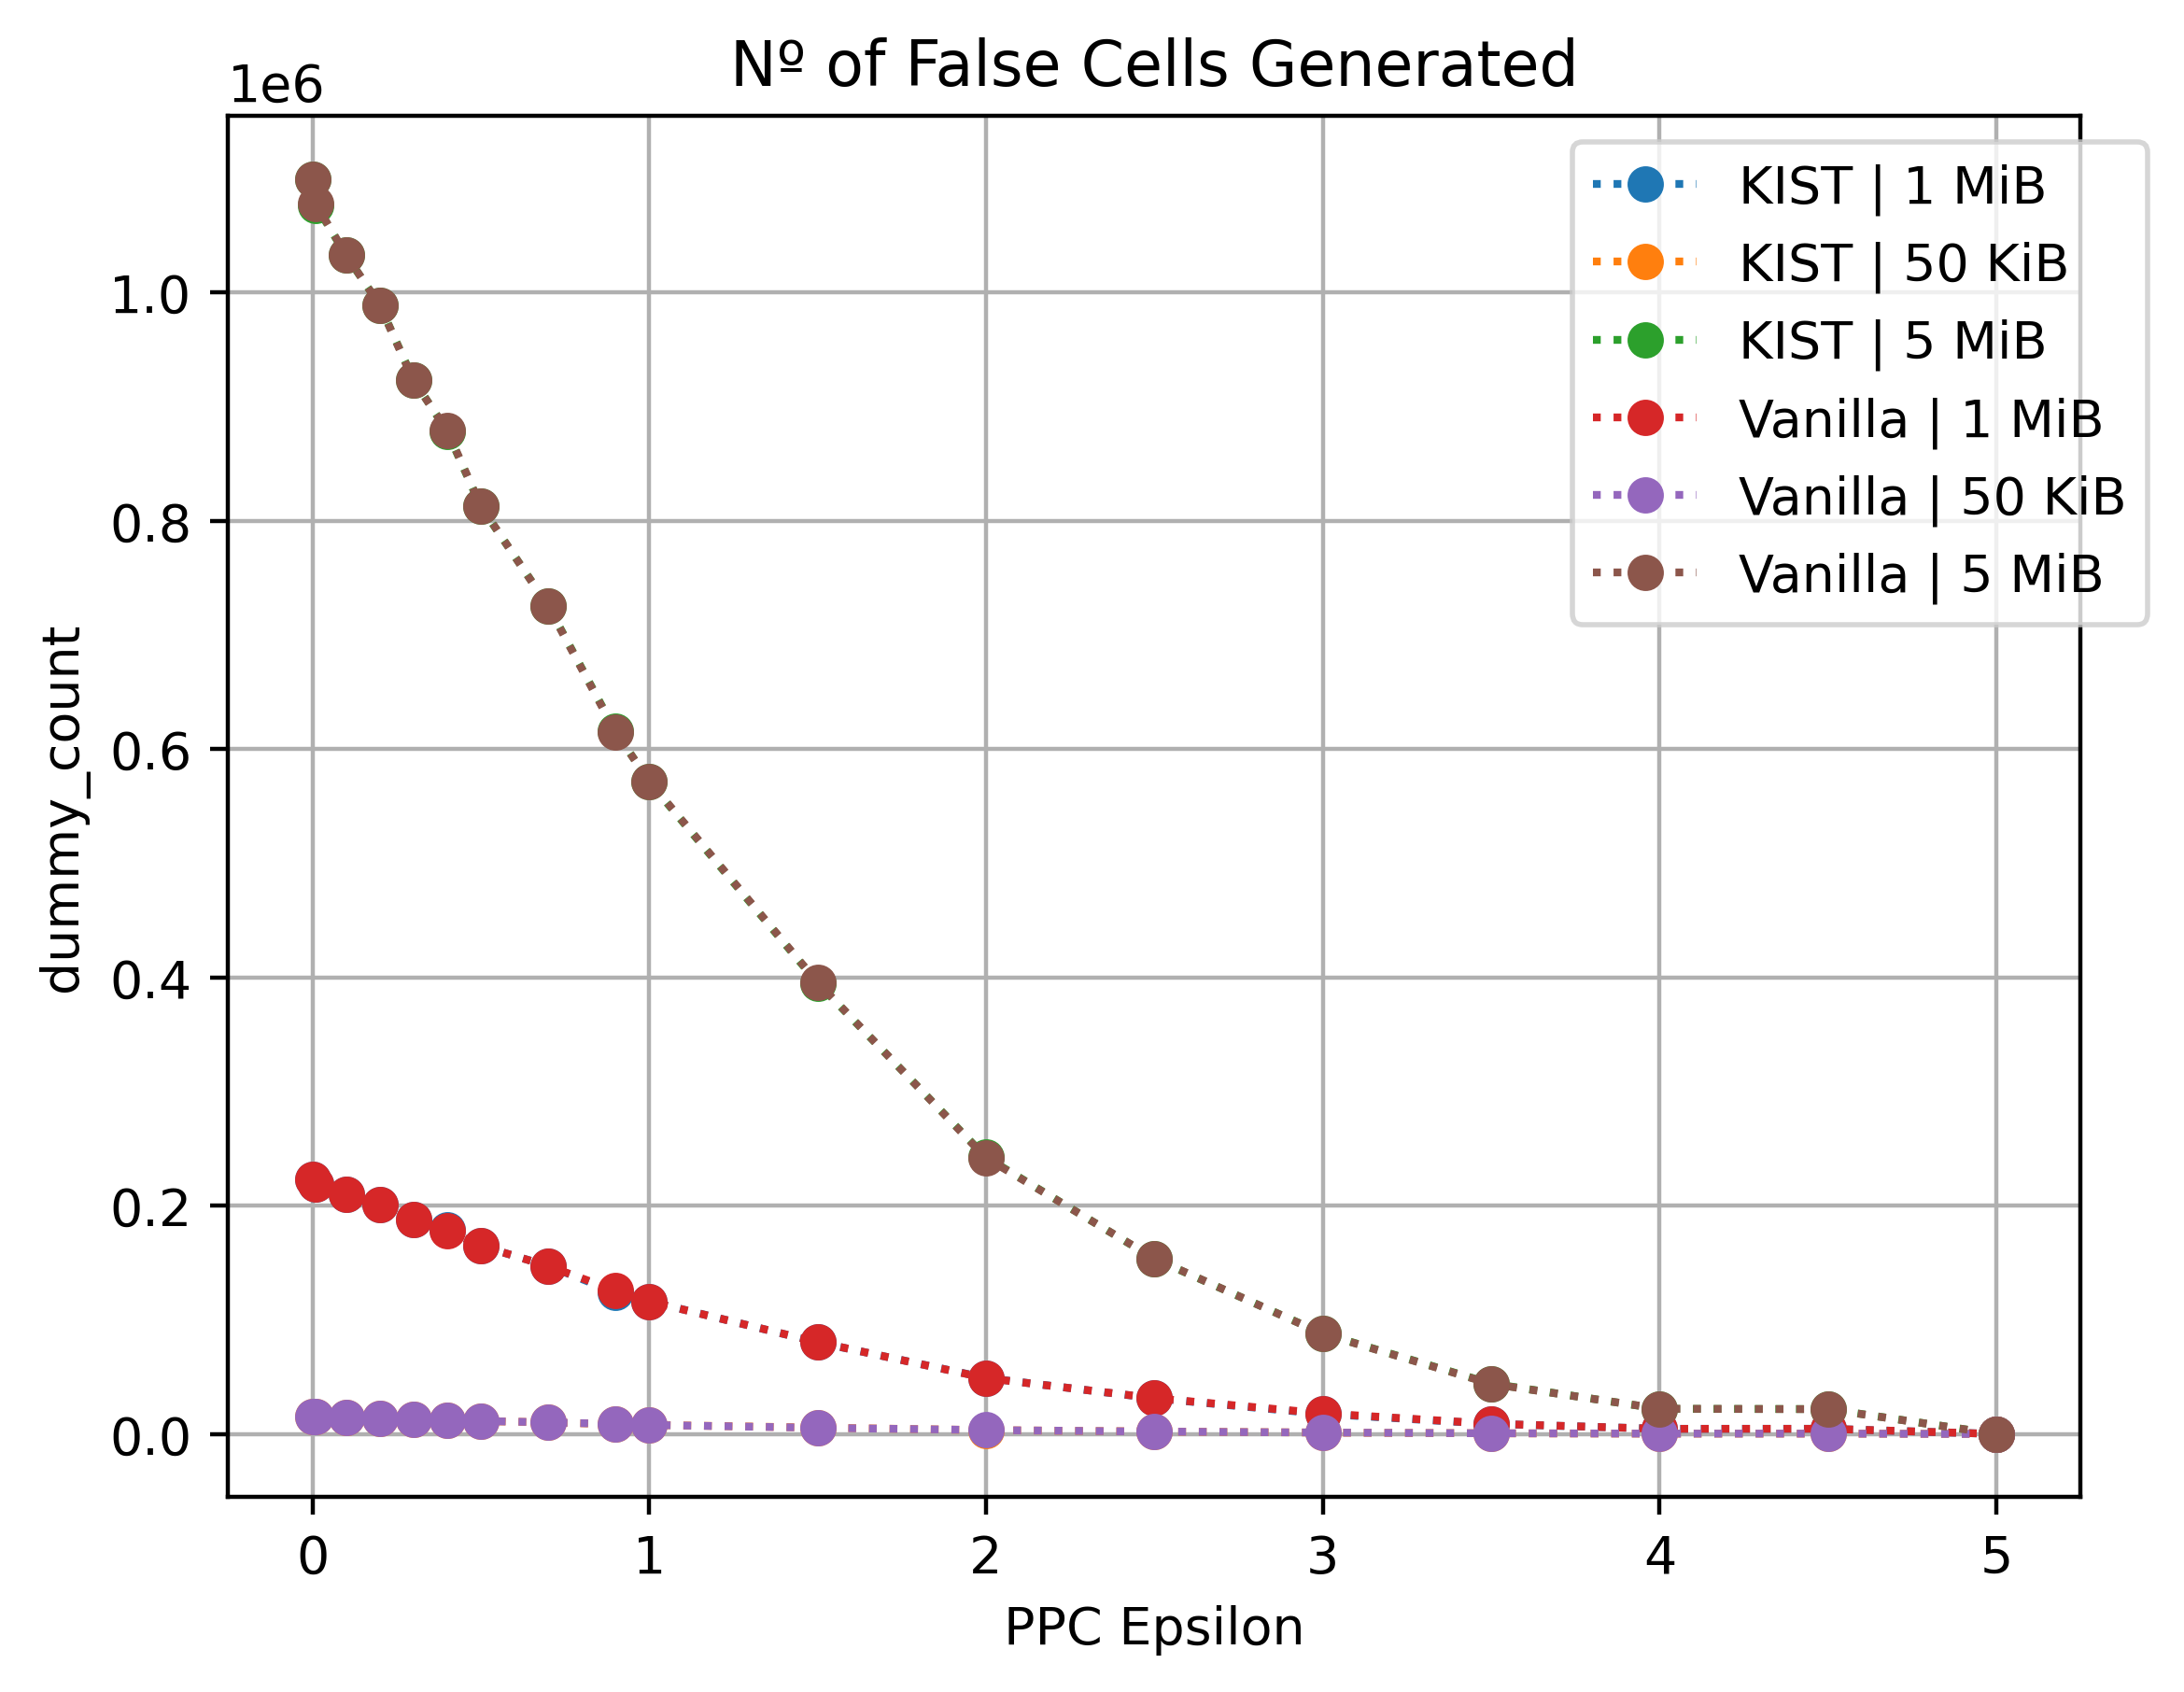
\includegraphics[width=\linewidth]{Chapters/Figures/Plots/local_PPC_count.png}}
    \end{subcaptionbox}
    \hfill
    \begin{subcaptionbox}{Ratio of False Cells\label{fig:local_dummy_ratio}}[0.45\textwidth]
        {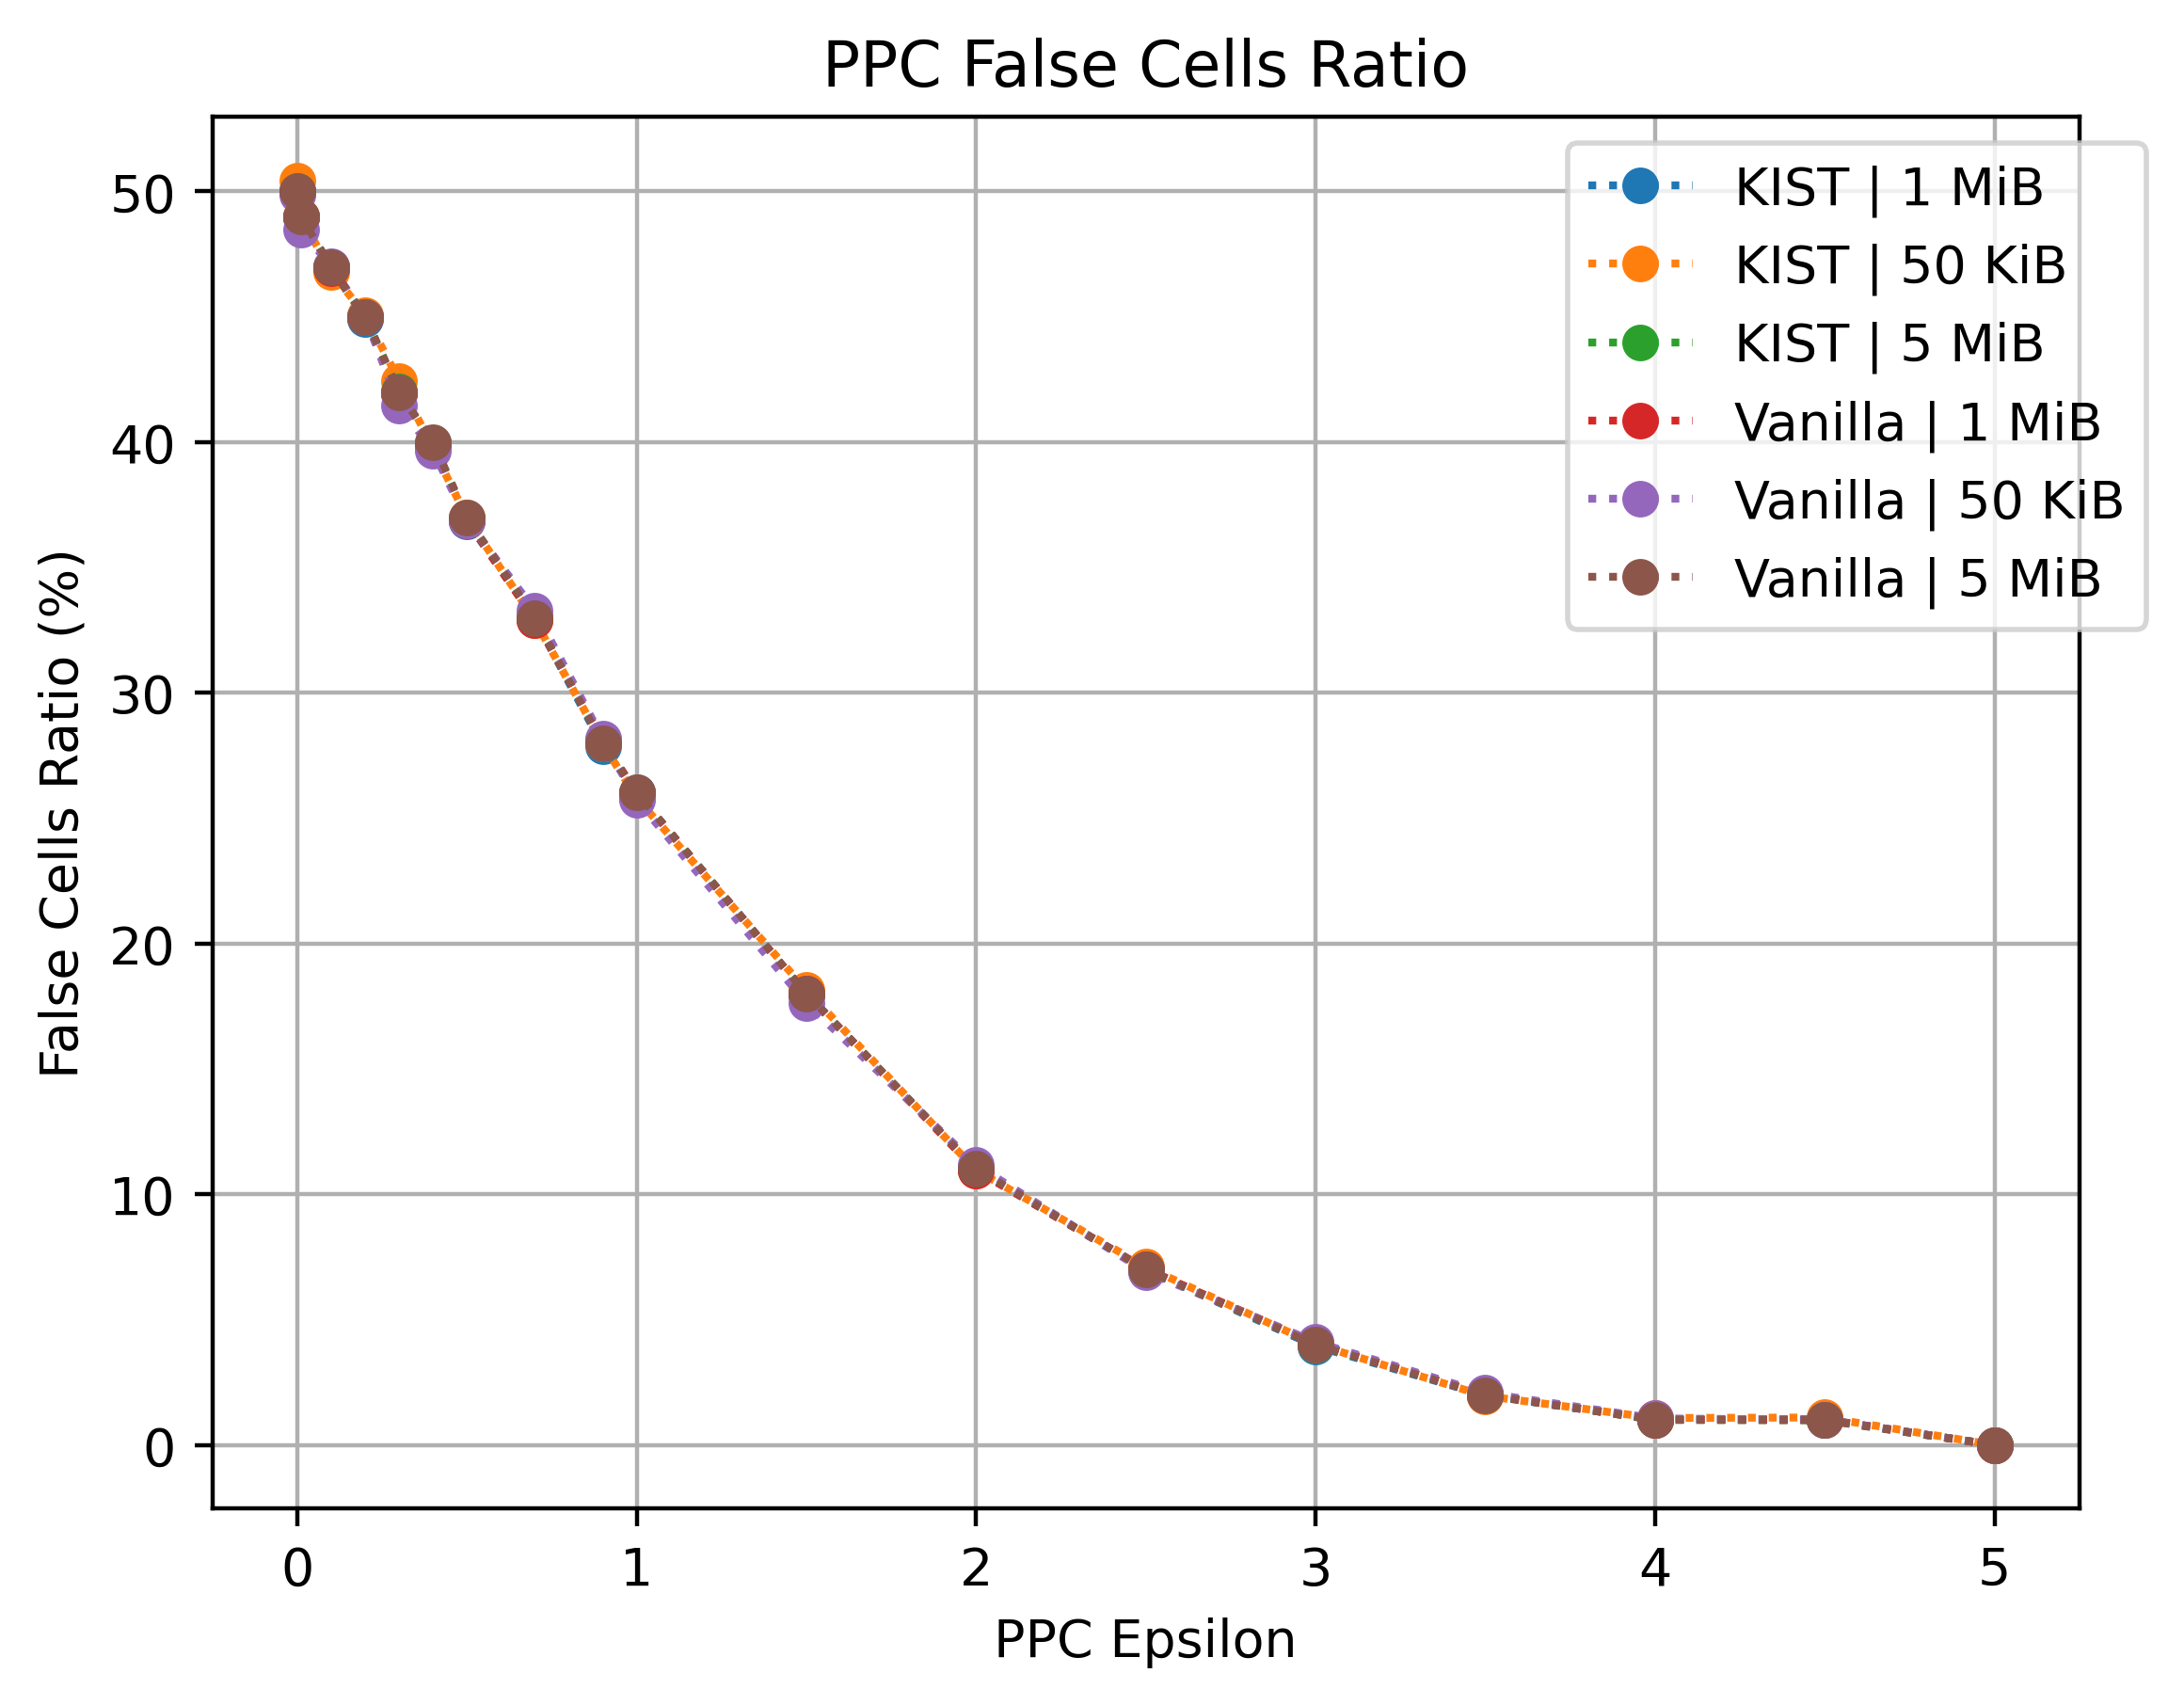
\includegraphics[width=\linewidth]{Chapters/Figures/Plots/local_PPC Ratio_5mib.png}}
    \end{subcaptionbox}
    \vfill
    \begin{subcaptionbox}{Total TLS Packets\label{fig:local_packet_count}}[0.70\textwidth]
        {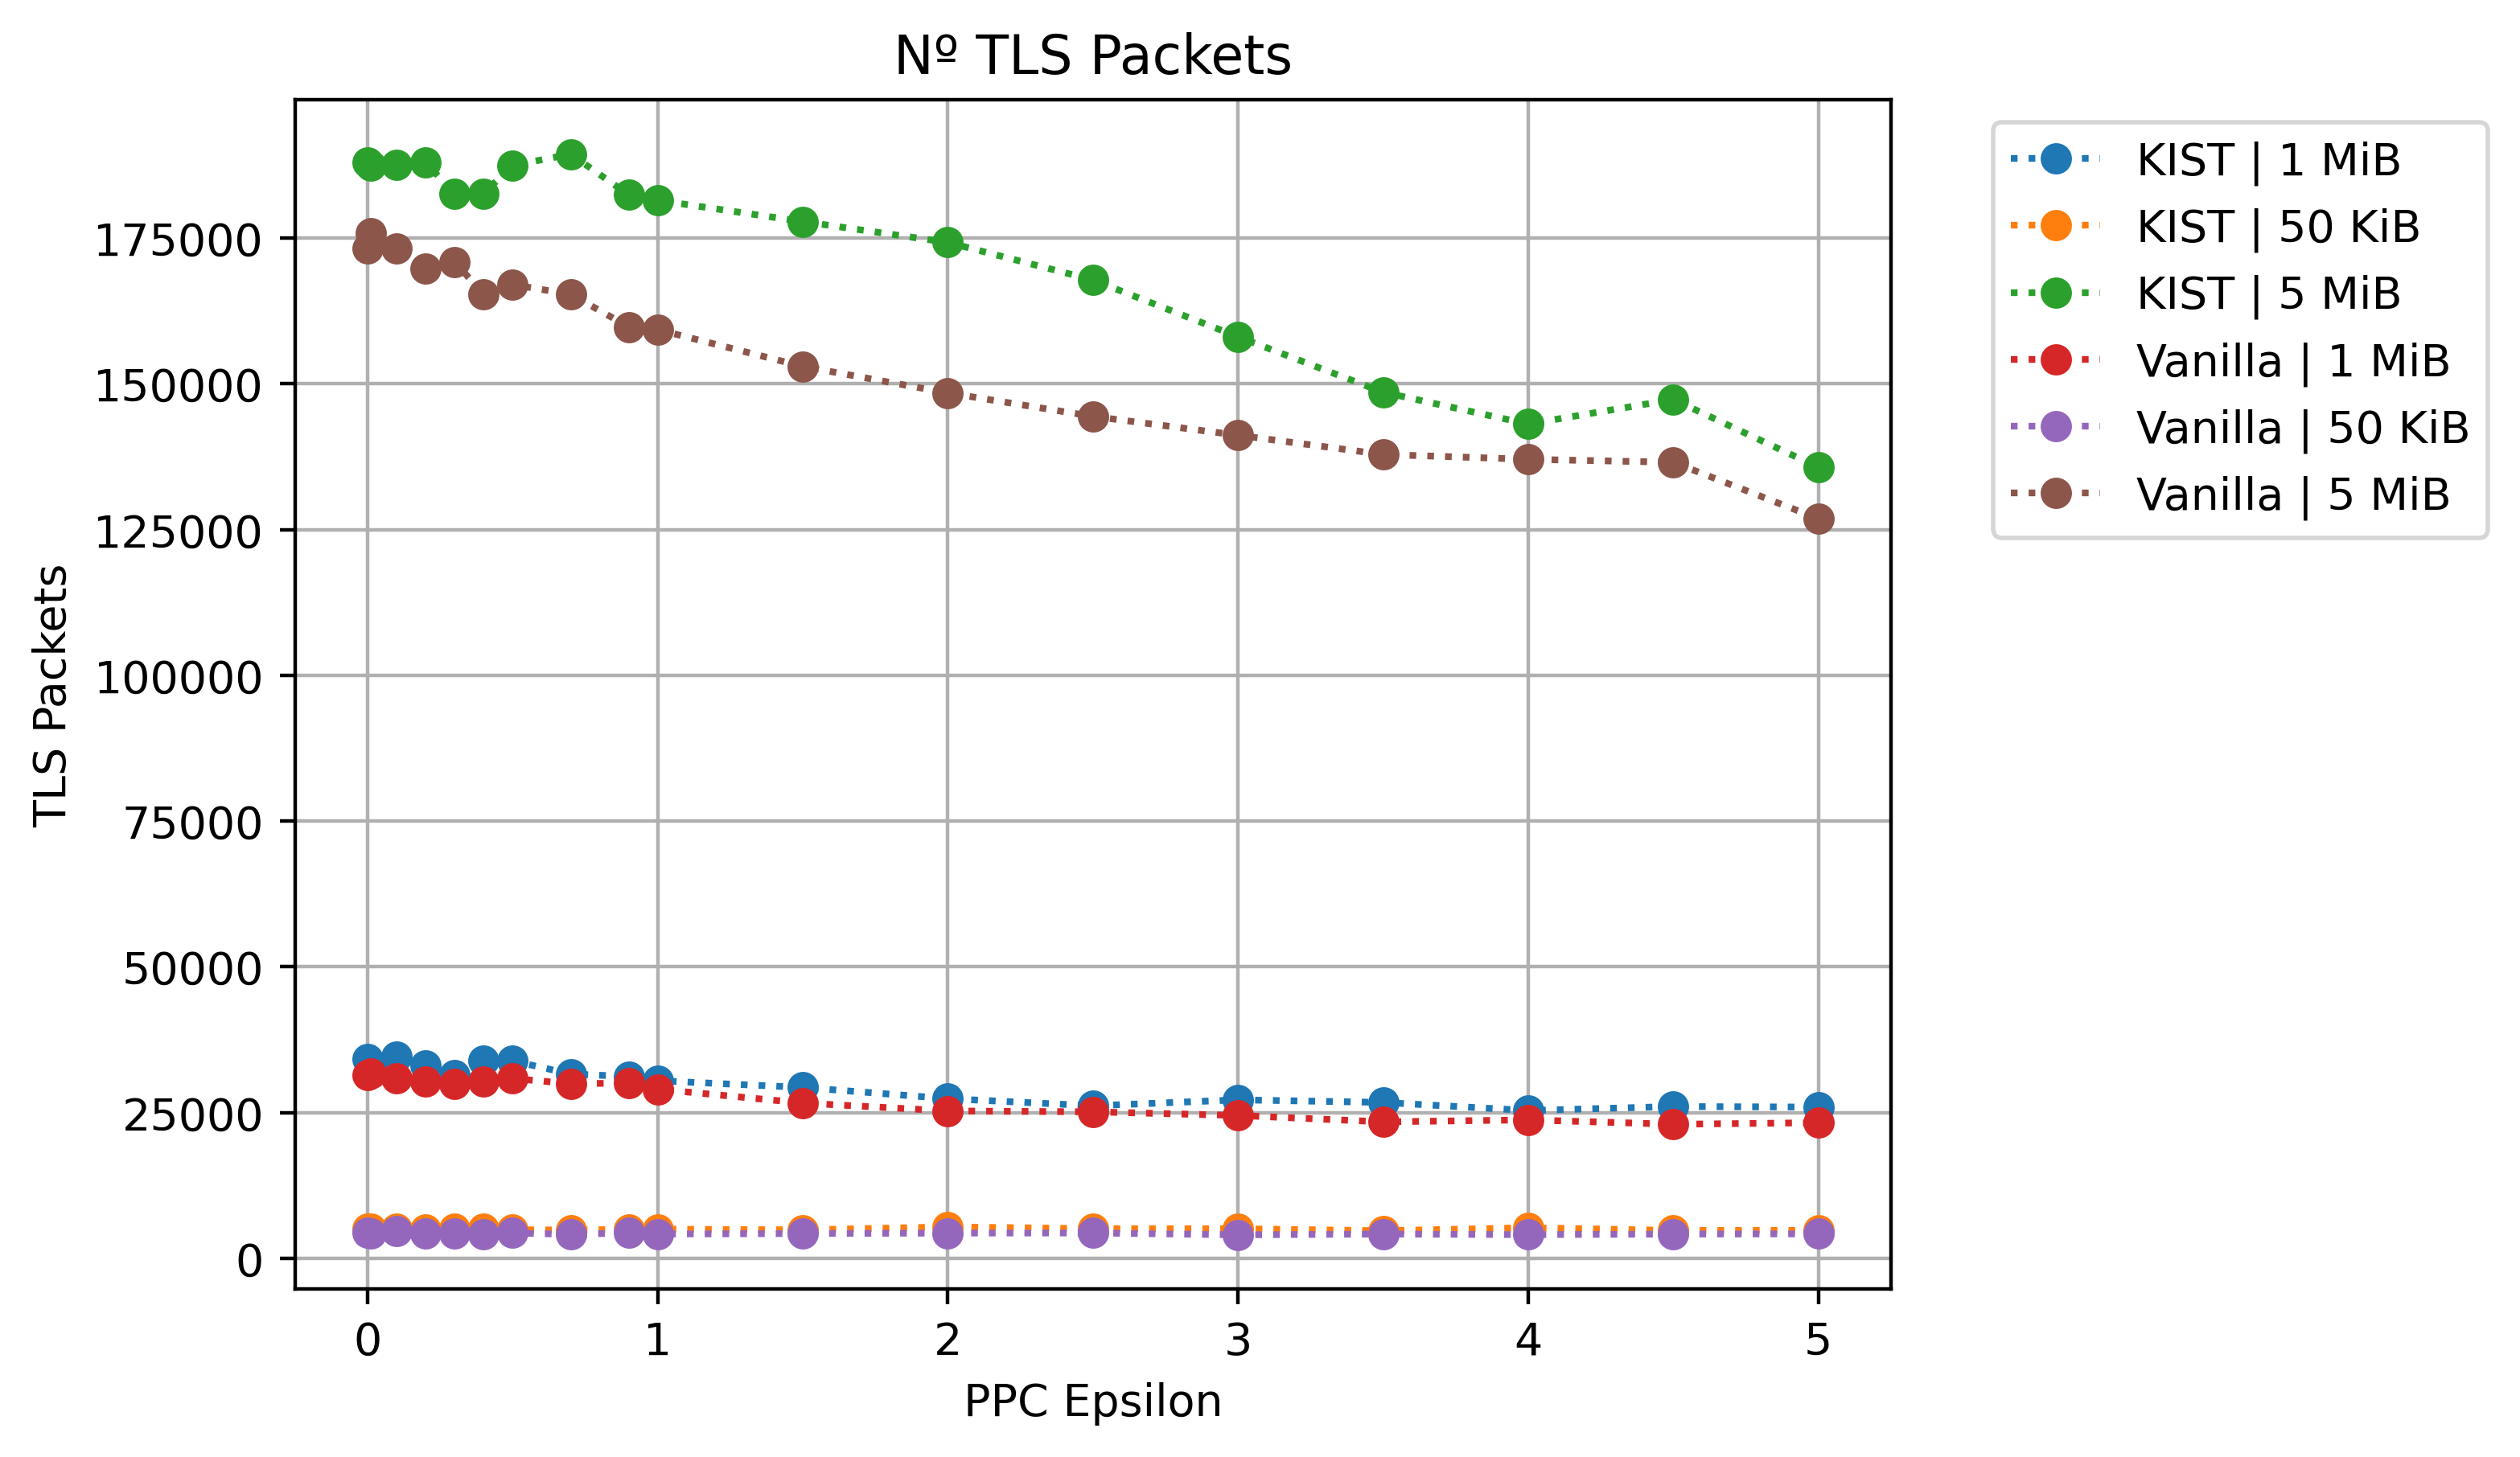
\includegraphics[width=\linewidth]{Chapters/Figures/Plots/local_packet_count_5mib.png}}
    \end{subcaptionbox}
    \caption{Cells and Packets Results}\label{fig:cell_packets_results}
\end{figure}

As expected, the number of false cells and their ratio to total cells decreases as the $\epsilon$ increases, with the highest ratio being $50\%$ when $epsilon_d = 0$. However, we observed that the total number of TLS packets does not follow a directly proportional pattern to the number of false cells, as each TLS packet can contain multiple cells, thereby adding some randomness to the traffic metadata and shape. 

\section{Unobservability Evaluation}\label{sec:unobservability_evaluation}

In this section, we evaluate the resistance of our system, focusing on the capability to withstand website fingerprinting attacks. As mentioned before in~\autoref{subsubsec:website_fingerprinting_attack}, this form of traffic analysis aims to identify the websites a user is visiting, by trying to infer the user traffic and analyzing encrypted traffic patterns.
The following subsections present the methods and tools used to perform our evaluation and the experimental observations.  

\subsection{Methods and Tools}\label{sec:methods_and_tools}

To evaluate the resistance of our system against website fingerprinting attacks, we collected traces of website accesses to be used to train and test several machine learning models. We selected 100 websites from the Tranco Top 1M website list~\cite{LePochat2019}, and sampled each website 50 times, generating 5 000 samples per test configuration. The traces were captured using \texttt{tcpdump} to generate a \textit{pcap} for each sample and for each circuit segment. The website access was simulated by executing \texttt{curl} requests to the list of websites. To perform these requests, we disabled caching to ensure that each request was treated as a new visit. The captured \textit{pcap} files recorded all packet-level network activity, such as packet size, timing, and direction, thus used to evaluate resistance to fingerprinting attacks. 

\subsubsection{Machine Learning Models}

With the before-mentioned traces and to perform the unobservability evaluation, we took inspiration in~\autocite{MIRACE} work on the evaluation of website fingerprinting attacks resistance and employed a diverse set of machine learning models used in traffic analysis research. These models include Naïve Bayes, Logistic Regression, K-Nearest Neighbors (KNN), Support Vector Machines (SVM), Random Forest, Extra Trees, Gradient Boosting, and XGBoost. These models were trained and tested using their default configurations without performing hyperparameter tuning to ensure consistency and provide a fair benchmark. They were trained using 80\% of the collected data, leaving the other 20\% for testing. Below we briefly summarize each of the used models:

\paragraph{Naïve Bayes:} A probabilistic classifier that applies Bayes' theorem and assumes a strong assumption of feature independence (naive). Its interpretability makes it a useful first step in assessing basic traffic features.
\paragraph{Logistic Regression:} A linear classification model that predicts the probability of a binary outcome based on a logistic function. It is frequently used for its simplicity and interpretability in classification tasks, especially when the data is linearly separable.
\paragraph{K-Nearest Neighbors (KNN):} A non-parametric, instance-based learning algorithm that predicts by finding the most common class among the k-nearest neighbors of a data point. It is particularly valuable when the structure of the data is unknown or highly non-linear
\paragraph{Support Vector Machines (SVM):} A robust classification algorithm that finds the optimal hyperplane to best separate data points of different classes in high-dimensional space. It excels in scenarios where data is not linearly separable by transforming input features via kernel functions.
\paragraph{Random Forest:} An ensemble learning method that builds multiple decision trees during training and outputs the class that represents the majority vote from individual trees. Random Forest reduces overfitting and improves generalization by introducing randomness in both feature selection and sample selection, and it is particularly useful for finding intricate features by capturing different patterns and variations across different labels.
\paragraph{Extra Trees:} Similar to Random Forest, but it introduces further randomness by selecting random thresholds for splitting trees, which helps reduce variance and improve predictive performance, especially in noisy datasets.
\paragraph{Gradient Boosting:} An ensemble learning method that sequentially builds models, with each new model correcting errors made by the previous ones. It is highly effective in capturing complex patterns through iterative improvements. This model helps detect nuanced traffic characteristics that may evade simpler classifiers, such as subtle variations in packet size or timings.
\paragraph{XGBoost:} An optimized version of Gradient Boosting, known for its computational efficiency and superior performance. It incorporates regularization techniques that prevent overfitting and improve model generalization, making it particularly suitable for large datasets. Its ability to model complex, non-linear patterns efficiently enables it to uncover subtle patterns.

\subsubsection{Evaluation Metrics}
To evaluate the capability of our system in mitigating website fingerprinting attacks, we measured each model effectiveness using the following metrics: 

\subsection{Experimental Observations}\label{sec:experimental_observations_unobservability}

\section{Formal Validation}\label{sec:formal_validation}

\section{Discussion}\label{sec:validation_discussion}

\section{Summary}\label{sec:validation_summary}
